\chapter{Testy wydajności}
\label{cha:benchmarks}

Do testów wydajności wykorzystano przykłady napisane przez Joaquín Mª López Muñoz, omówione na konferencji using std::cpp 2015 \cite{MindTheCache}, z pewnymi modyfikacjami.

Główna modyfikacja została przedstawiona na~listingu \ref{lst:measureCode}. Polega ona na~zmianie funkcji mierzącej czas, tak, aby mierzyła ona tylko czas danej operacji -- wywołania funkcji szablonowej \texttt{f()}, przekazywanej przez argument szablonowy lambda. Test wydajności polega na wykonaniu 50 iteracji, w~których mierzony jest czas wykonania przekazanej funkcji. Wyniki kolejnych pomiarów są~wypisywane na~standardowe wyjście, a~następnie uśredniane przez skrypt uruchamiający testy.

Pozostałe modyfikacje polegały głównie na zmianie interfejsu programu, tak, aby dało się uruchomić test wydajności dla odpowiedniego przypadku oraz rozmiaru danych (zamiast liczyć wszystko jednocześnie), dzięki czemu można dokonać analizy narzędziami takimi jak perf, cahegrind czy Intel VTune Amplifier.

\begin{lstlisting}[
caption={Kod funkcji mierzącej czas. Na podstawie \cite{MindTheCache}.},
label=lst:measureCode,
numbers=left,
stepnumber=1,    
firstnumber=1,
numberfirstline=true]
template <int iterations=50, typename Size, typename F>
void measure(Size n, F f) {
    using namespace std::chrono;
    volatile decltype(f()) res{0}; /* to avoid optimizing f() away */
    high_resolution_clock::time_point t1, t2;
    
    std::array<long double, iterations> timings;
    
    for(auto i=0; i<iterations; ++i) {
        t1 = high_resolution_clock::now();
        res += f();
        t2 = high_resolution_clock::now();
        timings[i] = (long double)(t2 - t1).count() / (long double)n;
    }
    std::cerr << "result value used against compiler optimization - ignore this: " << res << std::endl;
    
    for(int i=0; i<iterations-1; ++i)
        std::cout << timings[i] << ",";
    std::cout << timings[iterations-1] << std::endl;
}
\end{lstlisting}

Przedstawione testy zostały przeprowadzone na dwóch różnych maszynach o parametrach przedstawionych w~tabeli \ref{tab:machines}.


\begin{table}[!h]
    \caption{Parametry maszyn na których zostały przeprowadzone testy wydajności.}
    \label{tab:machines}
    \centering
    \begin{tabular}{|5||c|c|}
        \hline
        \textbf{Parametr} & \textbf{Maszyna 1} & \textbf{Maszyna 2}
        \\ \hline \hline
        Model procesora & Intel\textsuperscript{\textregistered} Core\textsuperscript{TM} i7-4720HQ & Intel\textsuperscript{\textregistered} Xeon\textsuperscript{\textregistered} W3565
        \\ \hline
        Taktowanie & 2.60 GHz & 3.20 GHz
        \\ \hline
        Taktowanie turbo & 3.6 GHz & 3.46 GHz
        \\ \hline
        Turbo włączone & nie & nie
        \\ \hline
        Liczba rdzeni & 4 & 4
        \\ \hline
        Hyper-Threading & tak & tak
        \\ \hline
        Liczba wątków & 8 & 8
        \\ \hline
        Pamięć podręczna L1 danych (dla każdego rdzenia) & 32 kB & 32 kB
        \\ \hline
        Pamięć podręczna L1 instrukcji (dla każdego rdzenia) & 32 kB & 32 kB
        \\ \hline
        Pamięć podręczna L2 (dla każdego rdzenia) & 256 kB & 256 kB
        \\ \hline
        Pamięć podręczna L3 (współdzielona między rdzeniami) & 6 MB & 8 MB
        \\ \hline \hline
        System operacyjny & Ubuntu 15.10 & Debian 7.8 (wheezy)
        \\ \hline
        Wielkość strony pamięci & 4 kB & 4 kB
        \\ \hline
        Wersja kompilatora gcc & 5.2.1 (Ubuntu 5.2.1-22ubuntu2)  & 4.7.2 (Debian 4.7.2-5)
        \\ \hline
    \end{tabular}
\end{table}


\section{Przejście po macierzy}
\label{sub:matrixTraversal}

W poniższym przykładzie przeanalizowany został problem zsumowania elementów macierzy~\cite{MindTheCache_MatrixSum}. Porównane zostały dwa sposoby przejścia macierzy, przedstawione w tabeli \ref{tab:matrixTraversal}.

\begin{table}[!h]
	\centering

\caption{Testowany kod operacji sumowania elementów. Komórka na rysunku przedstawia element macierzy w pamięci RAM, która jest reprezentowana od lewej do prawej.}
\label{tab:matrixTraversal}
\begin{tabular}{c 0 c}
\hline 
Przejście macierzy wierszami & & Przejście macierzy kolumnami
\\ \hline \hline
\begin{lstlisting}
long int sum = 0;
for(auto i=0; i<dim; ++i)
    for(auto j=0; j<dim; ++j)
        sum += matrix[i][j];
return sum;
\end{lstlisting} & &
\begin{lstlisting}
long int sum = 0;
for(auto j=0; j<dim; ++j)
    for(auto i=0; i<dim; ++i)
        sum += matrix[i][j];
return sum;
\end{lstlisting}
\\
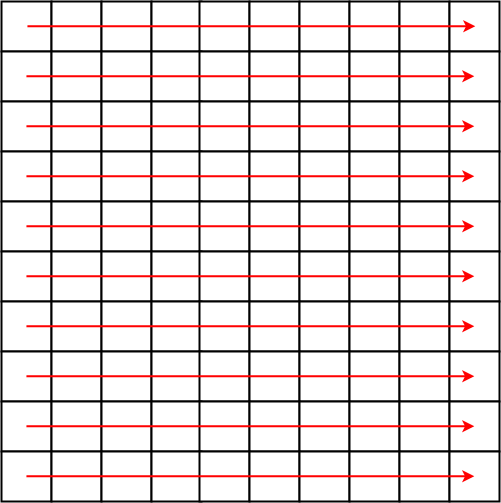
\includegraphics[width=0.25\textwidth]{images/matrix_row}
&  &
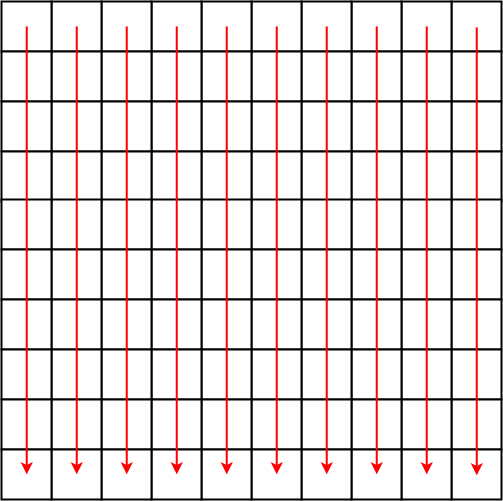
\includegraphics[width=0.25\textwidth]{images/matrix_col}
\\ \hline
\end{tabular}
\end{table}


Wyniki testu wydajności przedstawiono na rysunku \ref{fig:matrixResults}. Najlepszy wynik uzyskano wykorzystując najbardziej agresywną optymalizację -- \texttt{-O3}.
W każdym przypadku przejście wierszami było wydajniejsze od przejścia kolumnami. Przyczyna jest bardzo prosta -- z~uwagi na~to, że~elementy macierzy są~ułożone w~ciągłym obszarze pamięci wierszami, to~dzięki wczesnemu pobieraniu oraz pamięci podręcznej, kolejne wiersze są~pobierane do~cache, podczas gdy procesor sumuje elementy danego wiersza (a w zasadzie danej linii cache).

Gdy~rozmiar macierzy jest dostatecznie mały -- do~$2^{16}$ elementów (czyli 256 kB --~rozmiaru pamięci podręcznej L2), wydajność przetwarzania wierszami jest o około 30-40\% większa od przetwarzania kolumnami.

Po przekroczeniu tego rozmiaru, program stara się wykorzystać pamięć podręczną L3. Ze~względu na~fakt, że~pamięć ta~nie~jest dostępna na~wyłączność programu (ponieważ jest współdzielona między rdzeniami), to~począwszy od~$2^{16}$ elementów wykres dla~przypadku przetwarzania kolumnami jest poszarpany. Po przekroczeniu rozmiaru $2^{21}$ elementów, wykres ten staje się jeszcze bardziej nieregularny. Przyczyną tego mogą być omówione w~rozdziale \ref{cha:Associativity} konflikty oraz zaśmiecanie pamięci podręcznej -- może to być spowodowane konkurowaniem o~miejsce w~pamięci podręcznej L3 z~innymi procesami, bądź po prostu niefortunne ułożenie adresów kolejnych kolumn macierzy (np. mapujących się do tych samych indeksów w cache).

W~tabeli \ref{tab:matrixSumPerf} przedstawiono wyniki programu perf dla~wybranych rozmiarów macierzy. Ciekawymi przypadkami są~punkty $2^{22}$, $2^{24}$ oraz $2^{26}$ --~charakterystyczne piki na~wykresach wydajności. Mają one ponad 90\% chybień do~pamięci podręcznej L3, stąd prawdopodobnie występuje w nich największy efekt konfliktów lub zaśmiecania pamięci podręcznej.

Na rysunku \ref{fig:matrixResultsXeon} zostały przedstawione wykresy pomiarów wykonanych na maszynie z~procesorem Intel Xeon W3565. Wykresy te~są~dużo mniej poszarpane, co może wynikać z~mniejszego obciążenia systemu. Na wykresie \ref{fig:matrixResultsO3Xeon} można także zaobserwować trzy charakterystyczne piki omówione wcześniej. Być może ma to związek z~rozmiarem strony pamięci (4 kB), gdyż odległości między kolejnymi elementami, po których program przechodzi wynoszą 8 kB, 16 kB oraz 32 kB. Przypadki te wymagają dogłębniejszej analizy.

\begin{figure}[!h]
	\centering
	\begin{subfigure}[c]{0.45\textwidth}
		\centering
		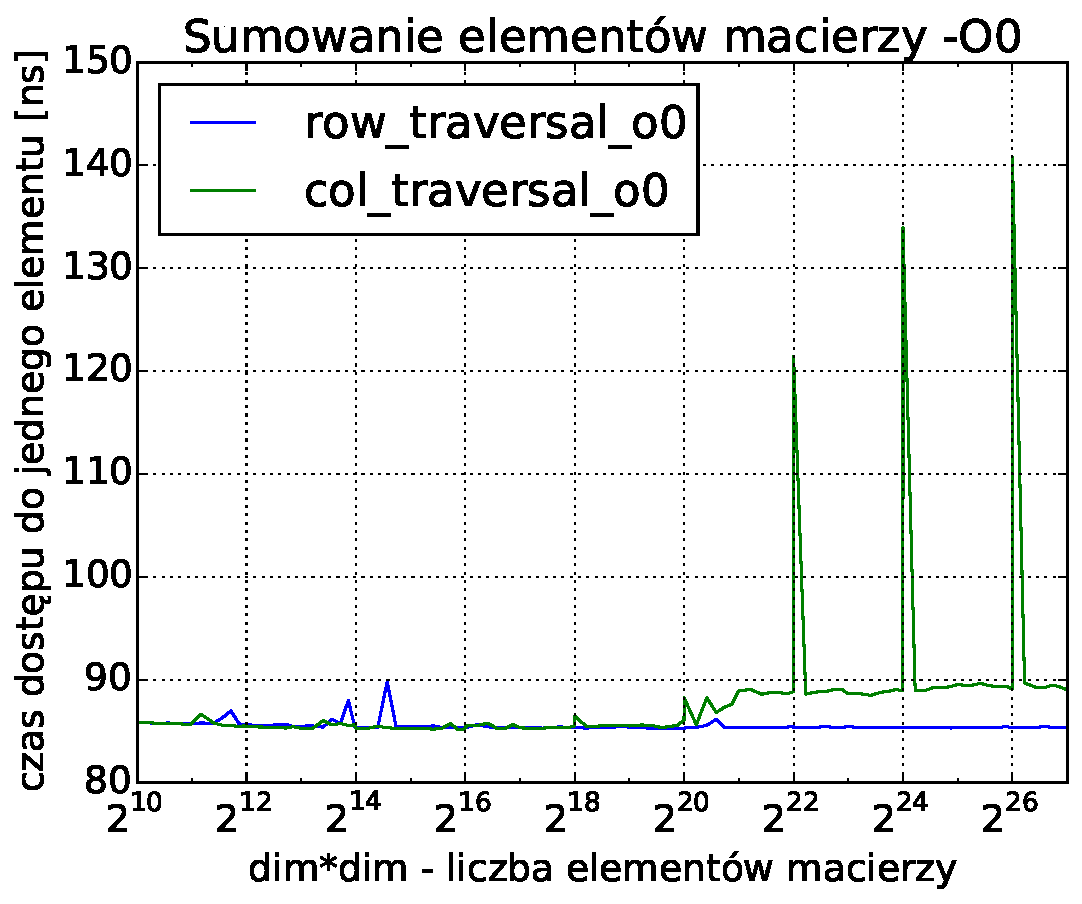
\includegraphics[width=\textwidth]{images/benchs/matrix_sum_O0}
		\caption{Kompilacja z flagą \texttt{-O0}}
	\end{subfigure}
	~
	\begin{subfigure}[c]{0.45\textwidth}
		\centering
		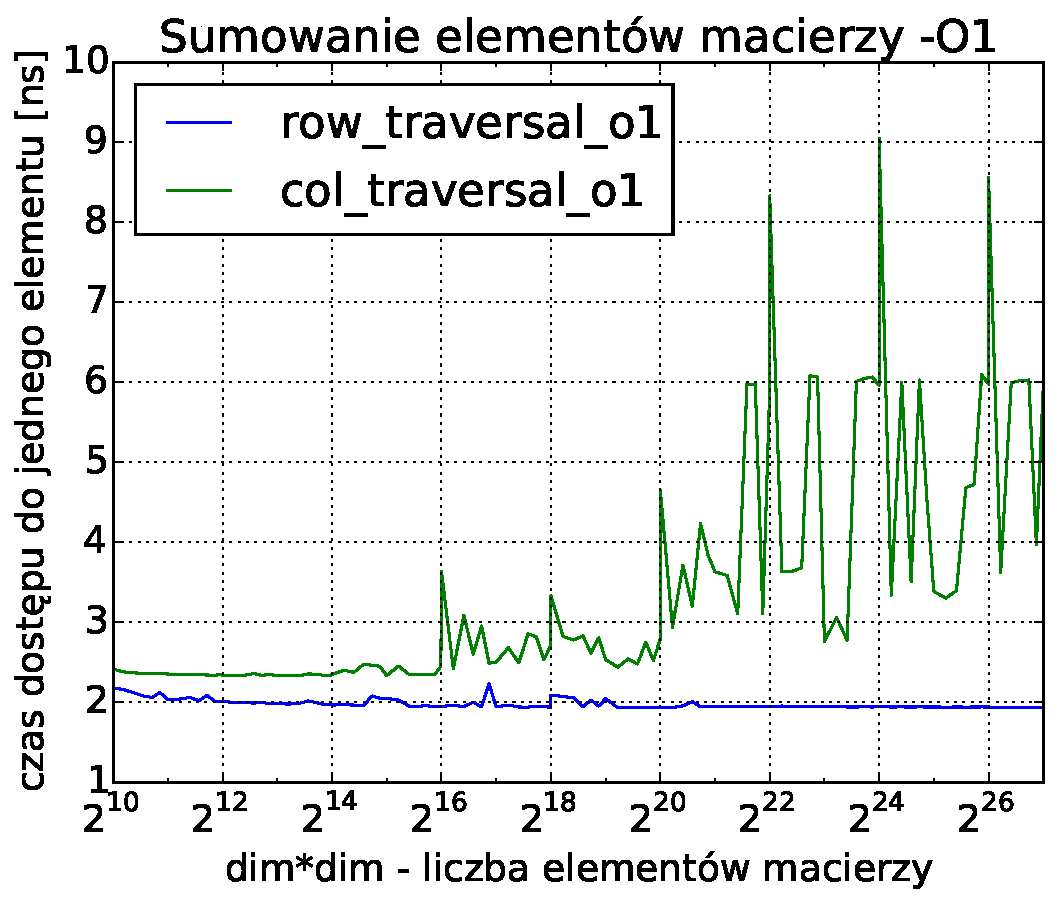
\includegraphics[width=\textwidth]{images/benchs/matrix_sum_O1}
		\caption{Kompilacja z flagą \texttt{-O1}}
	\end{subfigure}
	\\
    \vspace{0.4cm}
	\begin{subfigure}[c]{0.45\textwidth}
		\centering
		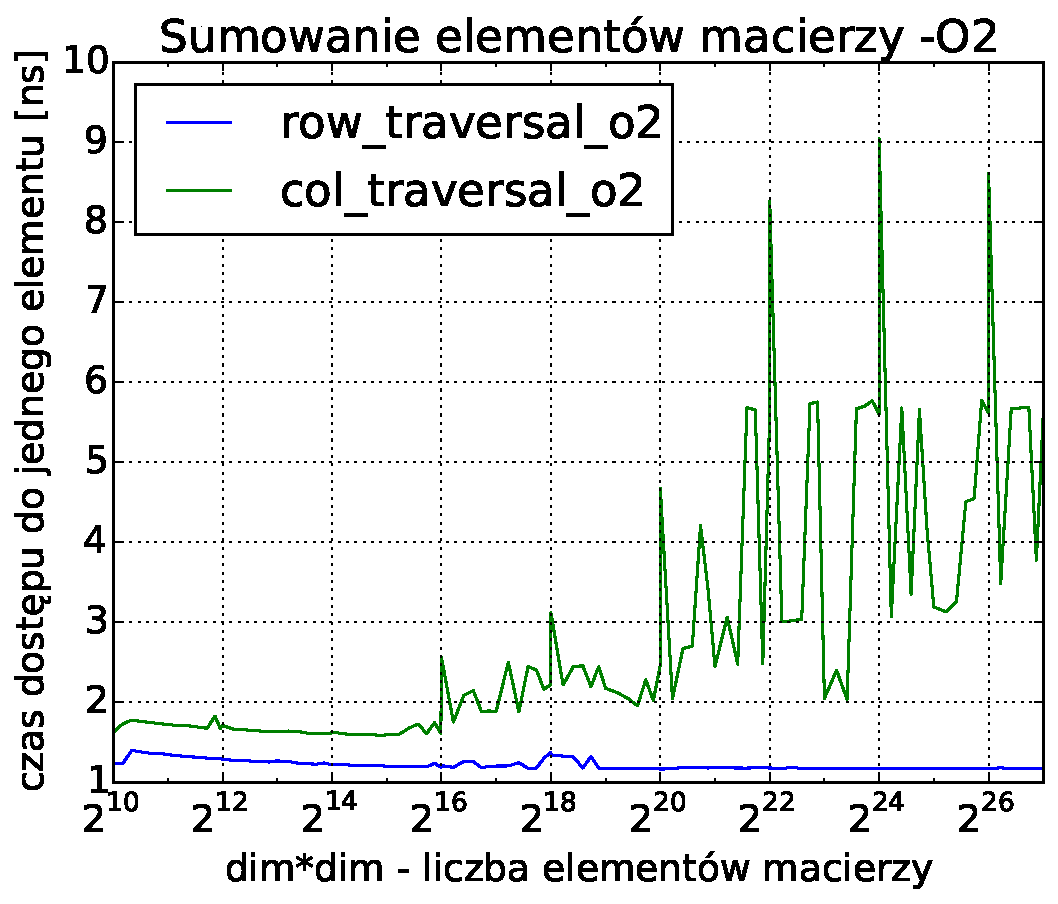
\includegraphics[width=\textwidth]{images/benchs/matrix_sum_O2}
		\caption{Kompilacja z flagą \texttt{-O2}}
	\end{subfigure}
	~
	\begin{subfigure}[c]{0.45\textwidth}
		\centering
		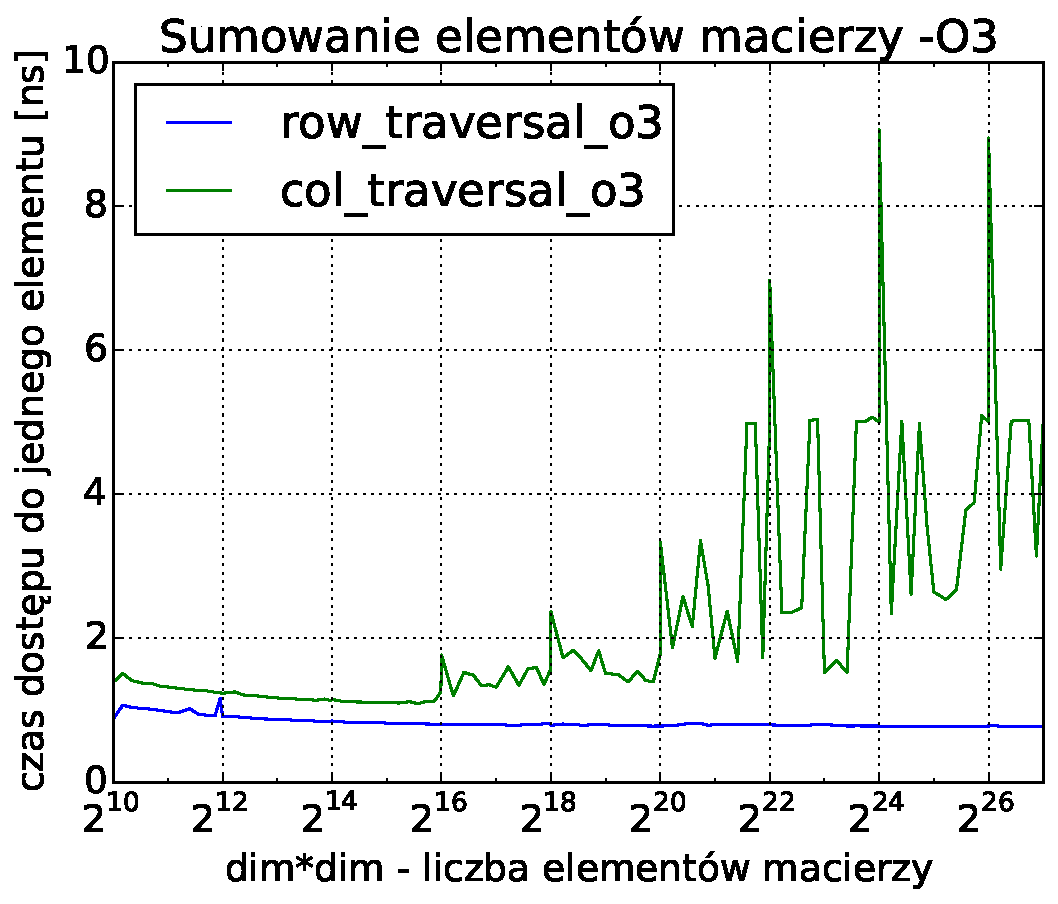
\includegraphics[width=\textwidth]{images/benchs/matrix_sum_O3}
		\caption{Kompilacja z flagą \texttt{-O3}}
	\end{subfigure}
    \\
    \vspace{0.4cm}
    \begin{subfigure}[c]{1.0\textwidth}
        \centering
        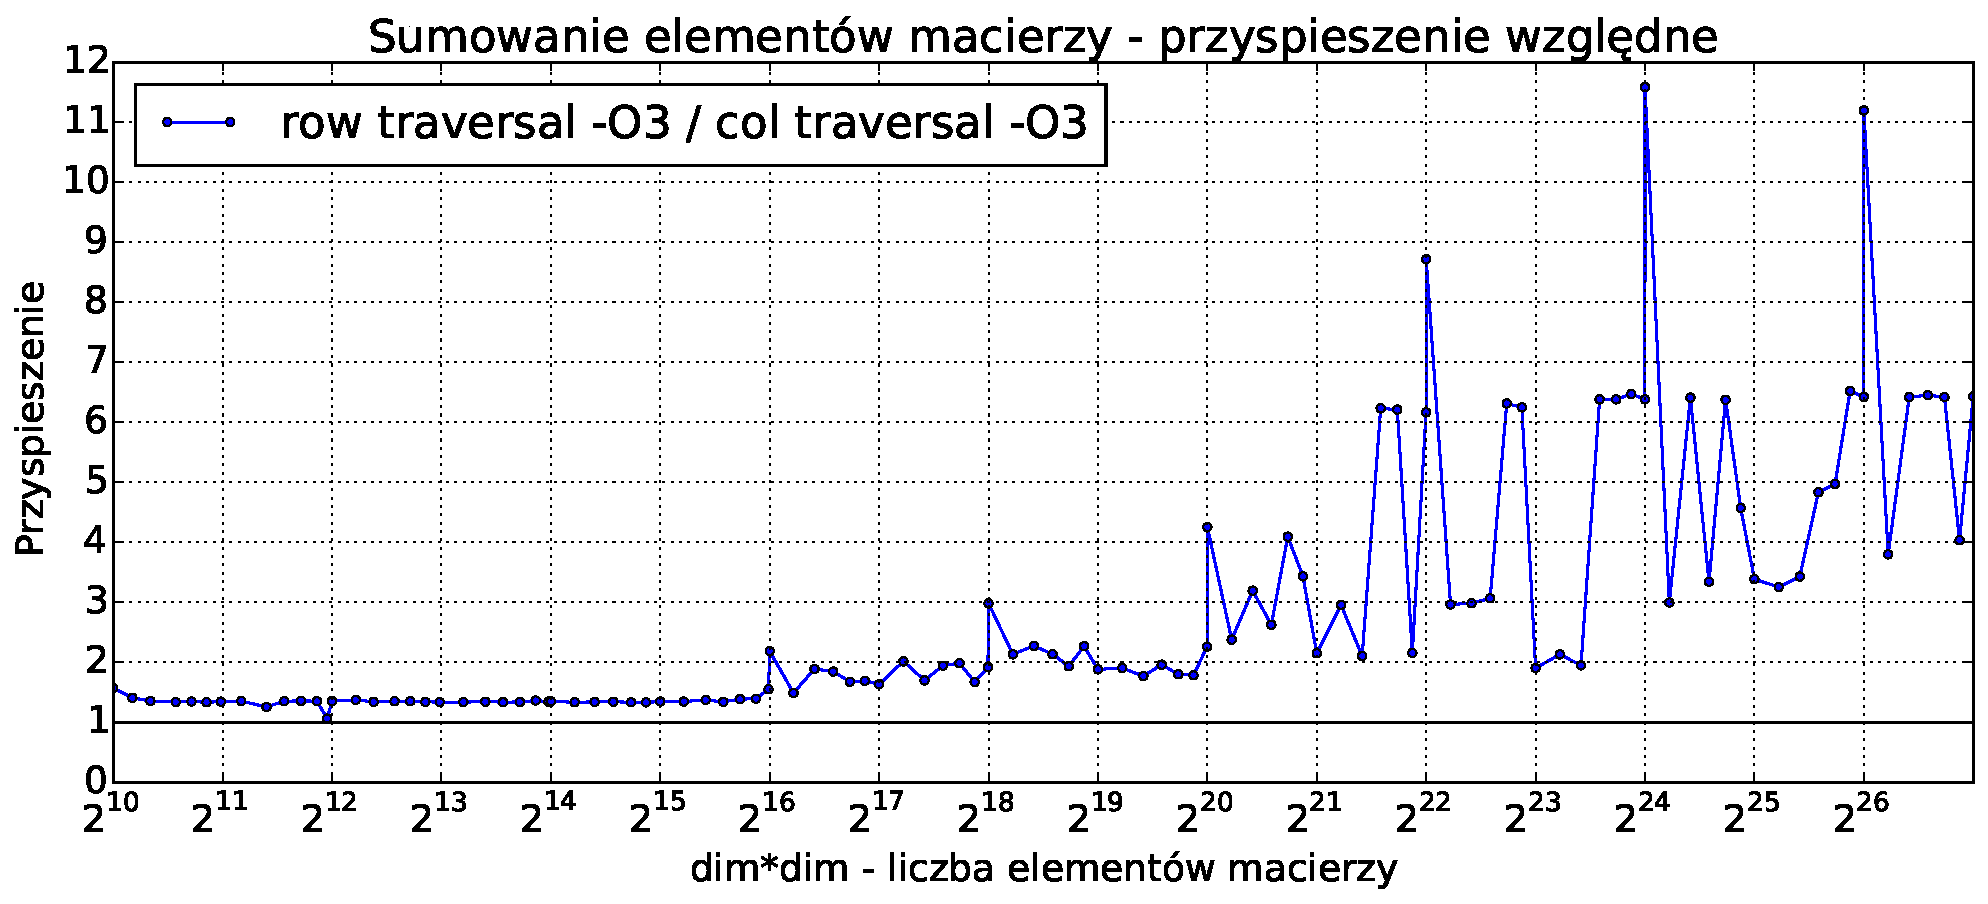
\includegraphics[width=0.80\textwidth]{images/benchs/matrix_sum_normalized}
        \caption{Wydajność przejścia po wierszach względem przejścia po kolumnach dla flagi \texttt{-O3}.}
    \end{subfigure}
	\caption{Wyniki testów sumowania elementów macierzy (z sekcji \ref{sub:matrixTraversal}), dla~procesora \mbox{Intel i7-4720HQ}.}
	\label{fig:matrixResults}
\end{figure}

\clearpage

\begin{figure}[!h]
    \centering
    \begin{subfigure}[c]{0.45\textwidth}
        \centering
        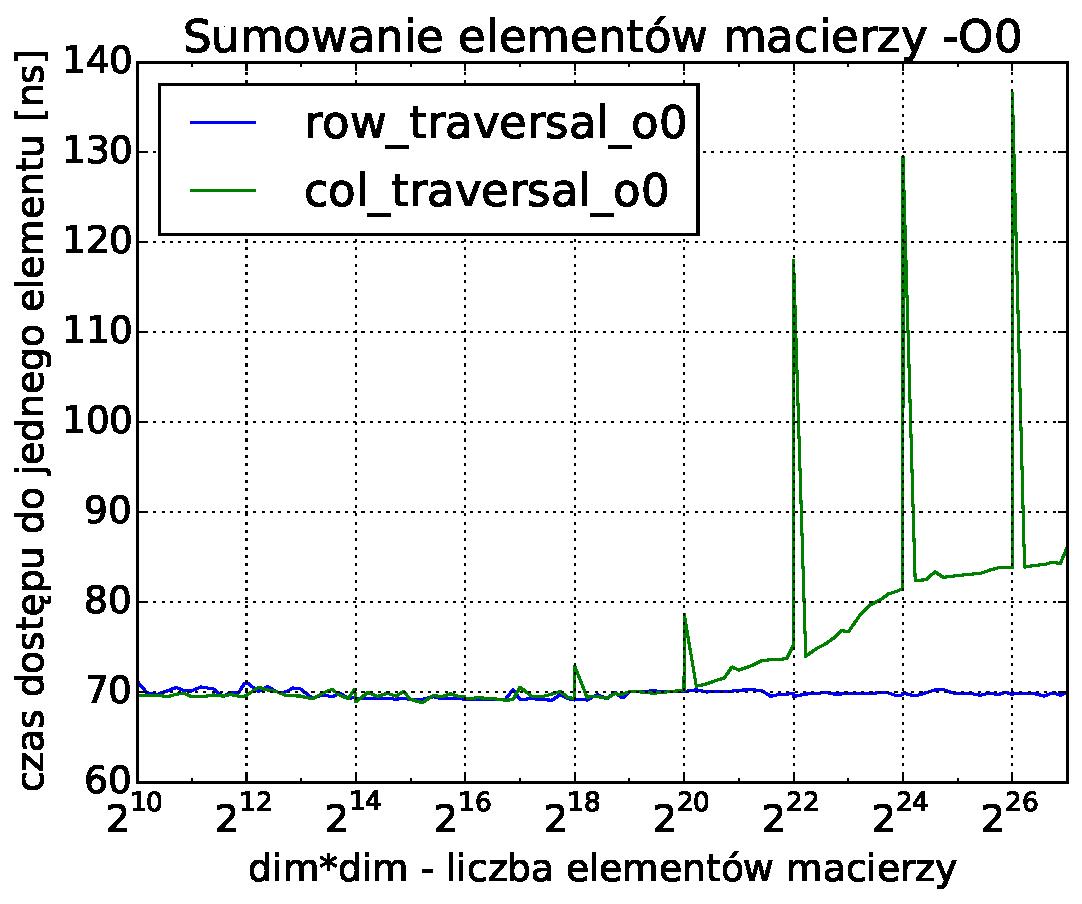
\includegraphics[width=\textwidth]{images/benchs_xeon/matrix_sum_O0}
        \caption{Kompilacja z flagą \texttt{-O0}}
    \end{subfigure}
    ~
    \begin{subfigure}[c]{0.45\textwidth}
        \centering
        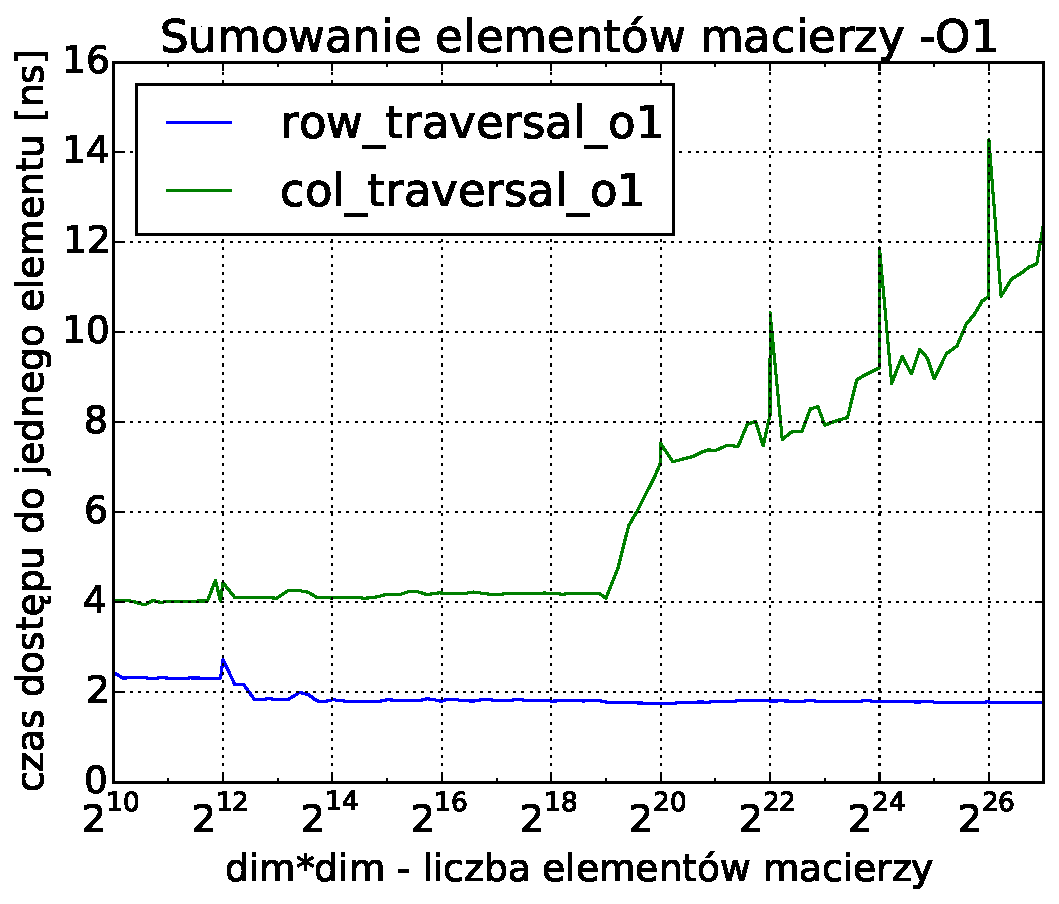
\includegraphics[width=\textwidth]{images/benchs_xeon/matrix_sum_O1}
        \caption{Kompilacja z flagą \texttt{-O1}}
    \end{subfigure}
    \\
    \vspace{0.4cm}
    \begin{subfigure}[c]{0.45\textwidth}
        \centering
        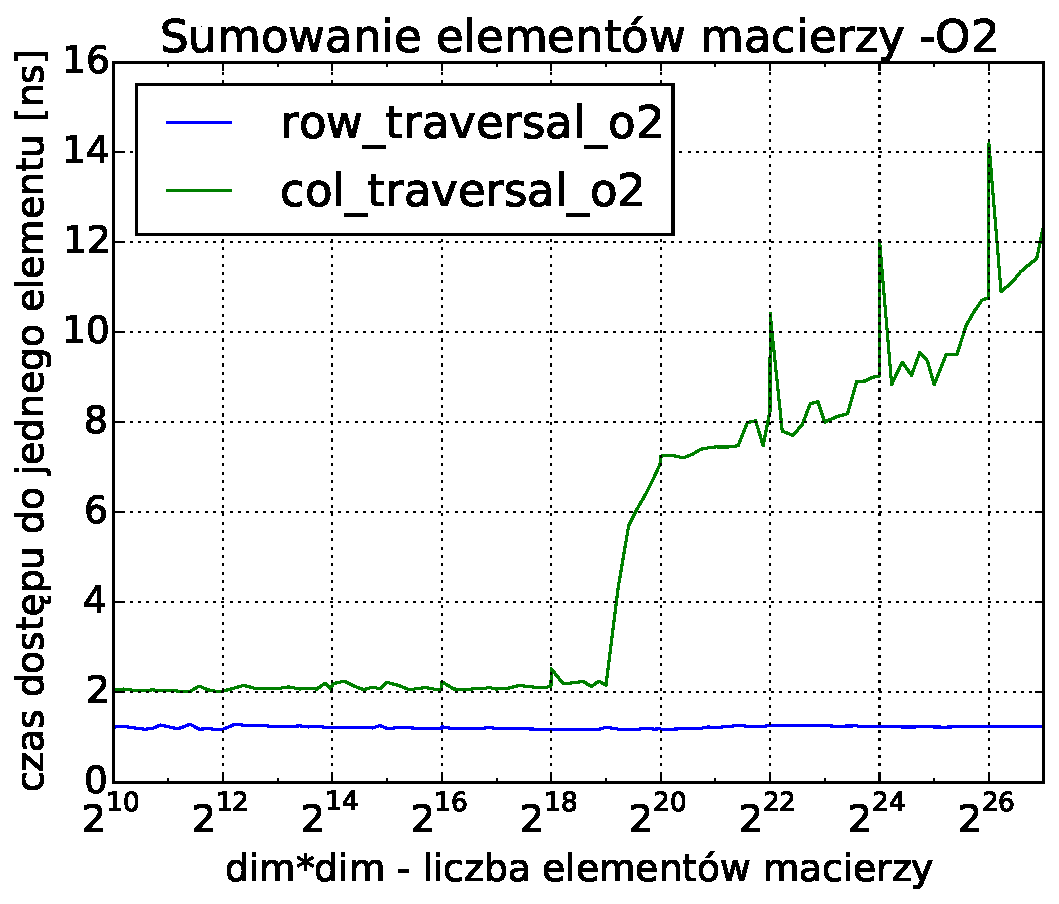
\includegraphics[width=\textwidth]{images/benchs_xeon/matrix_sum_O2}
        \caption{Kompilacja z flagą \texttt{-O2}}
    \end{subfigure}
    ~
    \begin{subfigure}[c]{0.45\textwidth}
        \centering
        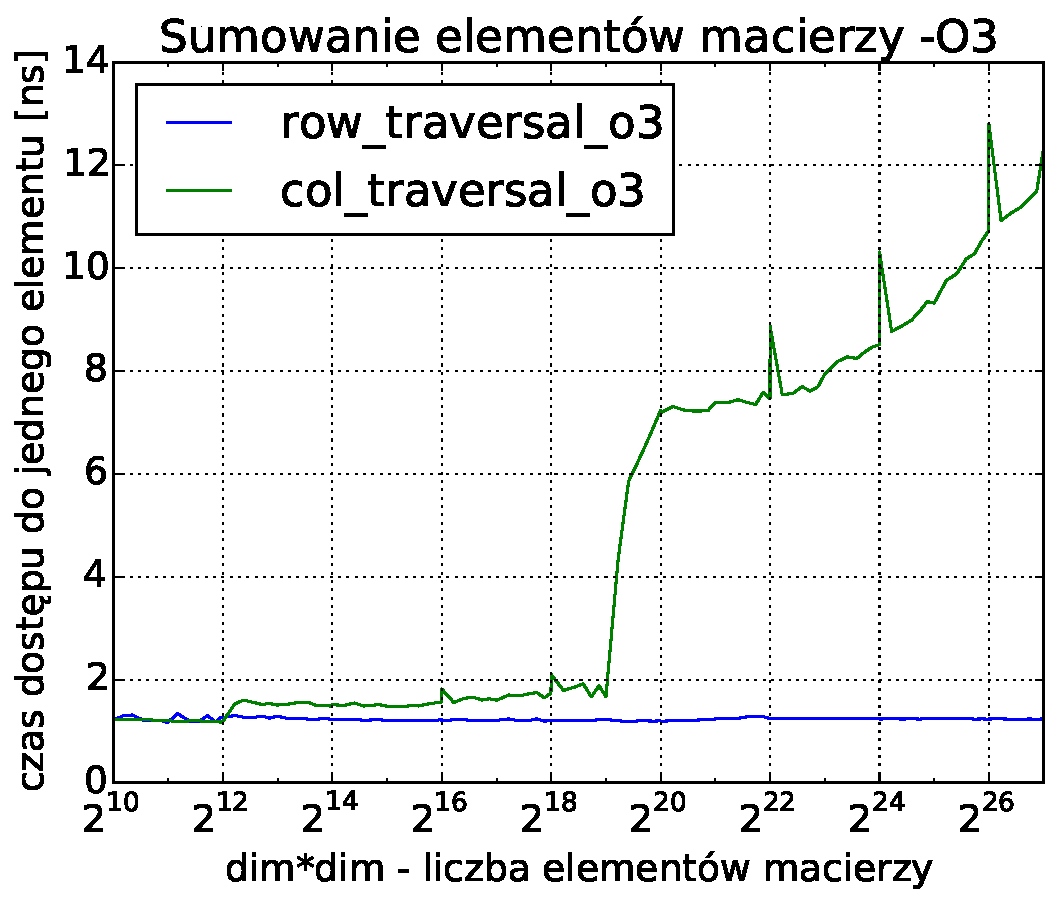
\includegraphics[width=\textwidth]{images/benchs_xeon/matrix_sum_O3}
        \caption{Kompilacja z flagą \texttt{-O3}}
    \end{subfigure}
    \\
    \vspace{0.4cm}
    \begin{subfigure}[c]{1.0\textwidth}
        \centering
        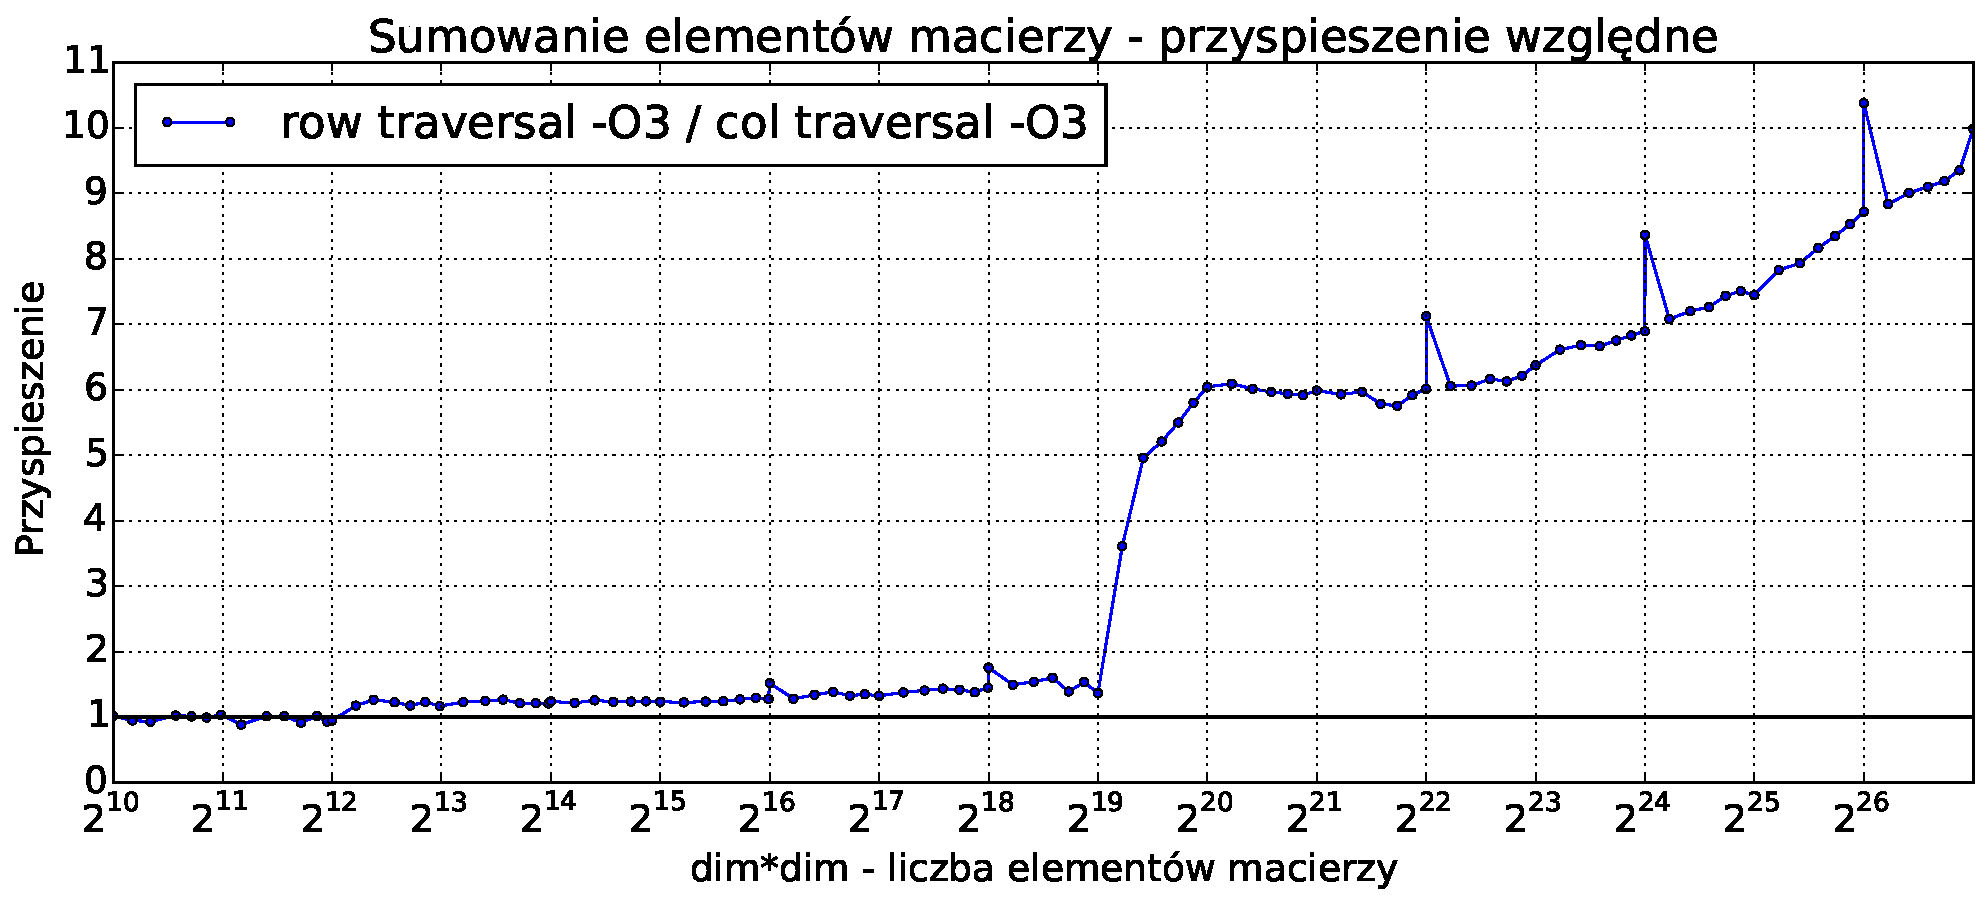
\includegraphics[width=0.80\textwidth]{images/benchs_xeon/matrix_sum_normalized}
        \caption{Wydajność przejścia po wierszach względem przejścia po kolumnach dla flagi \texttt{-O3}.}
        \label{fig:matrixResultsO3Xeon}
    \end{subfigure}
    \caption{Wyniki testów sumowania elementów macierzy (z sekcji \ref{sub:matrixTraversal}), dla~procesora \mbox{Intel Xeon W3565}.}
    \label{fig:matrixResultsXeon}
\end{figure}


\begin{table}[!h]
    \centering
    \caption{Statystyki programu perf dla problemu z sekcji \ref{sub:matrixTraversal} w wersji z optymalizacją \texttt{-O3}. W kolejnych komórkach znajdują się uśrednione statystyki z 20 przebiegów programu (flaga \texttt{$--$repeat} programu perf) dla wybranych rozmiarów macierzy oraz rodzaju przejścia. Na szaro oznaczono przejście kolumnami, a na biało wierszami.\\
        \textbf{1} -- liczba elementów macierzy oraz sposób przejścia po niej.\\
        \textbf{2} -- średni czas dostępu do jednego elementu [ns].\\
        \textbf{3} -- liczba wykonanych instrukcji.\\
        \textbf{4} -- liczba chybionych gałęzi (ang. \textit{branch misses}) [\%].\\
        \textbf{5} -- liczba chybień do cache L1d (danych) [\%].\\
        \textbf{6} -- liczba chybień do cache L3 [\%].\\}
    \label{tab:matrixSumPerf}
    \begin{tabular}{
        |l|S[table-format=2.2]|S[table-format=11.0]|S[table-format=2.2]|S[table-format=2.2]|S[table-format=2.2]|
    }
        \hline
        \multicolumn{1}{|c|}{\textbf{1}} & 
        \multicolumn{1}{|c|}{\textbf{2}} & 
        \multicolumn{1}{|c|}{\textbf{3}} & 
        \multicolumn{1}{|c|}{\textbf{4}} & 
        \multicolumn{1}{|c|}{\textbf{5}} & 
        \multicolumn{1}{|c|}{\textbf{6}}
         \\ \hline \hline
        $2^{20}$  & 0.6 & 528426650 & 0.05 & 6.26 & 12.76
        \\ \hline
        \rowcolor{lgray} $2^{20}$ & 3.01 & 692766880 & 0.04 & 99.55 & 6.62
        \\ \hline
        $2^{22}$  & 0.62 & 2129768639 & 0.02 & 6.35 & 53.32
        \\ \hline
        \rowcolor{lgray} $2^{22}$ & 7.14 & 2752463132 & 0.02 & 99.48 & 90.97
        \\ \hline
        $2^{23}$  & 0.61 & 4150161533 & 0.01 & 6.15 & 41.94
        \\ \hline
        \rowcolor{lgray} $2^{23}$ & 1.32 & 5527987761 & 0.01 & 98.52 & 98.08
        \\ \hline
        $2^{24}$  & 0.61 & 8614182665 & 0.01 & 6.11 & 38.47
        \\ \hline
        \rowcolor{lgray} $2^{24}$ & 8.79 & 11055702862 & 0.01 & 98.45 & 94.81
        \\ \hline
        $2^{25}$  & 0.61 & 17209919277 & 0.01 & 6.16 & 46.21
        \\ \hline
        \rowcolor{lgray} $2^{25}$ & 2.11 & 22291499139 & 0.0 & 96.18 & 6.64
        \\ \hline
        $2^{26}$  & 0.61 & 34382549263 & 0.0 & 6.43 & 44.93
        \\ \hline
        \rowcolor{lgray} $2^{26}$ & 8.58 & 44467984425 & 0.0 & 97.17 & 99.59
        \\ \hline
    \end{tabular}
\end{table}

\clearpage %TODO/FIXME
\section{Tablica struktur a struktura tablic}

Drugim zbadanym problemem jest organizacja danych w strukturach. Rozpatrzono trzy przypadki -- dostęp sekwencyjny, dostęp sekwencyjny z mniejszą strukturą danych oraz dostęp swobodny \cite{MindTheCache_AoSVsSoa, MindTheCache_CompactAoSVsSoa, MindTheCache_RandomAoSVsSoa}.

\subsection{Dostęp sekwencyjny}
\label{sub:aosVsSoaSequential}

W~poniższym przykładzie porównano czas wykonania prostego algorytmu, który polega na~zsumowaniu pozycji w trzech wymiarach (x, y, z). Na~listingach \ref{lst:aos} oraz \ref{lst:soa} przedstawiono dwa podejścia do~organizacji danych --~,,AoS'' (z~ang. \textit{array of structures}) --~tablica struktur oraz~,,SoA'' (z ang. \textit{structure of arrays}), czyli struktura tablic. Z~uwagi na~zmianę organizacji danych między przypadkami, sama implementacja algorytmu również uległa zmianie. Jego wynik jest~oczywiście taki sam w obu przypadkach.

\begin{lstlisting}[
    caption={Organizacja danych oraz implementacja algorytmu dla AoS.},
    label=lst:aos
]
struct particle {
    int x, y, z;
    int dx, dy, dz;
};
...
auto ps = create_particle_aos(n);

long int res = 0;			// testowany algorytm
for(const auto &particle: ps)
    res += particle.x + particle.y + particle.z;
return res;
\end{lstlisting}


\begin{lstlisting}[
    caption={Organizacja danych oraz implementacja algorytmu dla SoA.},
    label=lst:soa
]
struct particle_soa {
    std::vector<int> x, y, z;
    std::vector<int> dx, dy, dz;
};
...
auto ps = create_particle_soa(n);

long int res = 0;			// testowany algorytm
for (std::size_t i = 0; i < n; ++i)
    res += ps.x[i] + ps.y[i] + ps.z[i];
return res;
\end{lstlisting}

W tabelach \ref{tab:aosLayout} oraz \ref{tab:soaLayout} przedstawiono organizację obu struktur danych w trzech kolejnych liniach cache pobieranych przez procesor.


\begin{table}[!h]
    \centering
    \caption{Organizacja tablicy struktur (AoS) w kolejnych liniach cache pobieranych przez procesor dla algorytmu z listingu \ref{lst:aos}. Wiersze oznaczają linie cache (każda ma 64B). Na niebiesko zaznaczone zostały dane wykorzystywane przez algorytm, na szaro te, które są pobieranie niepotrzebnie.}
    \label{tab:aosLayout}
    \begin{tabular}{|0|0|0|0|0|0|0|0|0|0|0|0|0|0|0|0|}
        \hline
        \cellcolor{blueiii}x1 & \cellcolor{blueiii}y1 & \cellcolor{blueiii}z1 & \cellcolor{gray}dx1 & \cellcolor{gray}dy1 & \cellcolor{gray}dz1 & \cellcolor{blueiii}x2 & \cellcolor{blueiii}y2 & \cellcolor{blueiii}z2 & \cellcolor{gray}dx2 & \cellcolor{gray}dy2 & \cellcolor{gray}dz2 & \cellcolor{blueiii}x3 & \cellcolor{blueiii}y3 & \cellcolor{blueiii}z3 & \cellcolor{gray}dx3
        \\ \hline
        \cellcolor{gray}dy3 & \cellcolor{gray}dz3 & \cellcolor{blueiii}x4 & \cellcolor{blueiii}y4 & \cellcolor{blueiii}z4 & \cellcolor{gray}dx4 & \cellcolor{gray}dy4 & \cellcolor{gray}dz4 & \cellcolor{blueiii}x5 & \cellcolor{blueiii}y5 & \cellcolor{blueiii}z5 & \cellcolor{gray}dx5 & \cellcolor{gray}dy5 & \cellcolor{gray}dz5 & \cellcolor{blueiii}x6 & \cellcolor{blueiii}y6
        \\ \hline
        \cellcolor{blueiii}z6 & \cellcolor{gray}dx6 & \cellcolor{gray}dy6 & \cellcolor{gray}dz6 & \cellcolor{blueiii}x7 & \cellcolor{blueiii}y7 & \cellcolor{blueiii}z7 & \cellcolor{gray}dx7 & \cellcolor{gray}dy7 & \cellcolor{gray}dz7 & \cellcolor{blueiii}x8 & \cellcolor{blueiii}y8 & \cellcolor{blueiii}z8 & \cellcolor{gray}dx8 & \cellcolor{gray}dy8 & \cellcolor{gray}dz8
        \\ \hline
    \end{tabular}
\end{table}

\begin{table}[!h]
    \centering
    \caption{Organizacja struktury tablic (SoA) w kolejnych liniach cache. Wiersze oznaczają linie cache (każda ma 64B). Wszystkie dane znajdujące się w pobieranych liniach cache są wykorzystywane przez algorytm.}
    \label{tab:soaLayout}
    \begin{tabular}{|0|0|0|0|0|0|0|0|0|0|0|0|0|0|0|0|}
        \hline
        \cellcolor{blueiii}x1 & \cellcolor{blueiii}x2 & \cellcolor{blueiii}x3 & \cellcolor{blueiii}x4 & \cellcolor{blueiii}x5 & \cellcolor{blueiii}x6 & \cellcolor{blueiii}x7 & \cellcolor{blueiii}x8 & \cellcolor{blueiii}x9 & \cellcolor{blueiii}x10 & \cellcolor{blueiii}x11 & \cellcolor{blueiii}x12 & \cellcolor{blueiii}x13 & \cellcolor{blueiii}x14 & \cellcolor{blueiii}x15 & \cellcolor{blueiii}x16
        \\ \hline
        \cellcolor{blueiii}y1 & \cellcolor{blueiii}y2 & \cellcolor{blueiii}y3 & \cellcolor{blueiii}y4 & \cellcolor{blueiii}y5 & \cellcolor{blueiii}y6 & \cellcolor{blueiii}y7 & \cellcolor{blueiii}y8 & \cellcolor{blueiii}y9 & \cellcolor{blueiii}y10 & \cellcolor{blueiii}y11 & \cellcolor{blueiii}y12 & \cellcolor{blueiii}y13 & \cellcolor{blueiii}y14 & \cellcolor{blueiii}y15 & \cellcolor{blueiii}y16
        \\ \hline
        \cellcolor{blueiii}z1 & \cellcolor{blueiii}z2 & \cellcolor{blueiii}z3 & \cellcolor{blueiii}z4 & \cellcolor{blueiii}z5 & \cellcolor{blueiii}z6 & \cellcolor{blueiii}z7 & \cellcolor{blueiii}z8 & \cellcolor{blueiii}z9 & \cellcolor{blueiii}z10 & \cellcolor{blueiii}z11 & \cellcolor{blueiii}z12 & \cellcolor{blueiii}z13 & \cellcolor{blueiii}z14 & \cellcolor{blueiii}z15 & \cellcolor{blueiii}z16
        \\ \hline
    \end{tabular}
\end{table}

Implementacja AoS (z listingu \ref{lst:aos}) iteruje po kolejnych elementach tablicy struktur -- procesor widzi, że dostęp do danych odbywa się sekwencyjnie, więc pobiera kolejne dane. Problem tego rozwiązania polega na tym, że struktury (czyli wszystkie jej pola) są ułożone w pamięci sekwencyjnie. Zatem, aby~zsumować pozycję 16 cząsteczek, procesor musi skorzystać z 6 linii cache (bo jest w stanie pobierać dane tylko w formie bloków o rozmiarze linii cache -- czyli tutaj 64B).

Dla podejścia SoA (z listingu \ref{lst:soa}) algorytm iteruje po trzech wektorach równocześnie. Dzięki zmianie organizacji struktury na taką, która zawiera potrzebne elementy w osobnych tablicach, procesor nie~musi pobierać niepotrzebnych danych. Stąd, aby zsumować pozycję 16 elementów, wymagane są~tylko 3 linie cache.

Dla najbardziej agresywnej optymalizacji \texttt{-O3} podejście SoA jest około dwukrotnie szybsze (w~zależności od liczby elementów), co~widać na rysunku~\ref{fig:aosVsSoaSequential}. Wynika to~z~dwóch rzeczy. Po~pierwsze, w~podejściu AoS procesor pobiera więcej danych. Po~drugie, mechanizm wczesnego pobierania w przypadku SoA pobiera kolejne elementy wektorów \texttt{x}, \texttt{y} oraz \texttt{z} równolegle. Efekt ten widać również w kolejnej sekcji (\ref{sub:compactAosVsSoa}) -- gdzie ze struktury wyrzucono niewykorzystywane dane.


Na rysunku \ref{fig:aosVsSoaSequentialXeon} przedstawiono wyniki testów dla procesora Intel Xeon W3565. Jak można zauważyć, uzyskane przyspieszenia są bardzo zbliżone.

\begin{figure}
    \centering
    \begin{subfigure}[c]{0.45\textwidth}
        \centering
        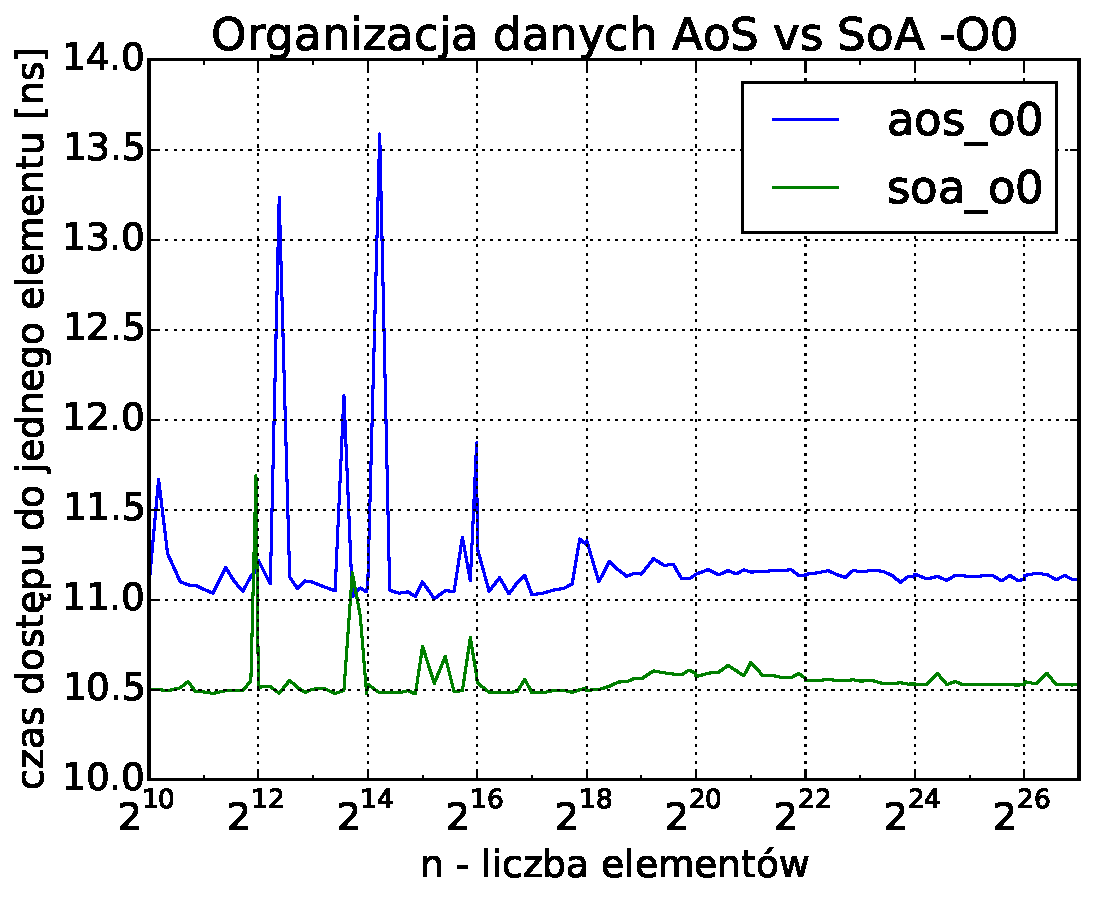
\includegraphics[width=\textwidth]{images/benchs/aos_vs_soa_O0}
        \caption{Kompilacja z flagą \texttt{-O0}}
    \end{subfigure}
    ~
    \begin{subfigure}[c]{0.45\textwidth}
        \centering
        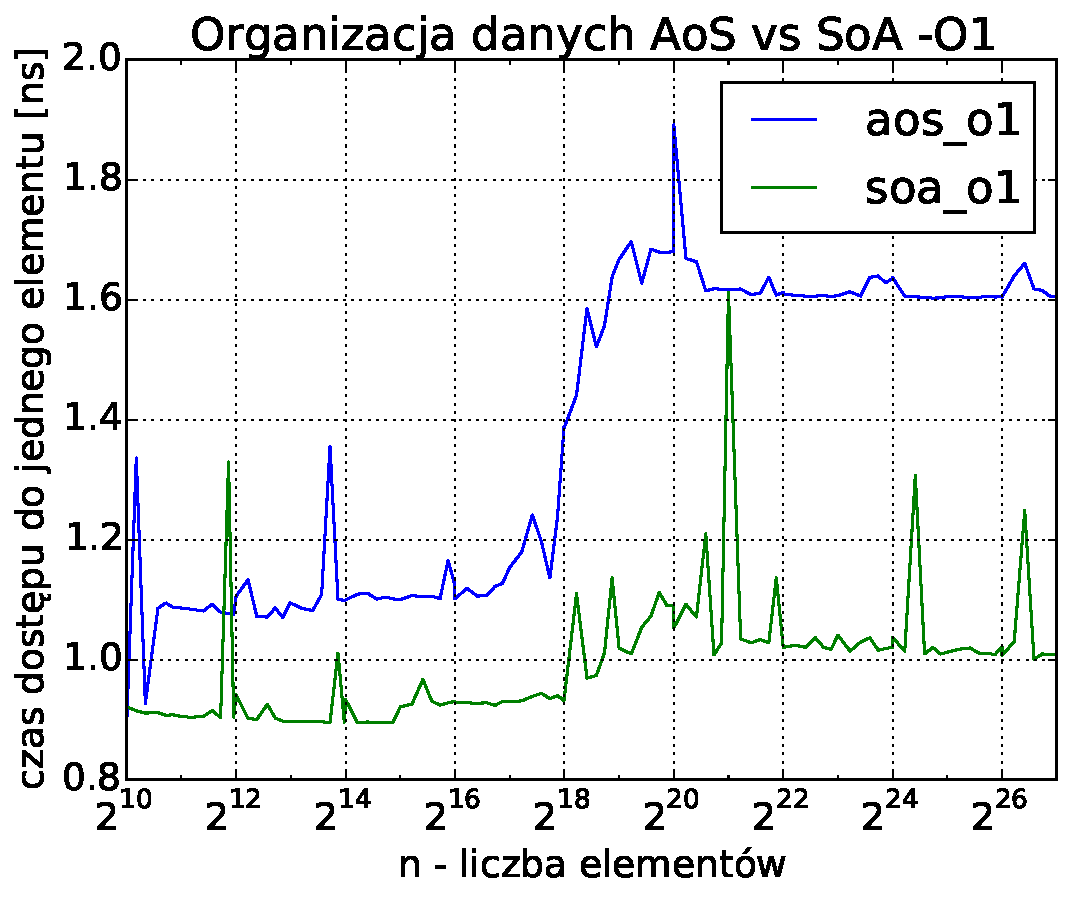
\includegraphics[width=\textwidth]{images/benchs/aos_vs_soa_O1}
        \caption{Kompilacja z flagą \texttt{-O1}}
    \end{subfigure}
    \\
    \vspace{0.55cm}
    \begin{subfigure}[c]{0.45\textwidth}
        \centering
        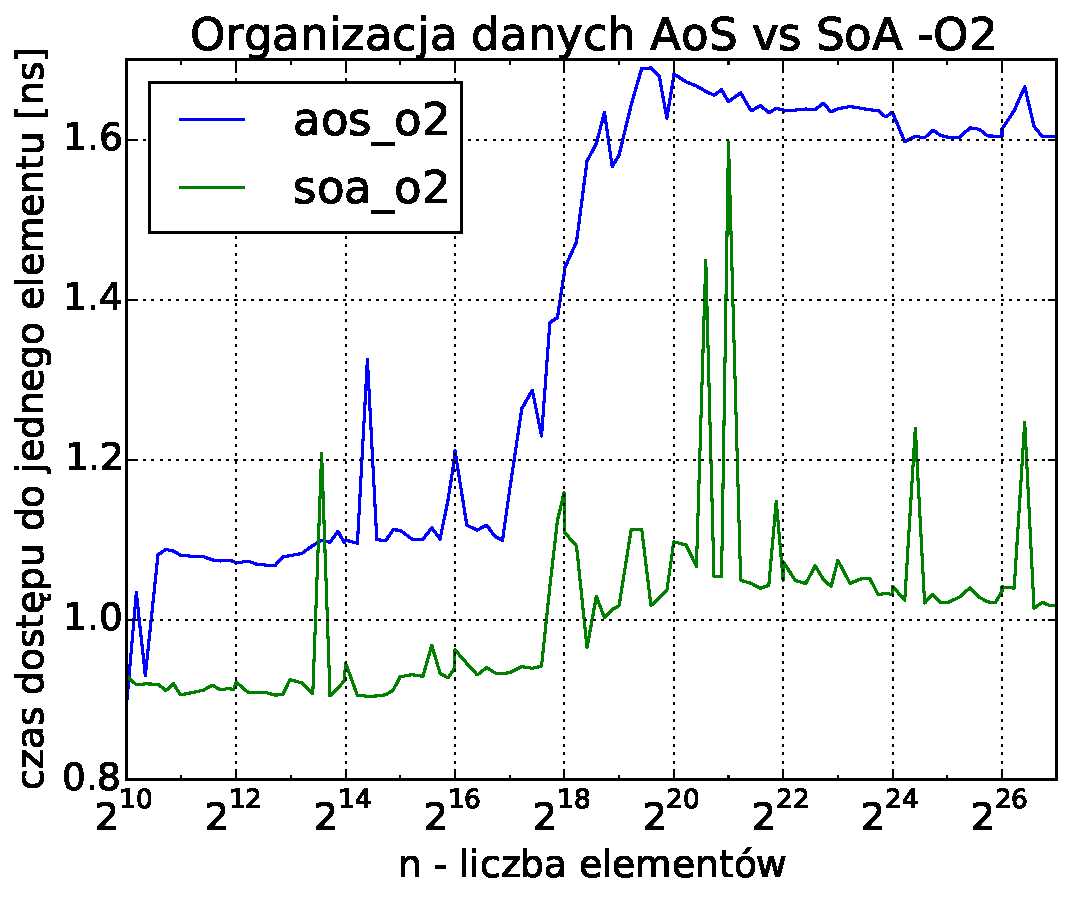
\includegraphics[width=\textwidth]{images/benchs/aos_vs_soa_O2}
        \caption{Kompilacja z flagą \texttt{-O2}}
    \end{subfigure}
    ~
    \begin{subfigure}[c]{0.45\textwidth}
        \centering
        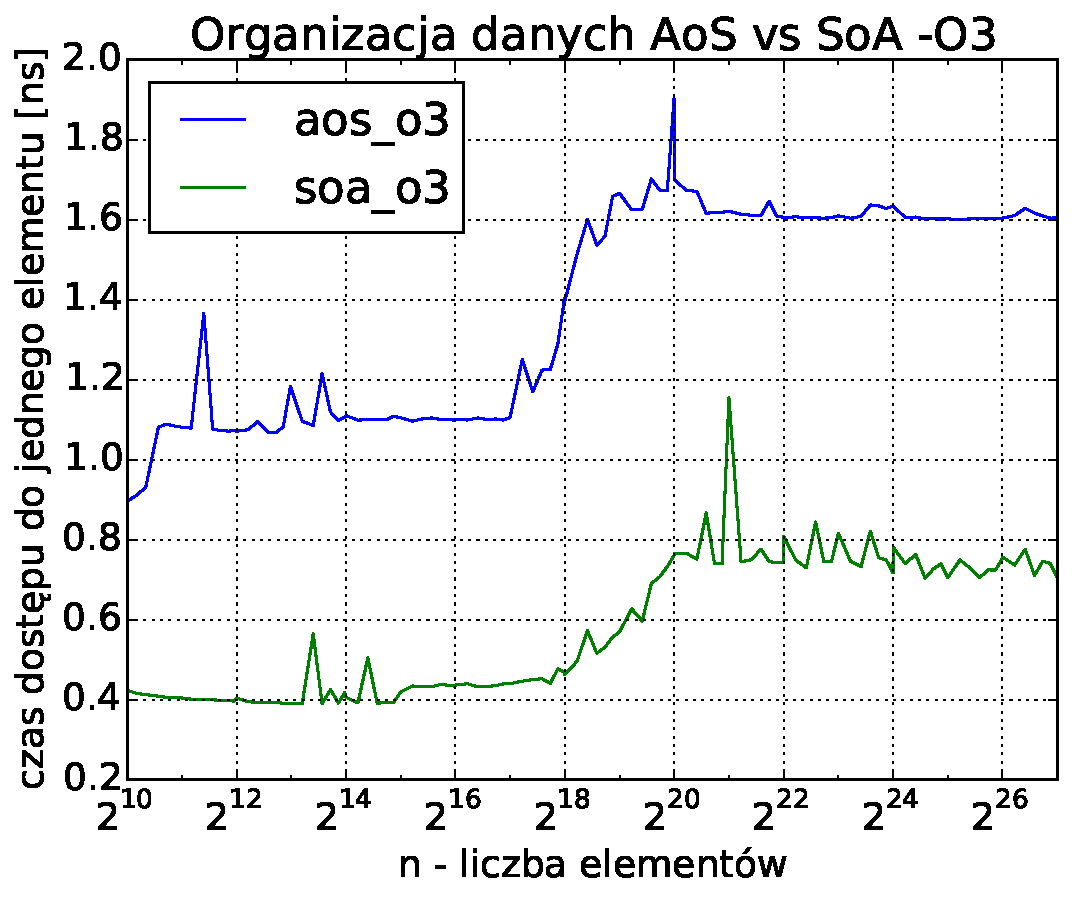
\includegraphics[width=\textwidth]{images/benchs/aos_vs_soa_O3}
        \caption{Kompilacja z flagą \texttt{-O3}}
    \end{subfigure}
    \\
    \vspace{0.55cm}
    \begin{subfigure}[c]{1.0\textwidth}
        \centering
        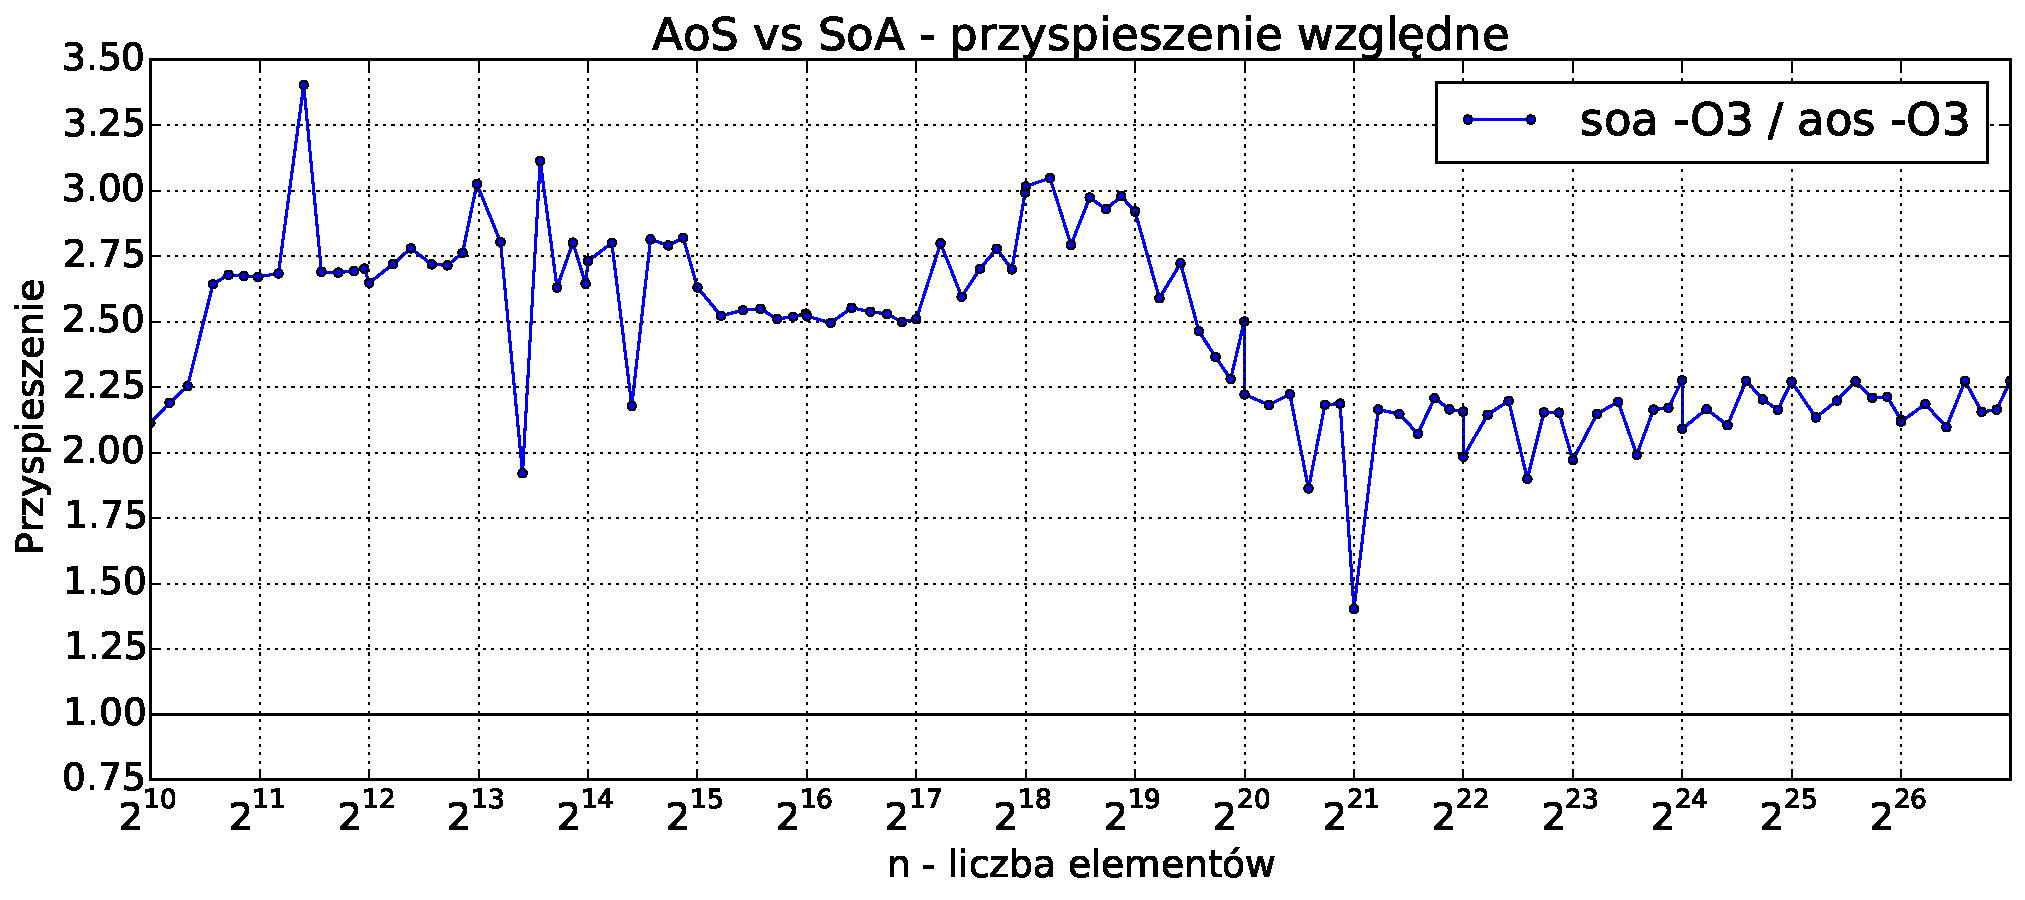
\includegraphics[width=0.80\textwidth]{images/benchs/aos_vs_soa_normalized}
        \caption{Wydajność SoA względem AoS dla flagi \texttt{-O3}.}
    \end{subfigure}
    \caption{Wyniki testów AoS vs SoA (z sekcji \ref{sub:aosVsSoaSequential}), dla~procesora \mbox{Intel i7-4720HQ}.}
    \label{fig:aosVsSoaSequential}
\end{figure}

\begin{figure}
    \centering
    \begin{subfigure}[c]{0.45\textwidth}
        \centering
        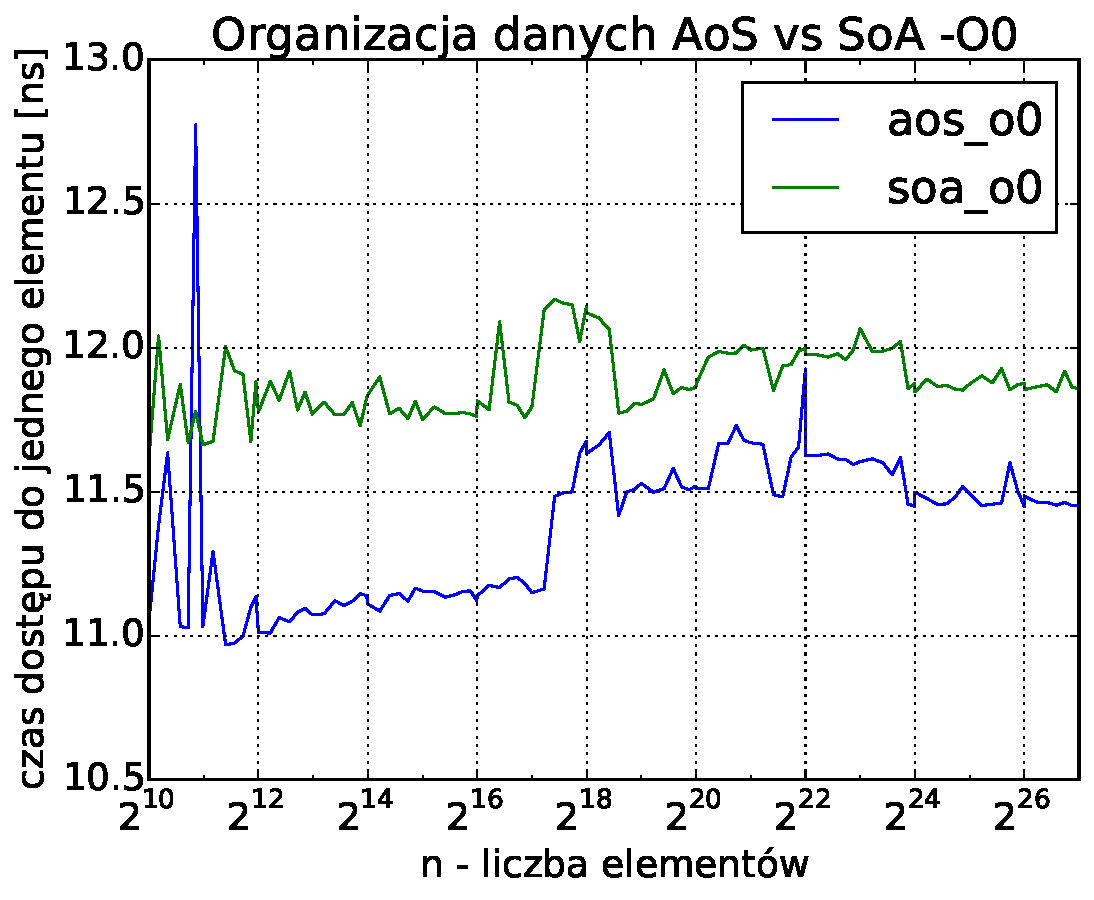
\includegraphics[width=\textwidth]{images/benchs_xeon/aos_vs_soa_O0}
        \caption{Kompilacja z flagą \texttt{-O0}}
    \end{subfigure}
    ~
    \begin{subfigure}[c]{0.45\textwidth}
        \centering
        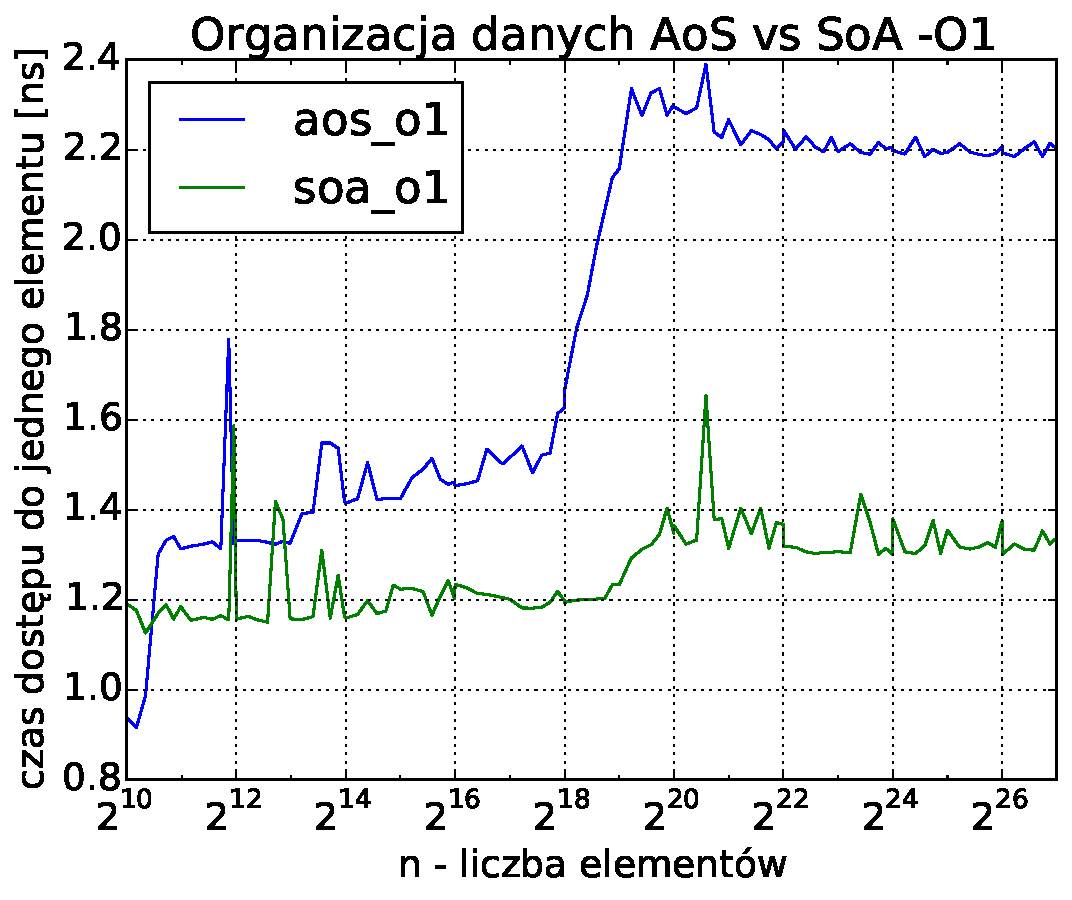
\includegraphics[width=\textwidth]{images/benchs_xeon/aos_vs_soa_O1}
        \caption{Kompilacja z flagą \texttt{-O1}}
    \end{subfigure}
    \\
    \vspace{0.55cm}
    \begin{subfigure}[c]{0.45\textwidth}
        \centering
        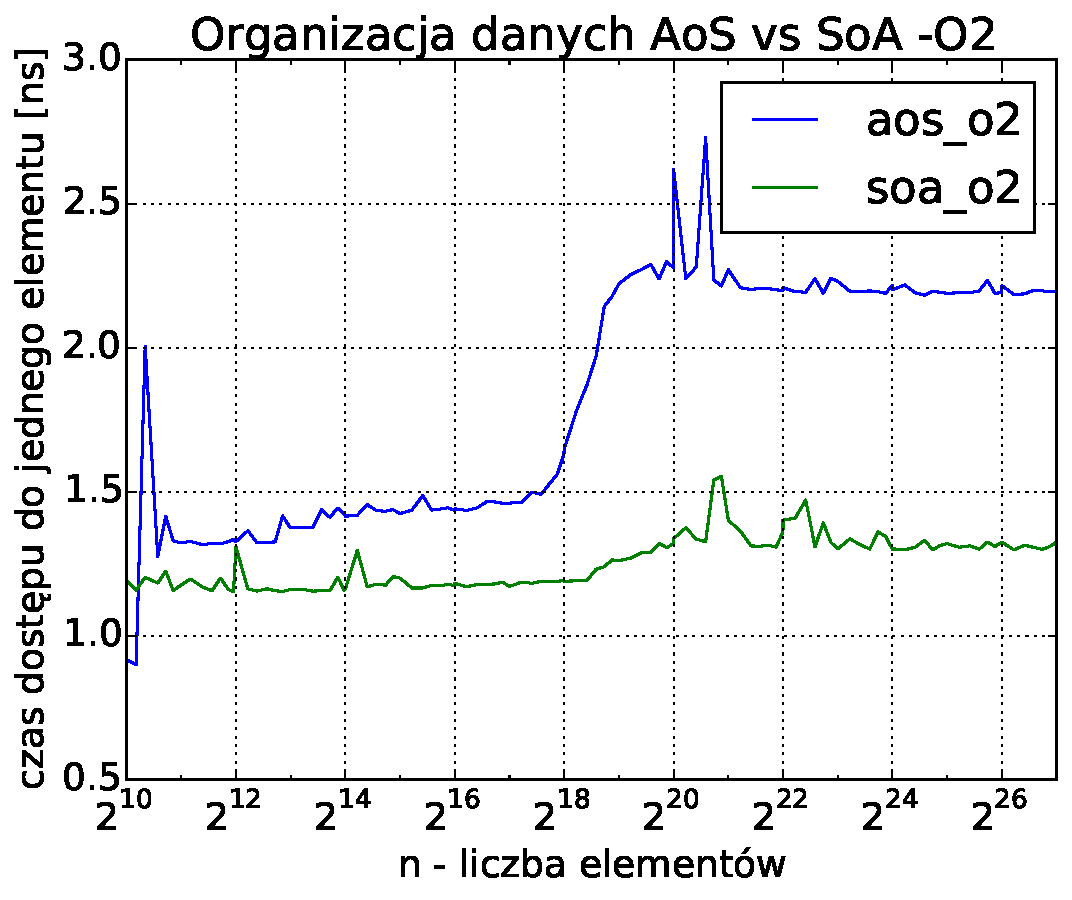
\includegraphics[width=\textwidth]{images/benchs_xeon/aos_vs_soa_O2}
        \caption{Kompilacja z flagą \texttt{-O2}}
    \end{subfigure}
    ~
    \begin{subfigure}[c]{0.45\textwidth}
        \centering
        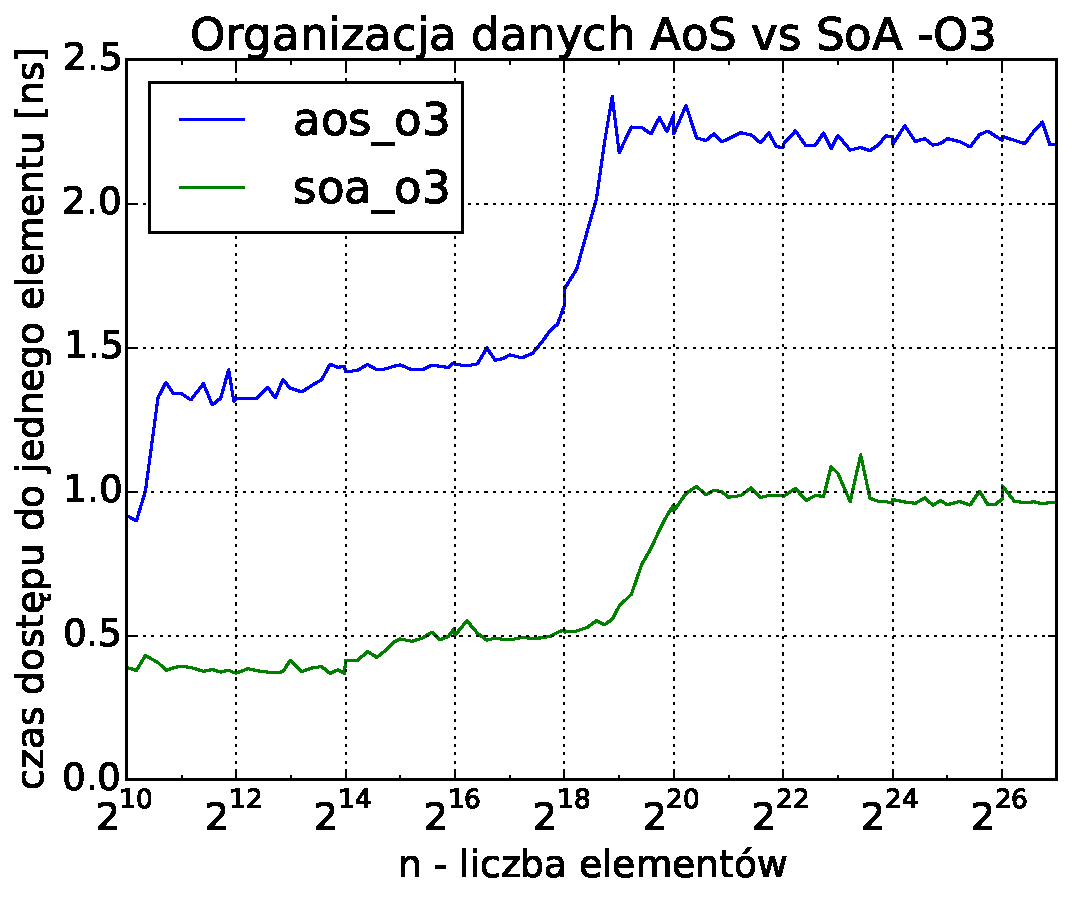
\includegraphics[width=\textwidth]{images/benchs_xeon/aos_vs_soa_O3}
        \caption{Kompilacja z flagą \texttt{-O3}}
    \end{subfigure}
    \\
    \vspace{0.55cm}
    \begin{subfigure}[c]{1.0\textwidth}
        \centering
        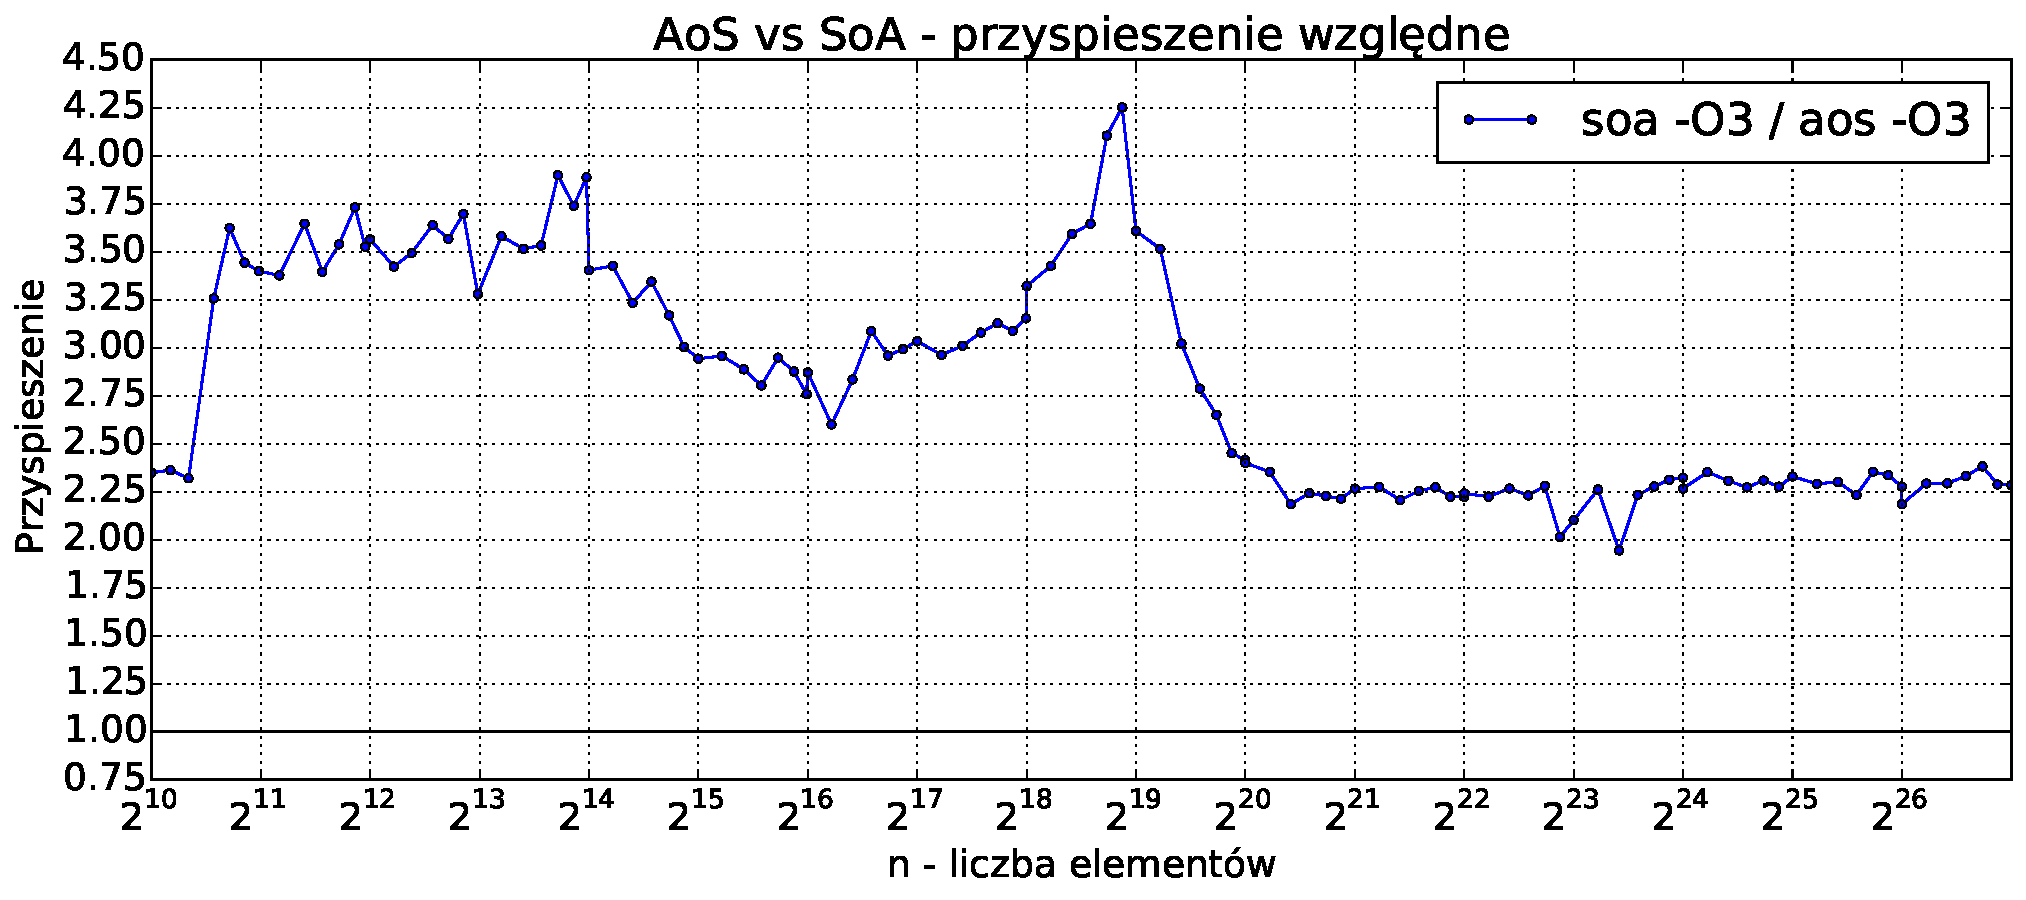
\includegraphics[width=0.80\textwidth]{images/benchs_xeon/aos_vs_soa_normalized}
        \caption{Wydajność SoA względem AoS dla flagi \texttt{-O3}.}
    \end{subfigure}
    \caption{Wyniki testów AoS vs SoA (z sekcji \ref{sub:aosVsSoaSequential}), dla~procesora Intel \mbox{Xeon W3565}.}
    \label{fig:aosVsSoaSequentialXeon}
\end{figure}

\clearpage

\subsection{Dostęp sekwencyjny -- ,,kompaktowa'' struktura}
\label{sub:compactAosVsSoa}
W kolejnym przykładzie ze struktur AoS oraz SoA usunięto dane niewykorzystywane przez opisany w sekcji \ref{sub:aosVsSoaSequential} algorytm (pola \texttt{dx}, \texttt{dy} oraz \texttt{dz}). Struktury te w ,,kompaktowej'' wersji przedstawiono na~listingach \ref{lst:compactAos} oraz \ref{lst:compactSoa}.

\begin{lstlisting}[
    caption={Organizacja danych kompaktowej struktury dla AoS.},
    label=lst:compactAos
]
struct particle {
    int x, y, z;
};
\end{lstlisting}
\begin{lstlisting}[
    caption={Organizacja danych kompaktowej struktury dla SoA.},
    label=lst:compactSoa
]
struct particle_soa {
    std::vector<int> x, y, z;
};
\end{lstlisting}

Na rysunku \ref{fig:compactAosLayout} przedstawiono wyniki. Jak można zauważyć, dla najbardziej agresywnej optymalizacji,  gdy ilość danych nie przekracza około 1 MB (czyli \textit{n} równe $2^{18}$), wciąż przyspieszenie jest znaczące -- około dwukrotne. Po przekroczeniu tego progu, z~uwagi na współdzielenie pamięci podręcznej L3, przyspieszenie nie jest tak duże -- spada do około 30\%, co~widać na~rysunku~\ref{fig:compactAosVsSoaRelative}.

Dla procesora Intel Xeon W3565 sytuacja wygląda podobnie, co widać na rysunku \ref{fig:compactAosLayoutXeon}. Zauważalną różnicą jest większy spadek przyspieszenia po~przekroczeniu rozmiaru pamięci podręcznej L2 --~czyli~ponad $2^{14}$ elementów. Wynika on stąd, że procesor Intel Xeon W3565 posiada większą pamięć podręczną L3 (8 MB), niż procesor Intel i7-4720HQ (6 MB), przez co dostęp do niej jest wolniejszy.

\begin{figure}
    \centering
    \begin{subfigure}[c]{0.45\textwidth}
        \centering
        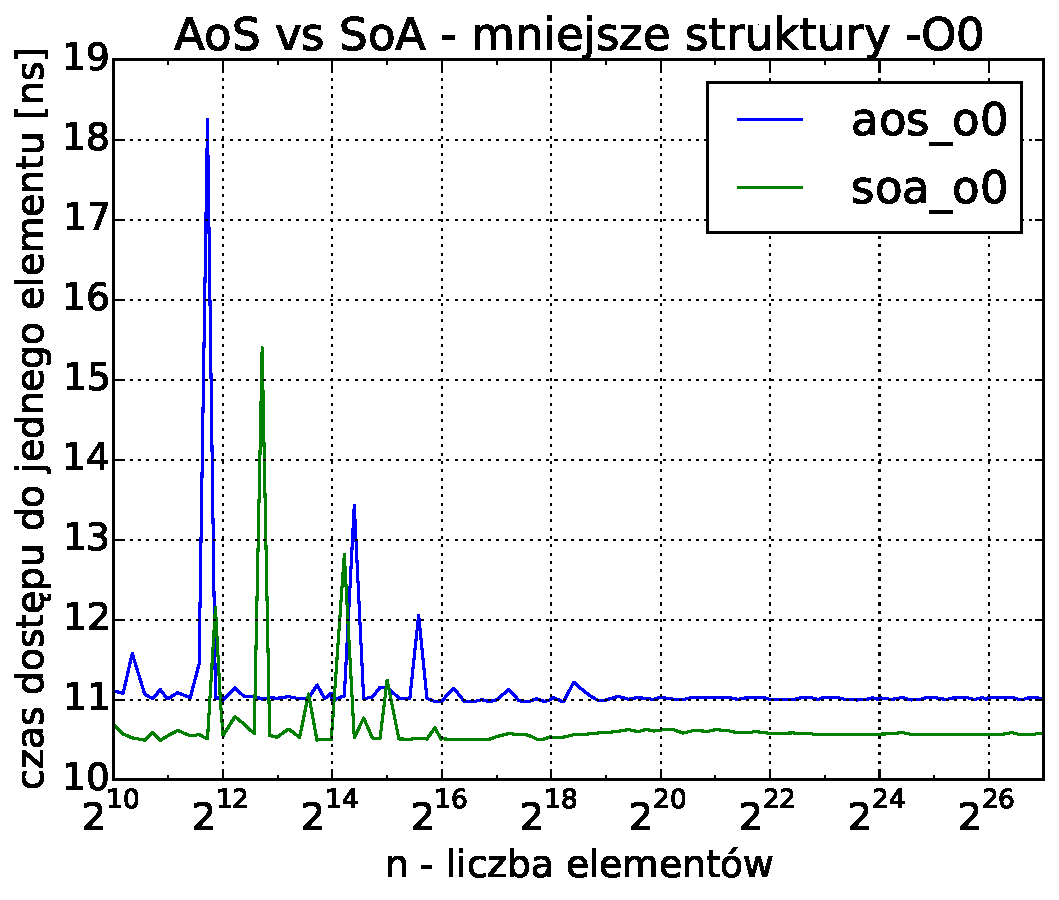
\includegraphics[width=\textwidth]{images/benchs/compact_aos_vs_soa_O0}
        \caption{Kompilacja z flagą \texttt{-O0}}
    \end{subfigure}
    ~
    \begin{subfigure}[c]{0.45\textwidth}
        \centering
        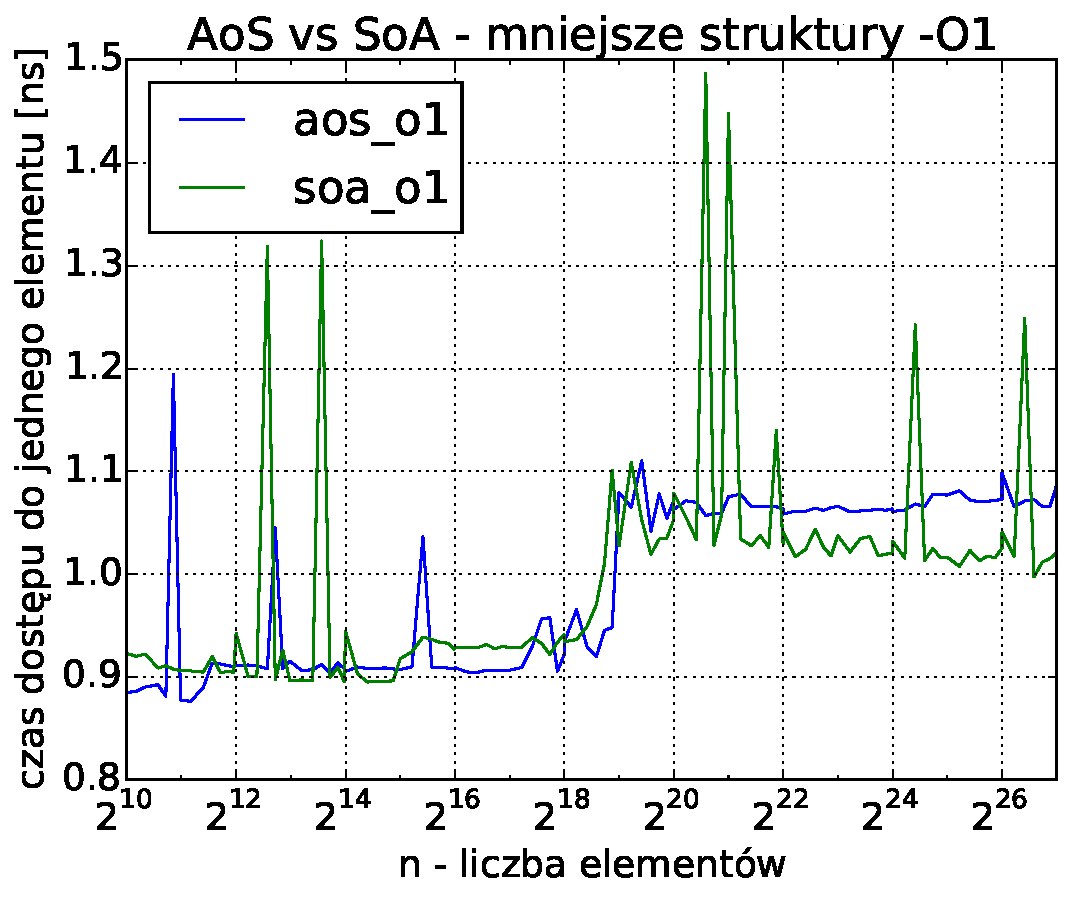
\includegraphics[width=\textwidth]{images/benchs/compact_aos_vs_soa_O1}
        \caption{Kompilacja z flagą \texttt{-O1}}
    \end{subfigure}
    \\
    \vspace{0.55cm}
    \begin{subfigure}[c]{0.45\textwidth}
        \centering
        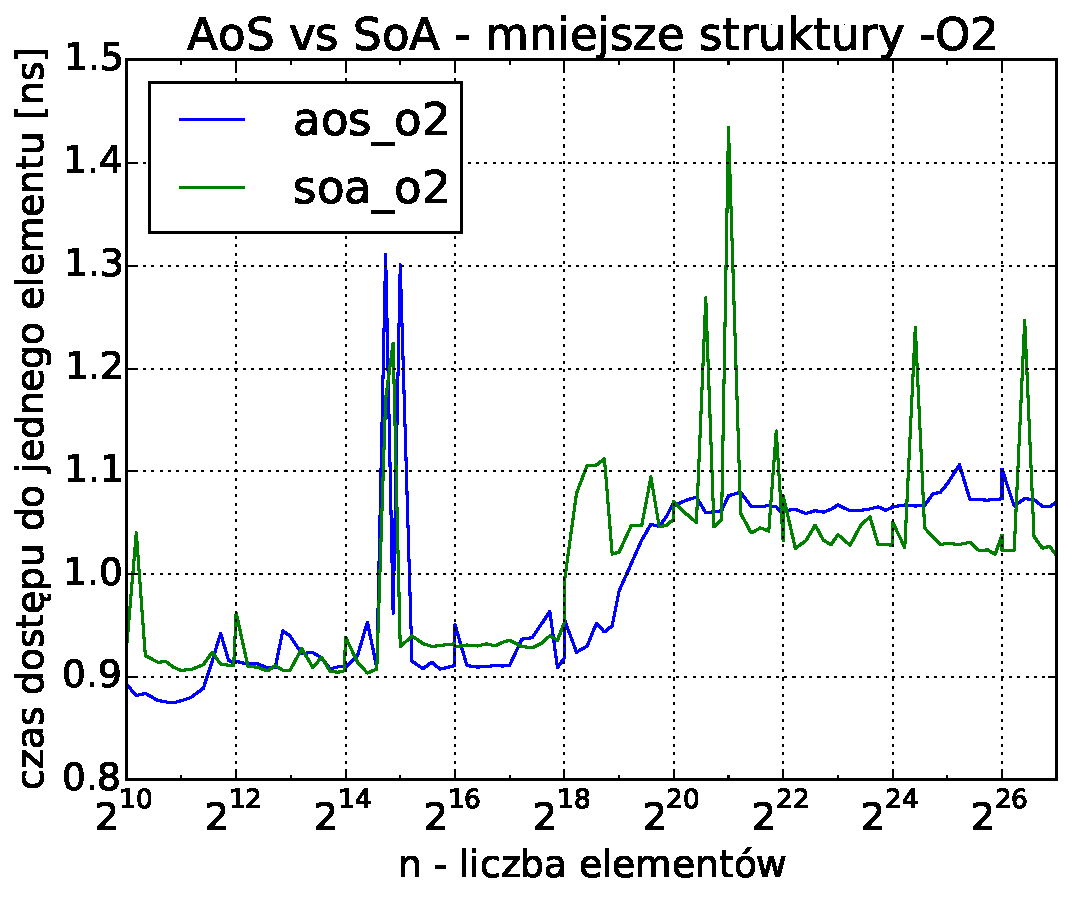
\includegraphics[width=\textwidth]{images/benchs/compact_aos_vs_soa_O2}
        \caption{Kompilacja z flagą \texttt{-O2}}
    \end{subfigure}
    ~
    \begin{subfigure}[c]{0.45\textwidth}
        \centering
        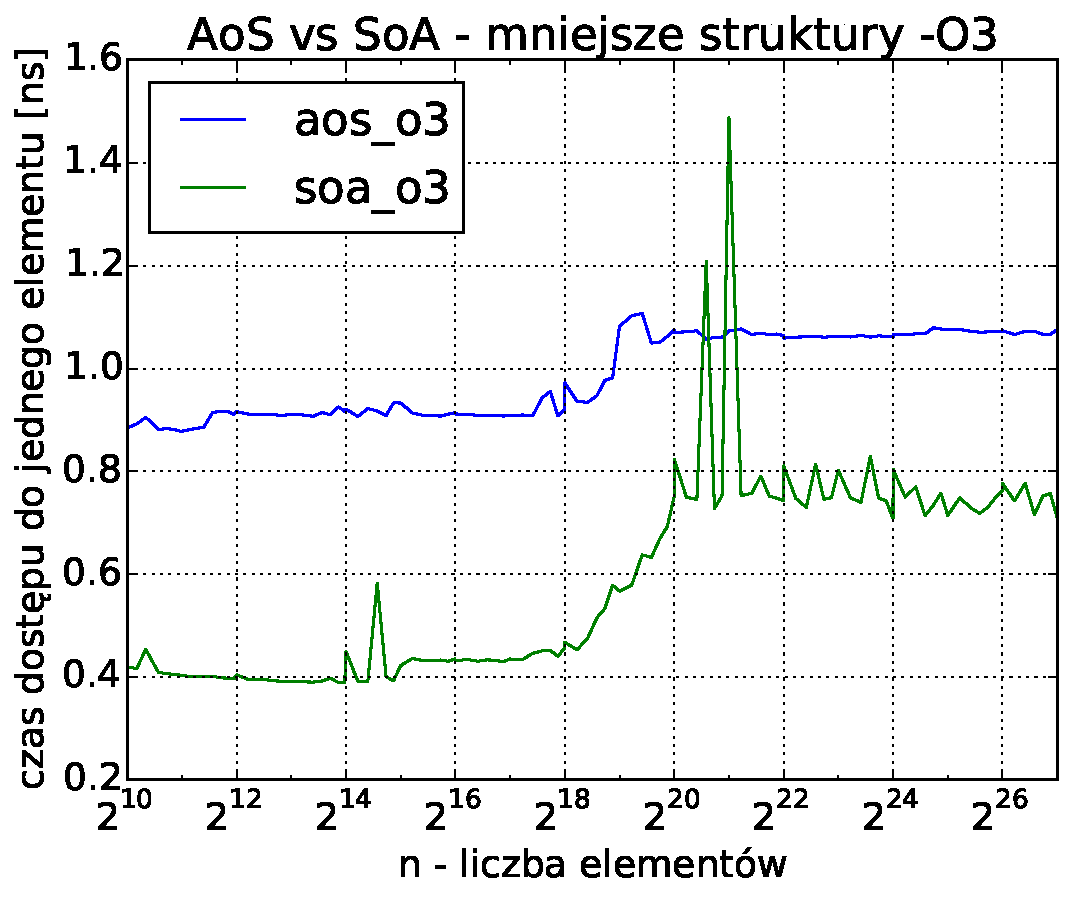
\includegraphics[width=\textwidth]{images/benchs/compact_aos_vs_soa_O3}
        \caption{Kompilacja z flagą \texttt{-O3}}
    \end{subfigure}
     \\
     \vspace{0.55cm}
     \begin{subfigure}[c]{1.0\textwidth}
         \centering
         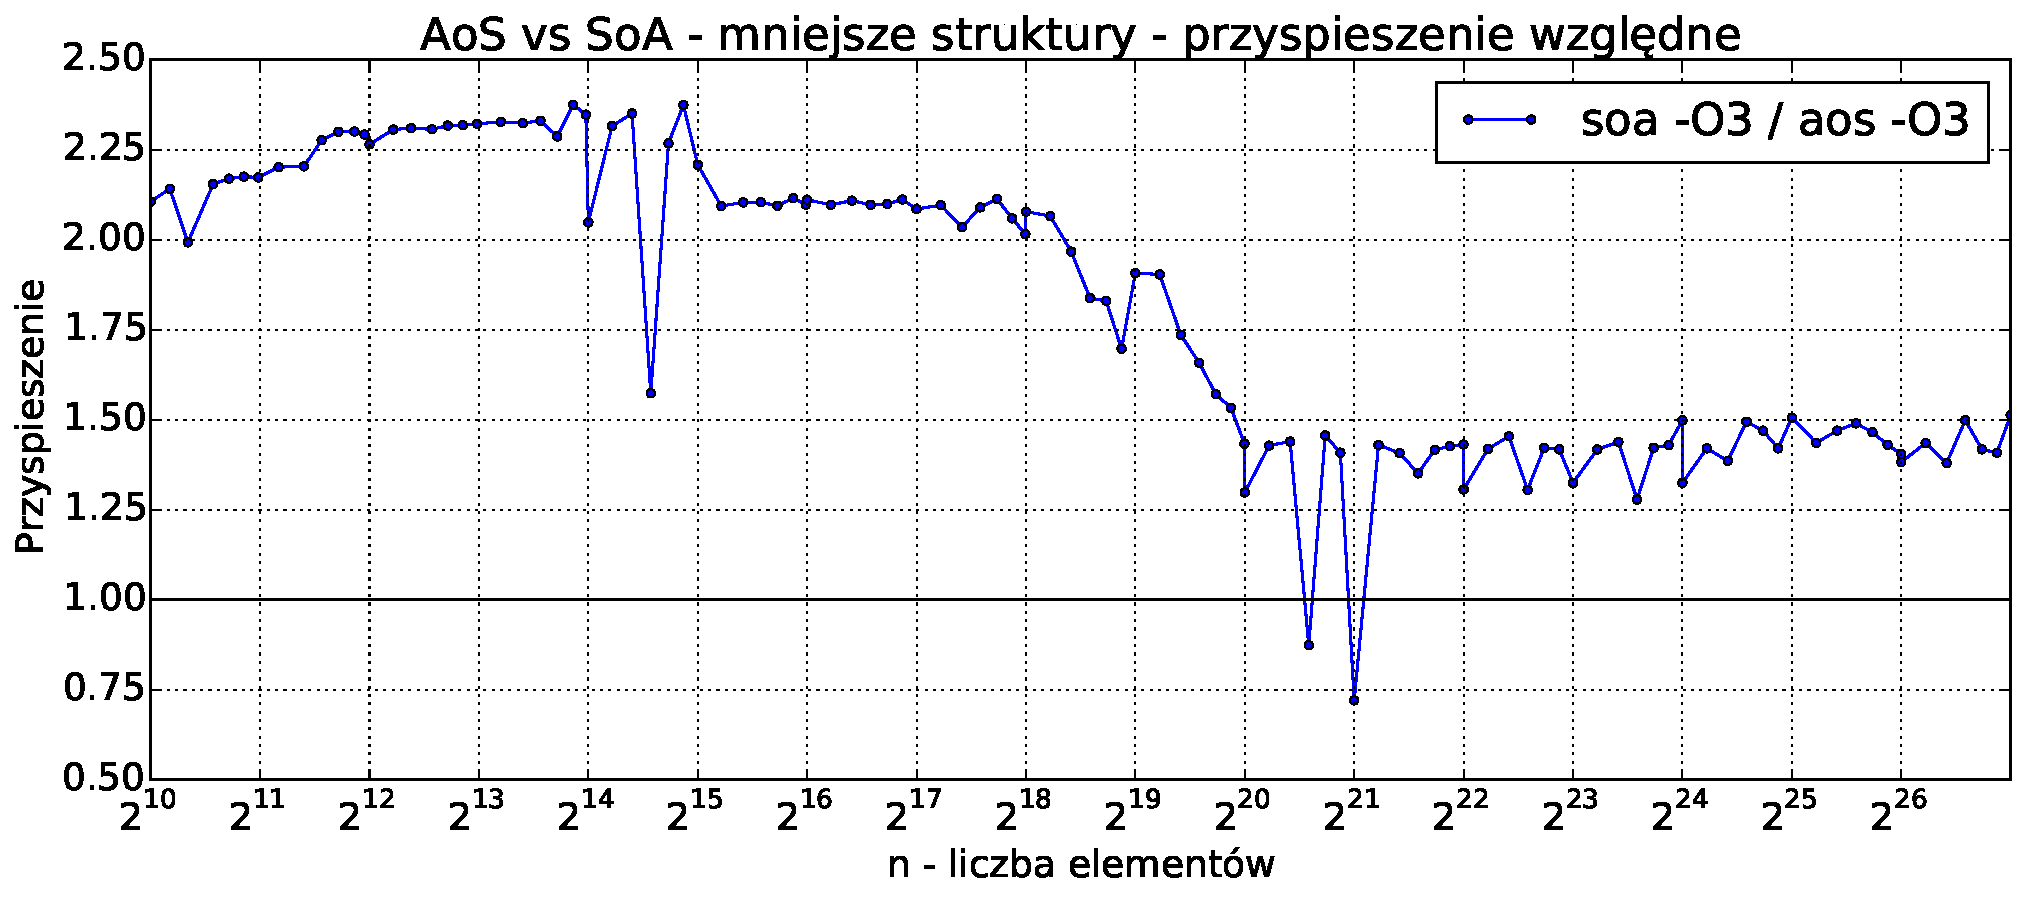
\includegraphics[width=0.80\textwidth]{images/benchs/compact_aos_vs_soa_normalized}
         \caption{Wydajność SoA względem AoS dla mniejszych struktur, dla flagi \texttt{-O3}.}
         \label{fig:compactAosVsSoaRelative}
        \end{subfigure}
    \caption{Wyniki testów AoS vs SoA dla mniejszych struktur (z sekcji \ref{sub:compactAosVsSoa}), dla~procesora \mbox{Intel i7-4720HQ}.}
    \label{fig:compactAosLayout}
\end{figure}

\begin{figure}
    \centering
    \begin{subfigure}[c]{0.45\textwidth}
        \centering
        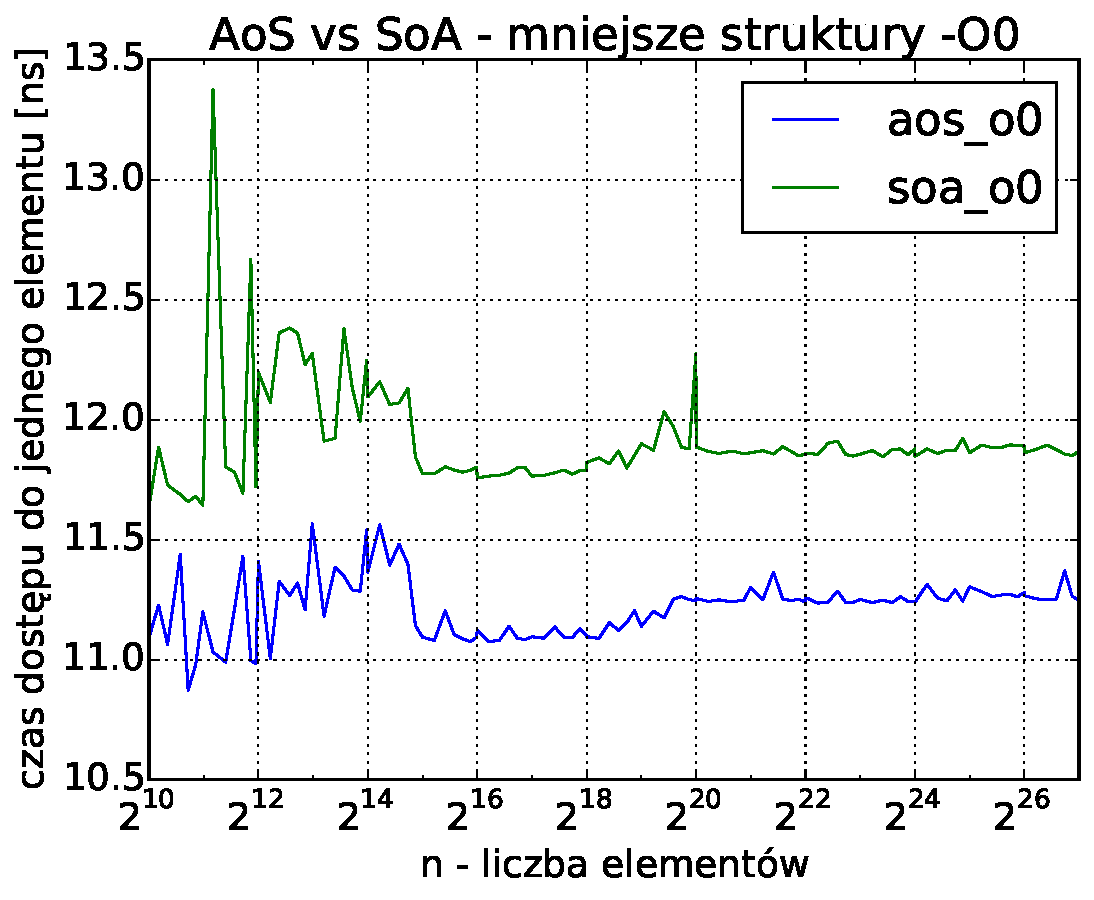
\includegraphics[width=\textwidth]{images/benchs_xeon/compact_aos_vs_soa_O0}
        \caption{Kompilacja z flagą \texttt{-O0}}
    \end{subfigure}
    ~
    \begin{subfigure}[c]{0.45\textwidth}
        \centering
        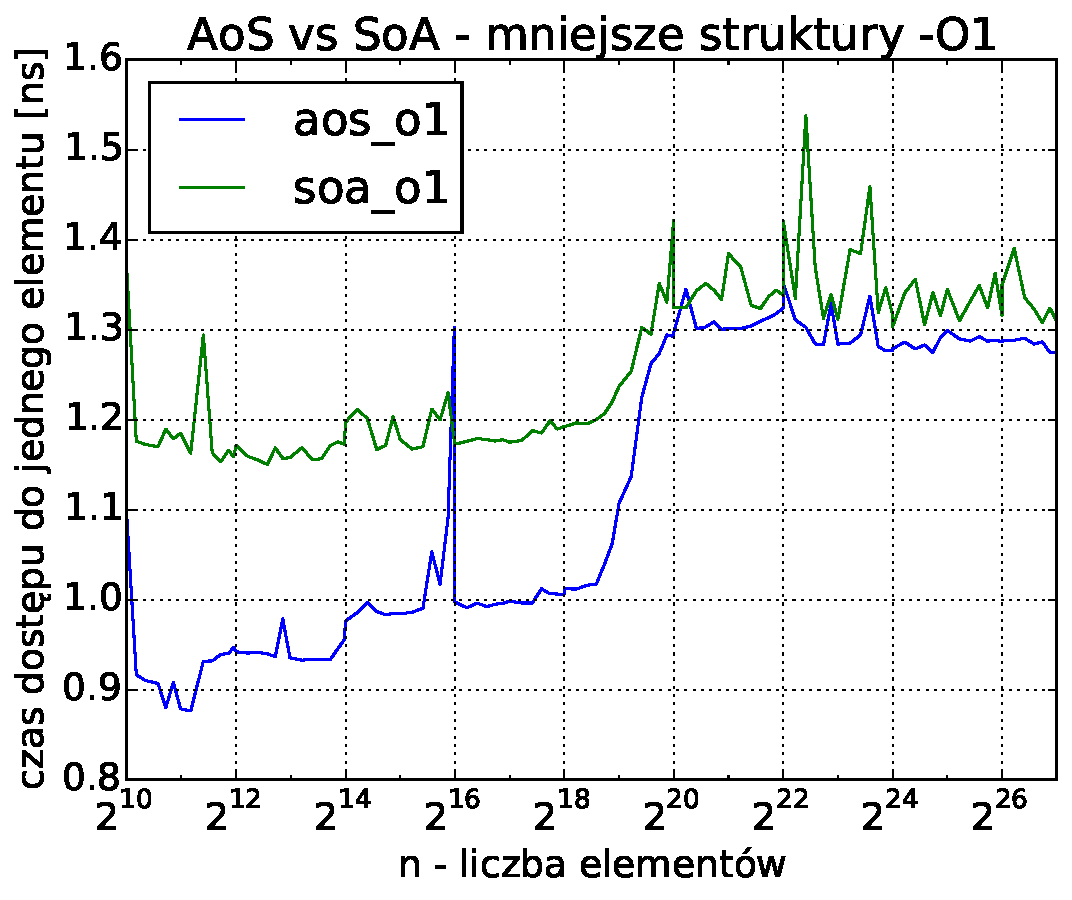
\includegraphics[width=\textwidth]{images/benchs_xeon/compact_aos_vs_soa_O1}
        \caption{Kompilacja z flagą \texttt{-O1}}
    \end{subfigure}
    \\
    \vspace{0.55cm}
    \begin{subfigure}[c]{0.45\textwidth}
        \centering
        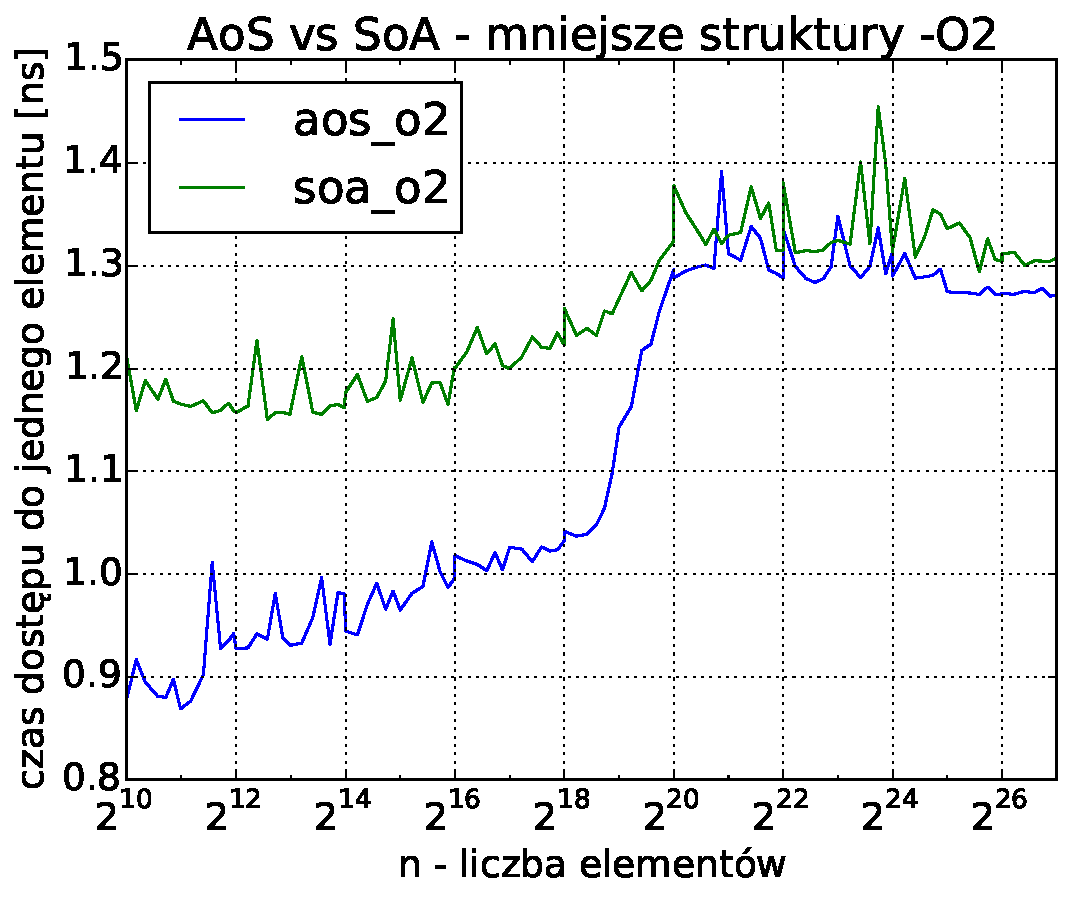
\includegraphics[width=\textwidth]{images/benchs_xeon/compact_aos_vs_soa_O2}
        \caption{Kompilacja z flagą \texttt{-O2}}
    \end{subfigure}
    ~
    \begin{subfigure}[c]{0.45\textwidth}
        \centering
        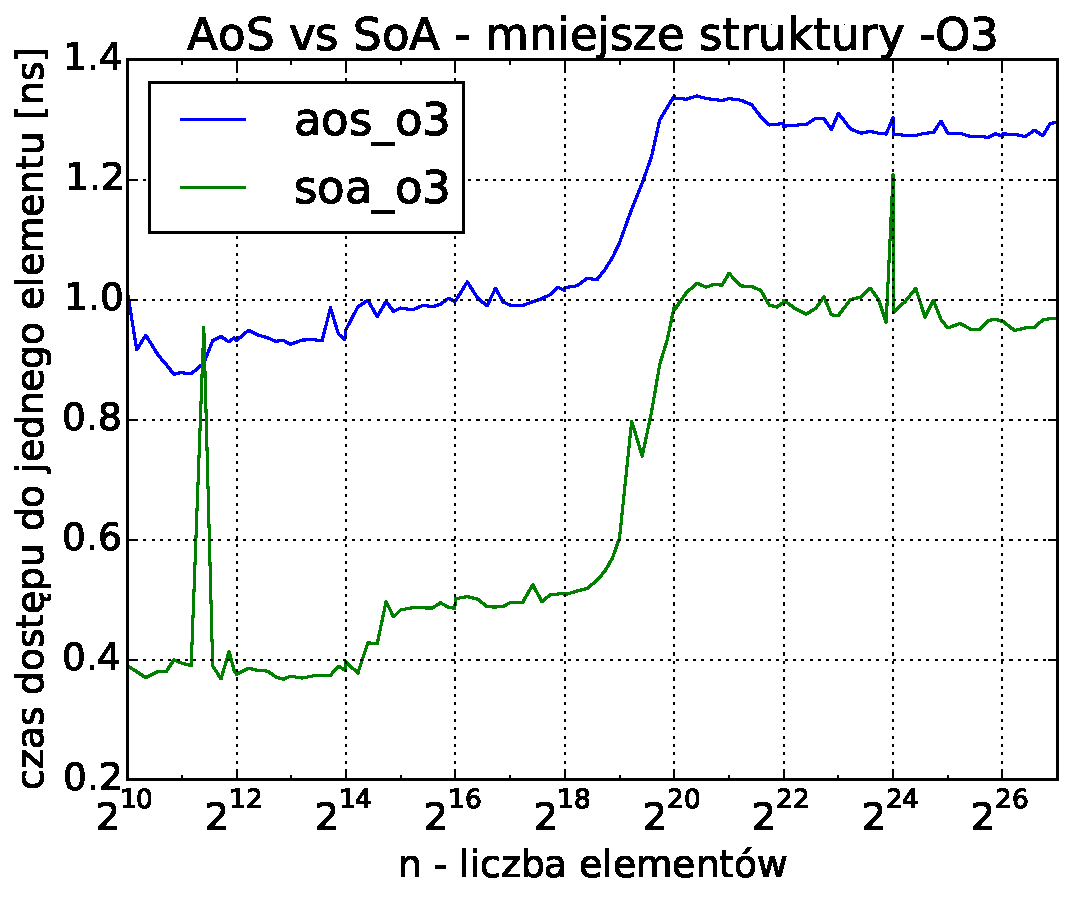
\includegraphics[width=\textwidth]{images/benchs_xeon/compact_aos_vs_soa_O3}
        \caption{Kompilacja z flagą \texttt{-O3}}
    \end{subfigure}
    \\
    \vspace{0.55cm}
    \begin{subfigure}[c]{1.0\textwidth}
        \centering
        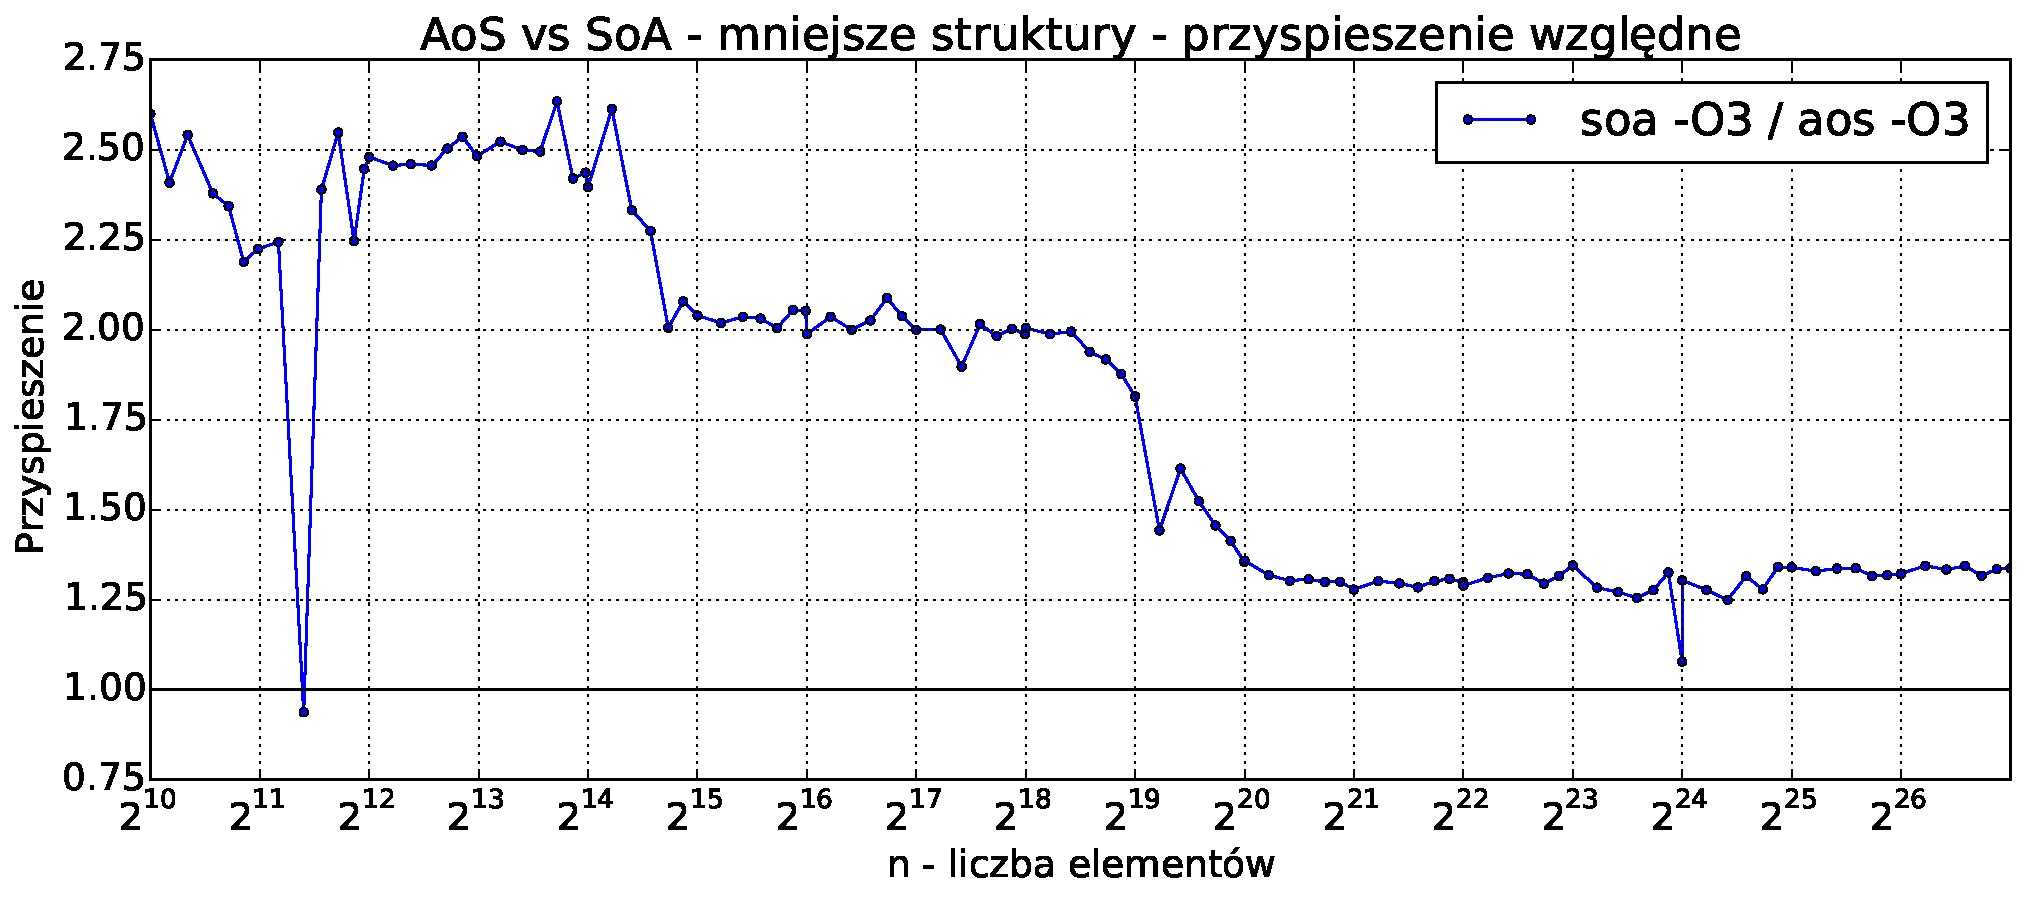
\includegraphics[width=0.80\textwidth]{images/benchs_xeon/compact_aos_vs_soa_normalized}
        \caption{Wydajność SoA względem AoS dla mniejszych struktur, dla flagi \texttt{-O3}.}
        \label{fig:compactAosVsSoaRelativeXeon}
    \end{subfigure}
    \caption{Wyniki testów AoS vs SoA dla mniejszych struktur (z sekcji \ref{sub:compactAosVsSoa}), dla~procesora Intel \mbox{Xeon W3565}.}
    \label{fig:compactAosLayoutXeon}
\end{figure}

\clearpage

\subsection{Dostęp swobodny}
\label{sub:randomAosVsSoa}

W poniższym przykładzie przeanalizowano swobodny dostęp do kompaktowych struktur danych AoS oraz SoA, przedstawionych wcześniej na~listingach \ref{lst:compactAos} oraz \ref{lst:compactSoa}. W~tym celu zmieniono algorytm sumowania elementów -- przedstawiono~go na~listingu \ref{lst:randomAosVsSoaImpl}.

\begin{lstlisting}[
    caption={Zmodyfikowany algorytm z listingów \ref{lst:aos} oraz \ref{lst:soa} -- dostęp odbywa się losowo, zamiast sekwencyjnie.},
    label=lst:randomAosVsSoaImpl
]
std::mt19937 gen;
std::uniform_int_distribution<> rnd(0, n - 1);
long int res = 0;
for (std::size_t i = 0; i < n; ++i) {
    auto idx = rnd(gen);
    // operacja sumowania zależna od podejścia - dla AoS:
    res += ps[idx].x + ps[idx].y + ps[idx].z;
    // lub w przypadku SoA:
    res += ps.x[idx] + ps.y[idx] + ps.z[idx];
}
return res;
\end{lstlisting}

Na rysunkach \ref{fig:randomAosVsSoa} oraz \ref{fig:randomAosVsSoaXeon} przedstawiono wyniki dla dwóch różnych procesorów. Jak można zauważyć, w przypadku swobodnego dostępu dla dużej liczby elementów, lepiej wykorzystać ,,standardowe'' podejście obiektowe, czyli tablicę struktur (AoS), ponieważ dla SoA traci się około 20\% wydajności, co~widać na~wykresach~\ref{fig:randomAosVsSoaRelative} oraz \ref{fig:randomAosVsSoaRelativeXeon}.

W przypadku gdy dane wciąż mieszczą się w pamięci podręcznej, a dostęp do danych jest powtarzalny, wydajność jest na zbliżonym poziomie.

\begin{figure}[!h]
    \centering
    \begin{subfigure}[c]{0.45\textwidth}
        \centering
        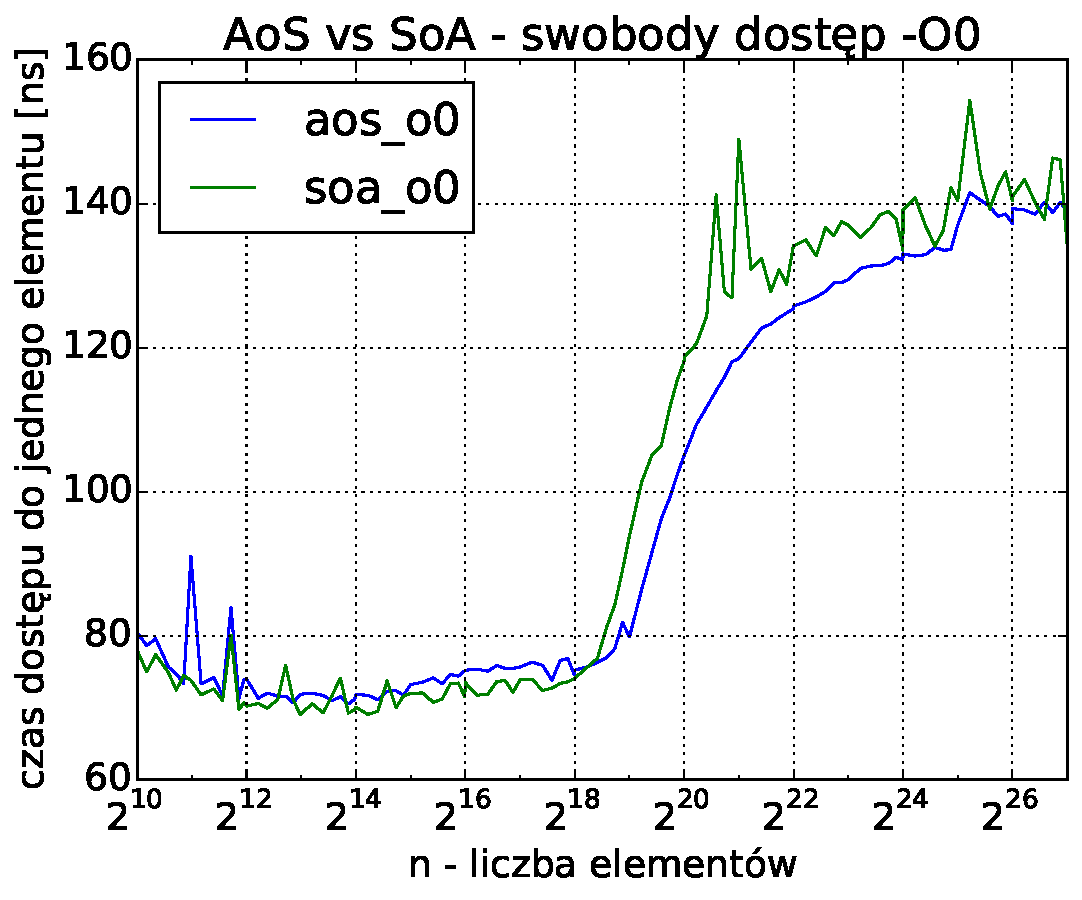
\includegraphics[width=\textwidth]{images/benchs/random_access_aos_vs_soa_O0}
        \caption{Kompilacja z flagą \texttt{-O0}}
    \end{subfigure}
    ~
    \begin{subfigure}[c]{0.45\textwidth}
        \centering
        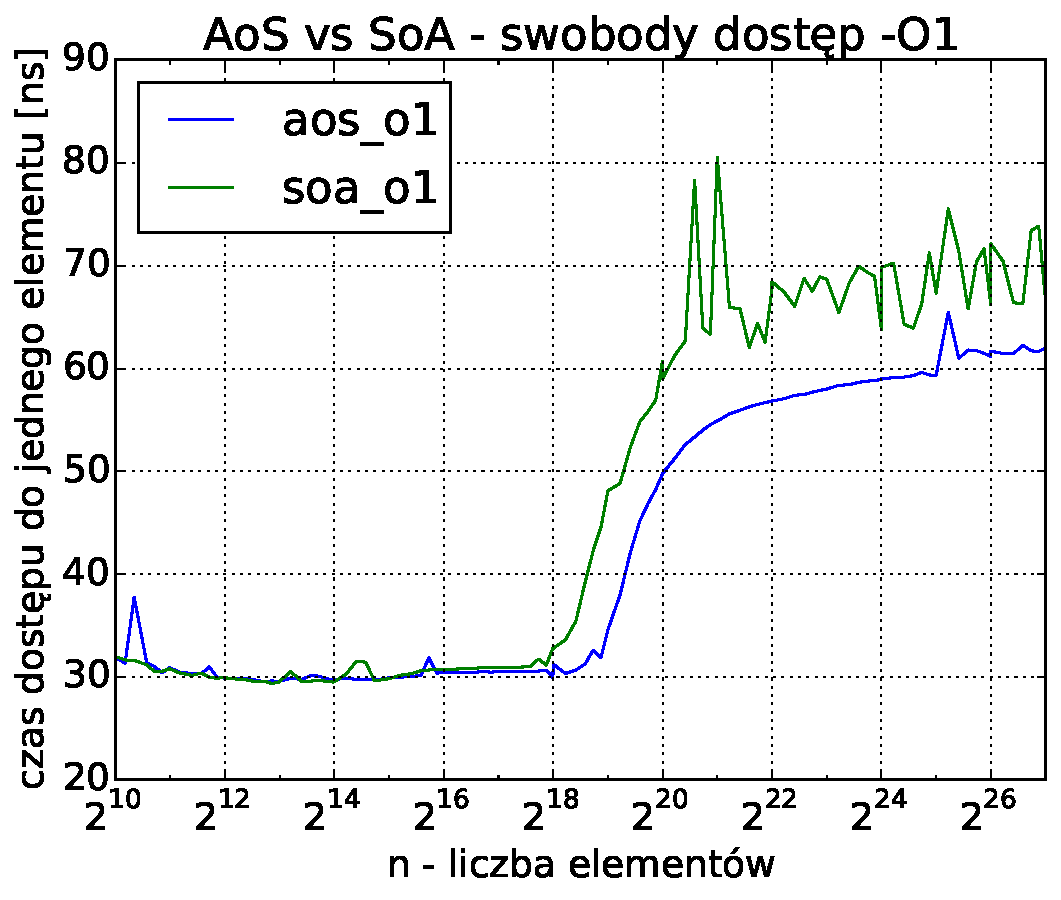
\includegraphics[width=\textwidth]{images/benchs/random_access_aos_vs_soa_O1}
        \caption{Kompilacja z flagą \texttt{-O1}}
    \end{subfigure}
    \\
    \vspace{0.55cm}
    \begin{subfigure}[c]{0.45\textwidth}
        \centering
        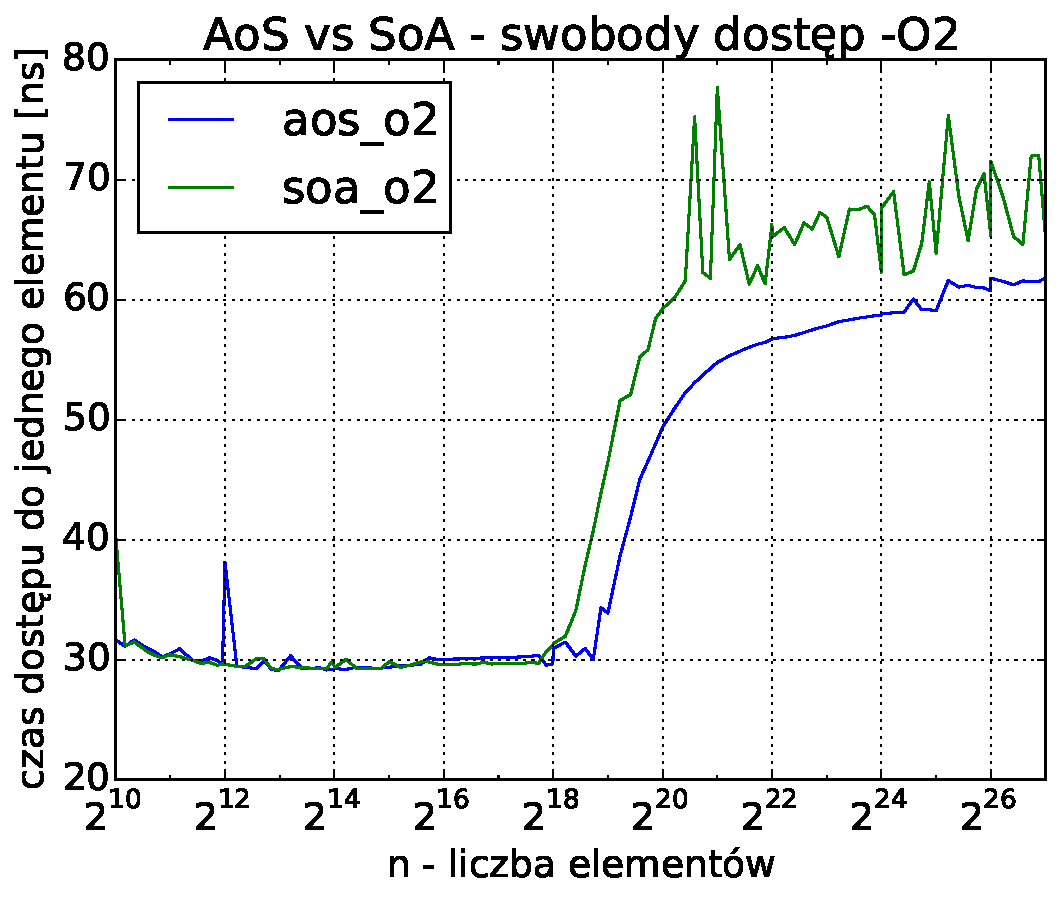
\includegraphics[width=\textwidth]{images/benchs/random_access_aos_vs_soa_O2}
        \caption{Kompilacja z flagą \texttt{-O2}}
    \end{subfigure}
    ~
    \begin{subfigure}[c]{0.45\textwidth}
        \centering
        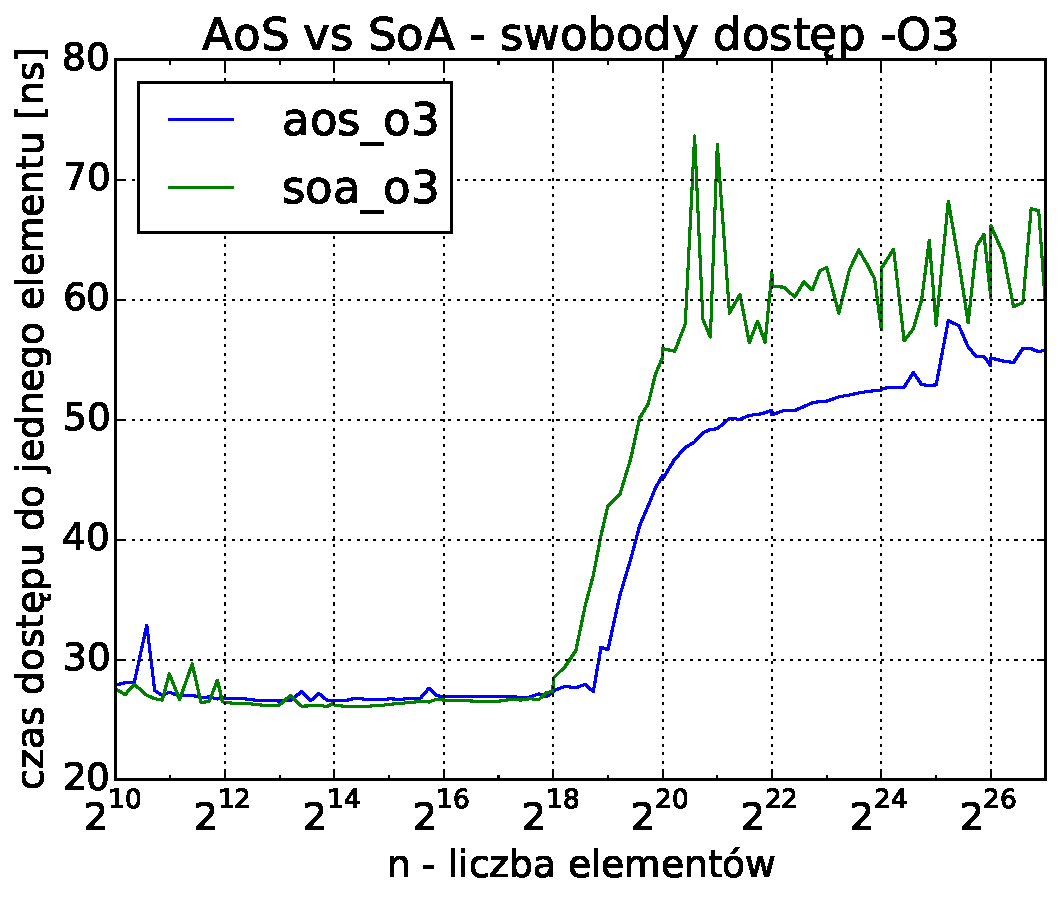
\includegraphics[width=\textwidth]{images/benchs/random_access_aos_vs_soa_O3}
        \caption{Kompilacja z flagą \texttt{-O3}}
    \end{subfigure}
    \\
    \vspace{0.55cm}
    \begin{subfigure}[c]{1.0\textwidth}
        \centering
        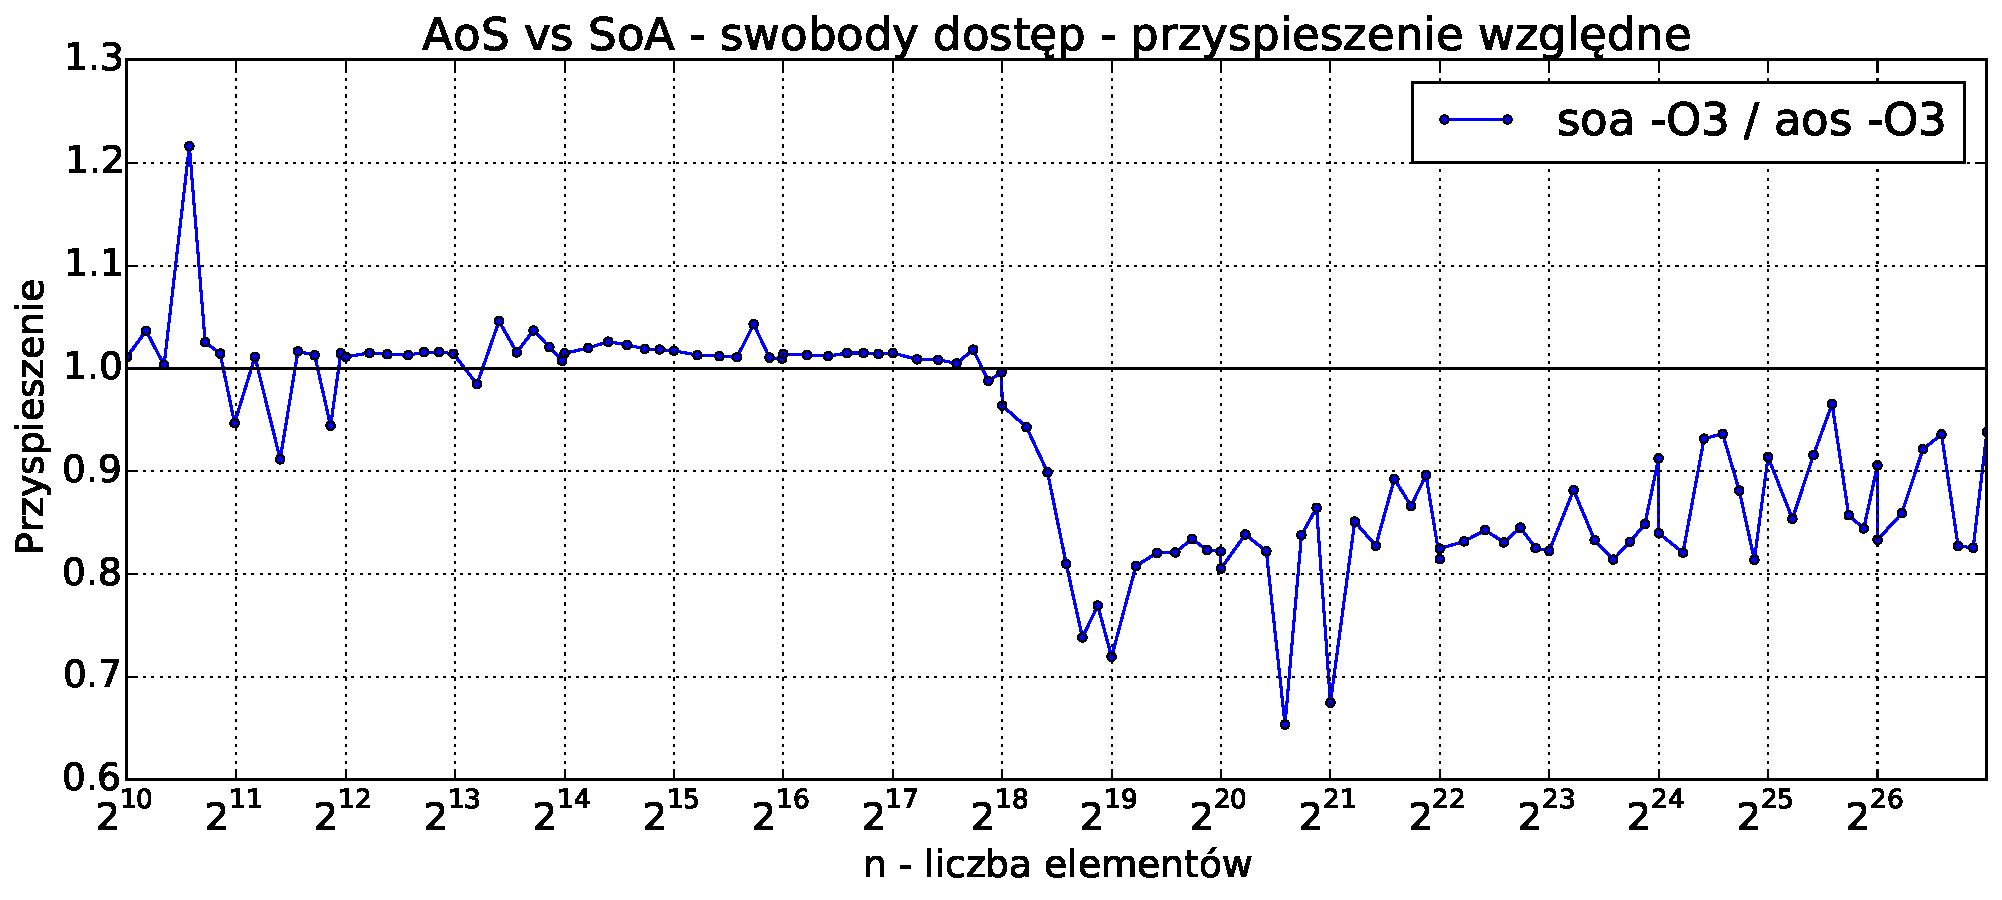
\includegraphics[width=0.80\textwidth]{images/benchs/random_access_aos_vs_soa_normalized}
        \caption{Wydajność SoA względem AoS dla swobodnego dostępu, dla flagi \texttt{-O3}.}
        \label{fig:randomAosVsSoaRelative}
    \end{subfigure}
    \caption{Wyniki testów AoS vs SoA dla swobodnego dostępu (z sekcji \ref{sub:randomAosVsSoa}), dla~procesora \mbox{Intel i7-4720HQ}.}
    \label{fig:randomAosVsSoa}
\end{figure}

\clearpage

\begin{figure}[!h]
    \centering
    \begin{subfigure}[c]{0.45\textwidth}
        \centering
        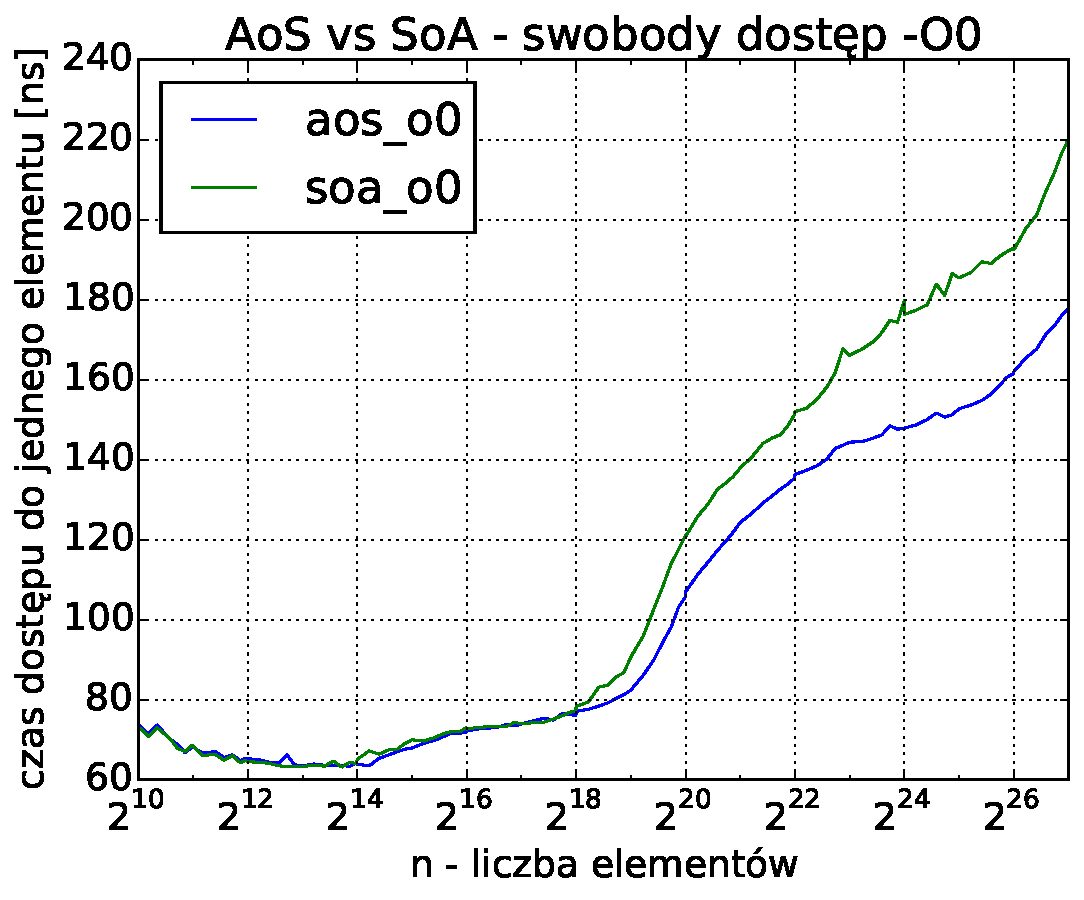
\includegraphics[width=\textwidth]{images/benchs_xeon/random_access_aos_vs_soa_O0}
        \caption{Kompilacja z flagą \texttt{-O0}}
    \end{subfigure}
    ~
    \begin{subfigure}[c]{0.45\textwidth}
        \centering
        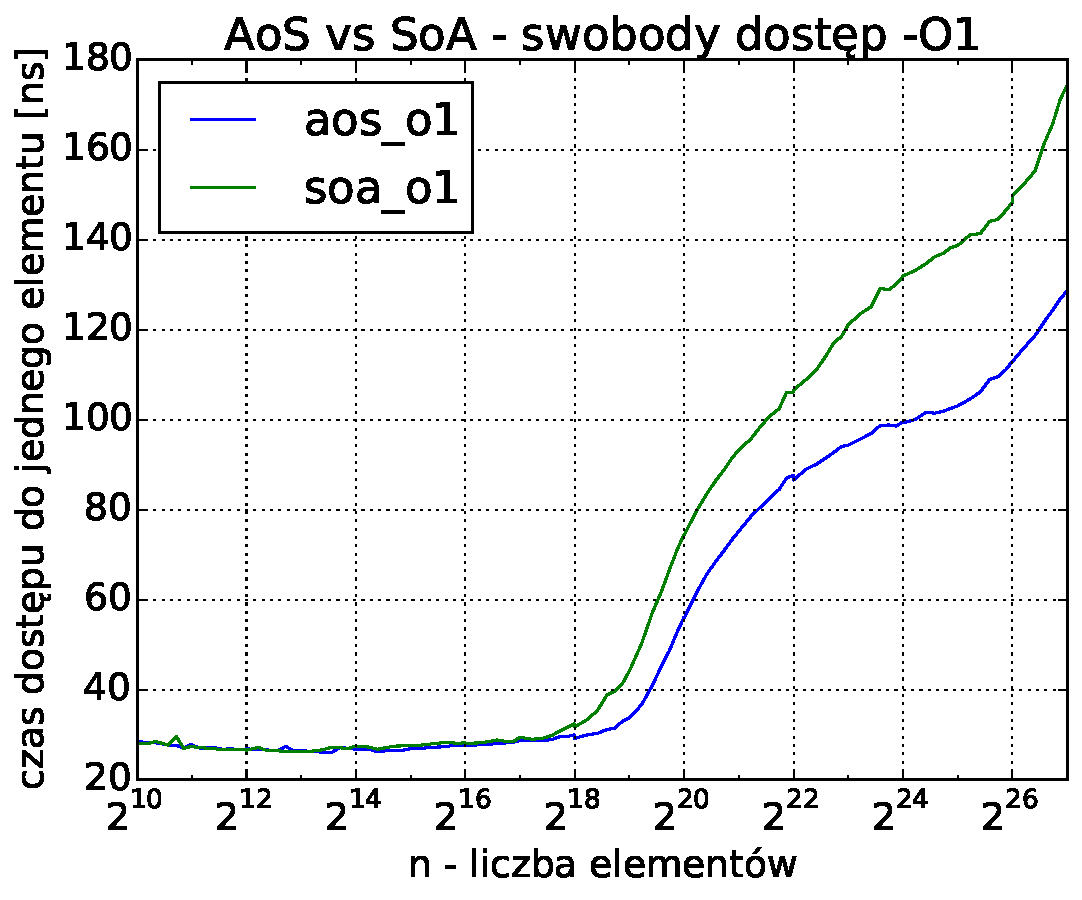
\includegraphics[width=\textwidth]{images/benchs_xeon/random_access_aos_vs_soa_O1}
        \caption{Kompilacja z flagą \texttt{-O1}}
    \end{subfigure}
    \\
    \vspace{0.55cm}
    \begin{subfigure}[c]{0.45\textwidth}
        \centering
        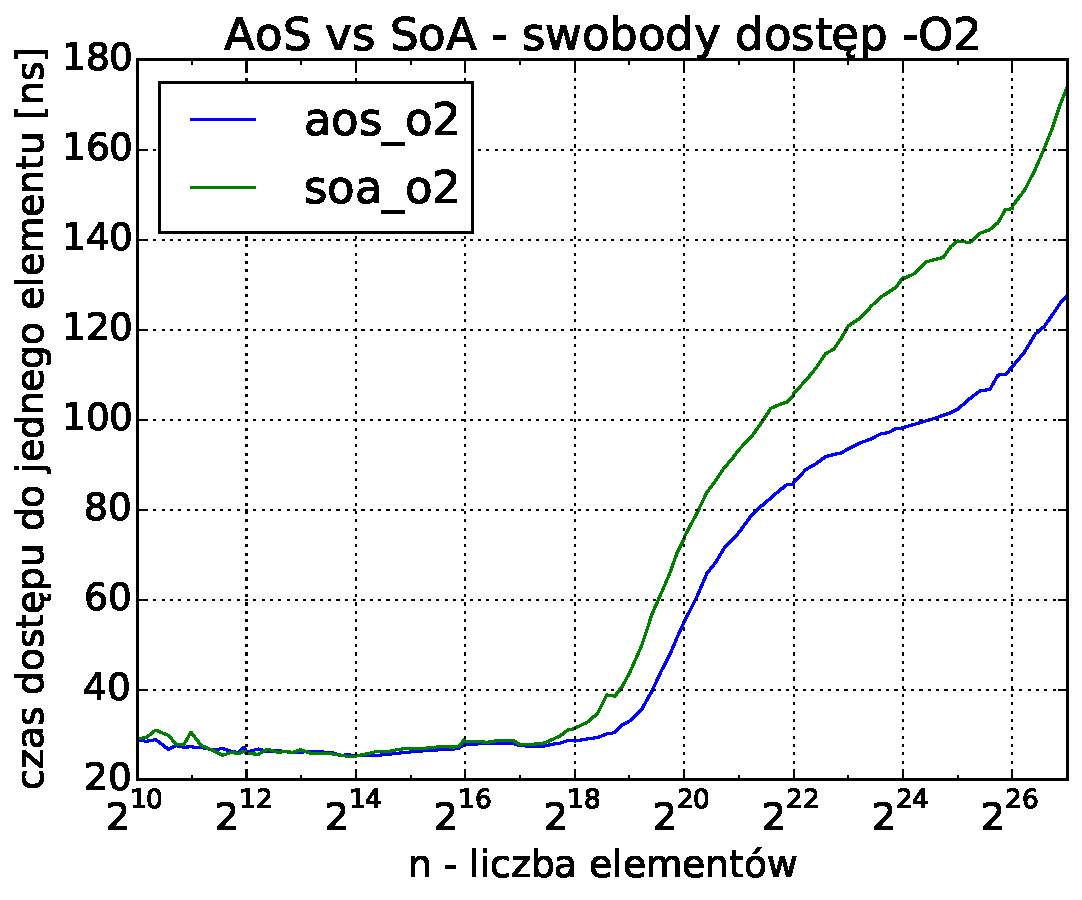
\includegraphics[width=\textwidth]{images/benchs_xeon/random_access_aos_vs_soa_O2}
        \caption{Kompilacja z flagą \texttt{-O2}}
    \end{subfigure}
    ~
    \begin{subfigure}[c]{0.45\textwidth}
        \centering
        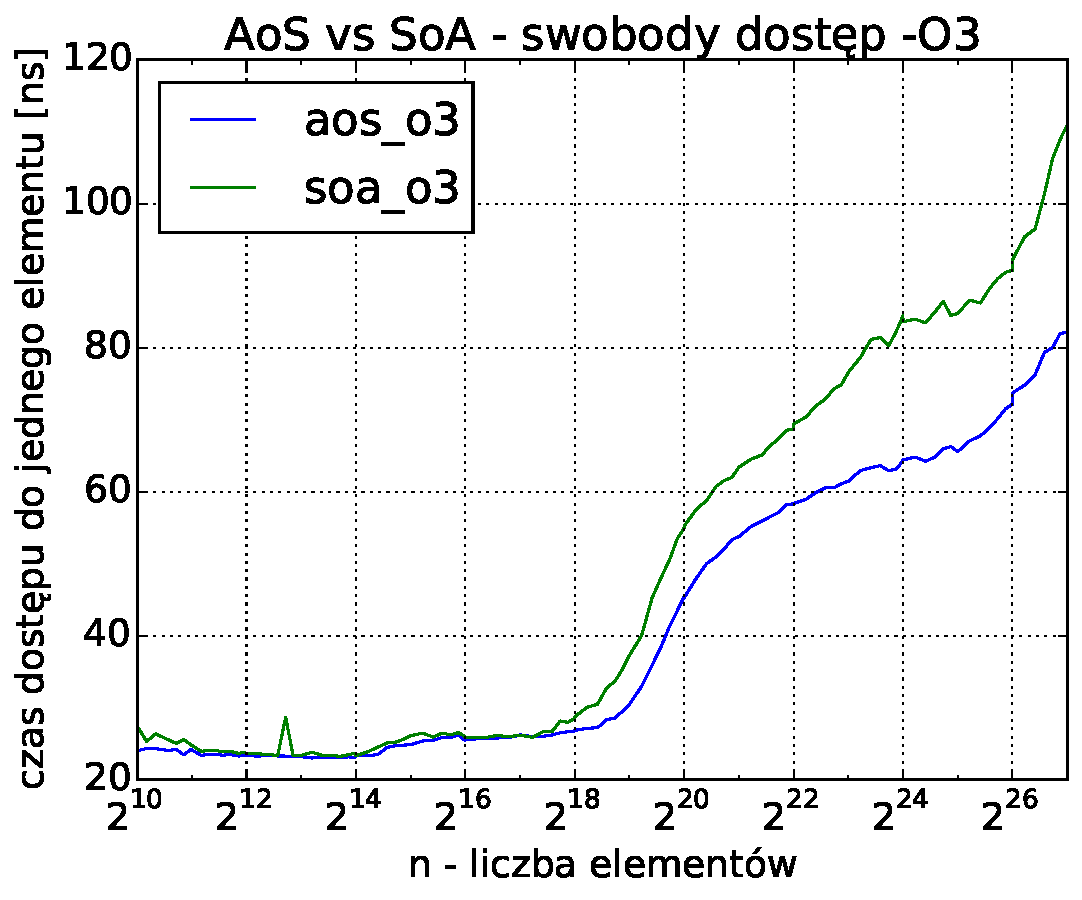
\includegraphics[width=\textwidth]{images/benchs_xeon/random_access_aos_vs_soa_O3}
        \caption{Kompilacja z flagą \texttt{-O3}}
    \end{subfigure}
    \\
    \vspace{0.55cm}
    \begin{subfigure}[c]{1.0\textwidth}
        \centering
        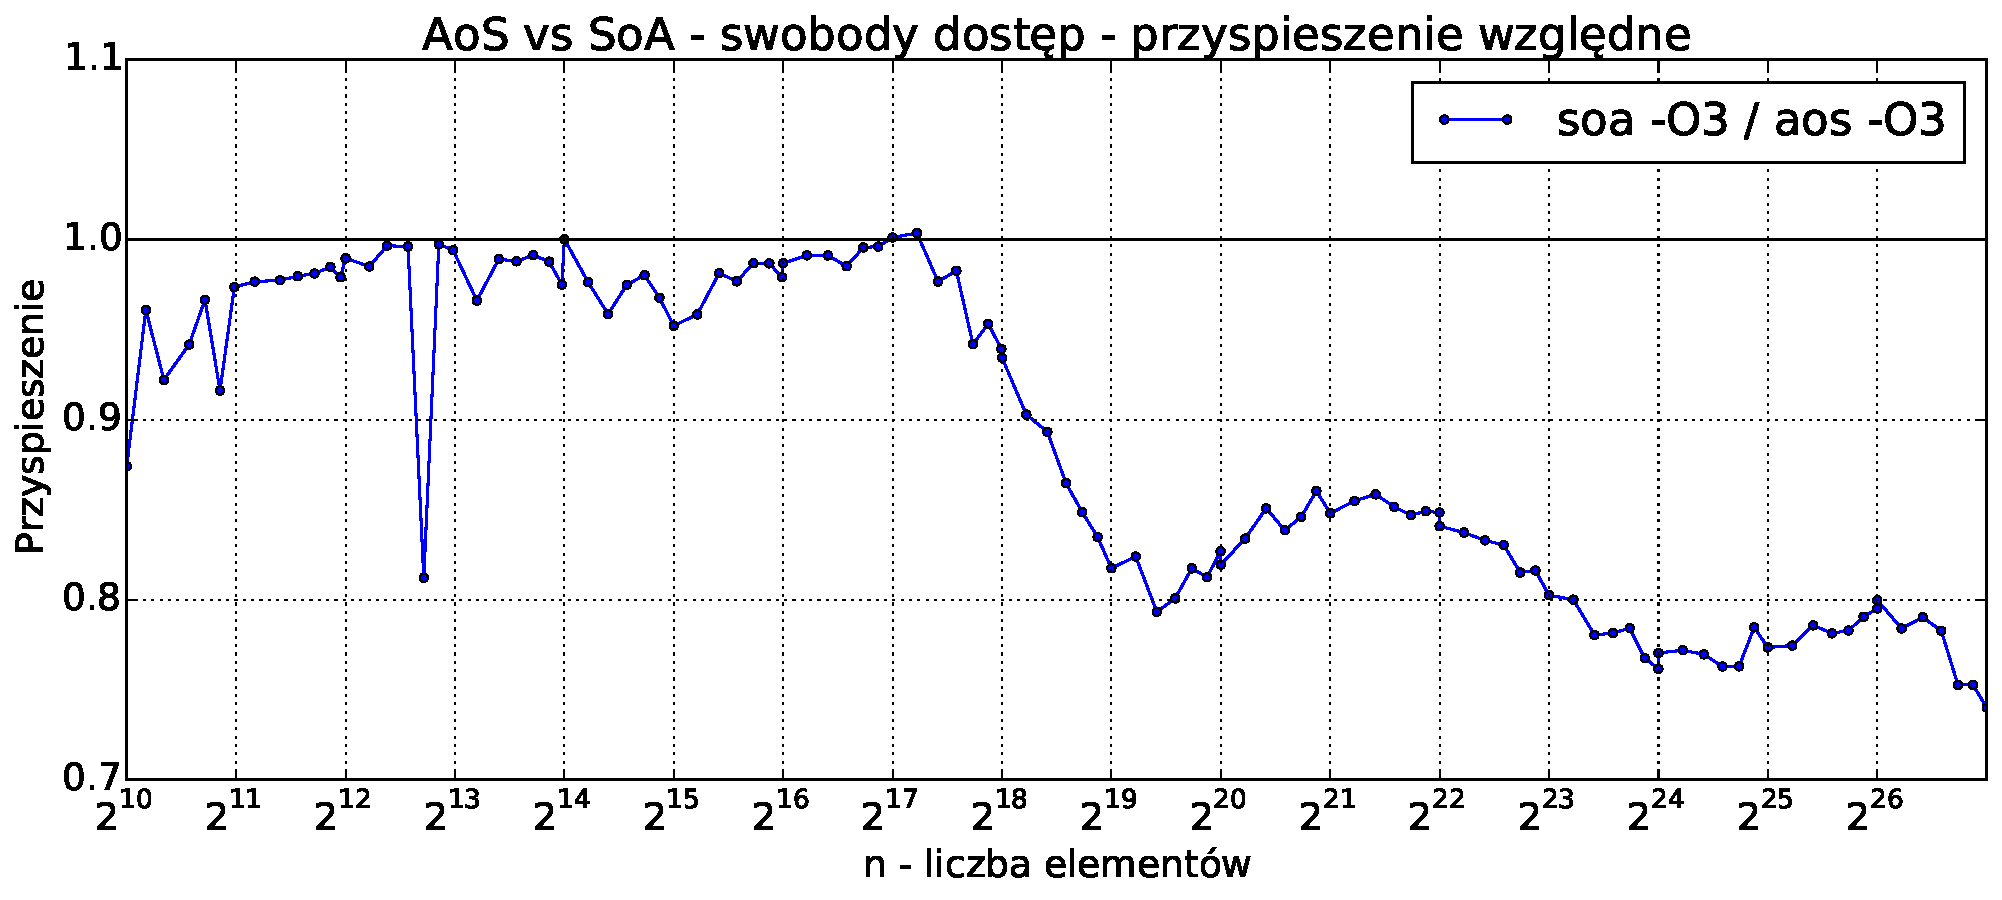
\includegraphics[width=0.80\textwidth]{images/benchs_xeon/random_access_aos_vs_soa_normalized}
        \caption{Wydajność SoA względem AoS dla swobodnego dostępu, dla flagi \texttt{-O3}.}
        \label{fig:randomAosVsSoaRelativeXeon}
    \end{subfigure}
    \caption{Wyniki testów AoS vs SoA dla swobodnego dostępu (z sekcji \ref{sub:randomAosVsSoa}), dla~procesora \mbox{Intel Xeon W3565}.}
    \label{fig:randomAosVsSoaXeon}
\end{figure}

\clearpage % TODO/FIXME

\section{Przetwarzanie warunkowe}
\label{sub:filteredSum}

Przetwarzanie warunkowe polega na~przetworzeniu danych, bazując na określonym warunku. Dla~tego zagadnienia zbadano problem polegający na sumowaniu elementów wektora, które są większe lub równe 128 \cite{MindTheCache_FilteredSum}. Wektor został wypełniony losowymi elementami od 0 do 255\footnote{W obu przypadkach tymi samymi, ponieważ ziarno generatora liczb pseudolosowych pomiędzy wywołaniami programu jest takie samo.}. Porównano dwa podejścia -- gdy wektor jest nieposortowany oraz gdy został posortowany. Samo sortowanie nie zostało wliczone w czas wykonania. Testowana funkcja to lambda \texttt{f} z linii 11-17 listingu \ref{lst:filteredSum}.

\begin{lstlisting}[float=!ht, caption={Kod sumowania elementów większych niż 128.}, label=lst:filteredSum,
numbers=left,
stepnumber=1,    
firstnumber=1,
numberfirstline=true]
std::vector<int> v;

// wypełnienie wektora losowymi elementami z zakresu [0, 255]
std::mt19937 gen;
std::uniform_int_distribution<> rnd(0, 255);
v.reserve(n); // n - liczba elementów w wektorze
for (std::size_t i = 0; i < n; ++i)
    v.push_back(rnd(gen));

// mierzona funkcja
auto f = [&]() {
    long int res = 0;
    for (int x: v)
        if (x >= 128)
            res += x;
    return res;
};
\end{lstlisting}

Na~rysunkach \ref{fig:filteredSum} oraz \ref{fig:filteredSumXeon} zostały zaprezentowane wyniki testów wydajności dla dwóch omówionych procesorów, a~w~tabeli \ref{tab:FilteredSumPerf} statystyki uzyskane programem perf dla wybranego rozmiaru wektora dla kompilacji z~flagą optymalizacji \texttt{-O2} dla procesora Intel i7 4720hq (przyczyna wybrania flagi jest~opisana poniżej). 

\begin{figure}
    \centering
    \begin{subfigure}[c]{0.45\textwidth}
        \centering
        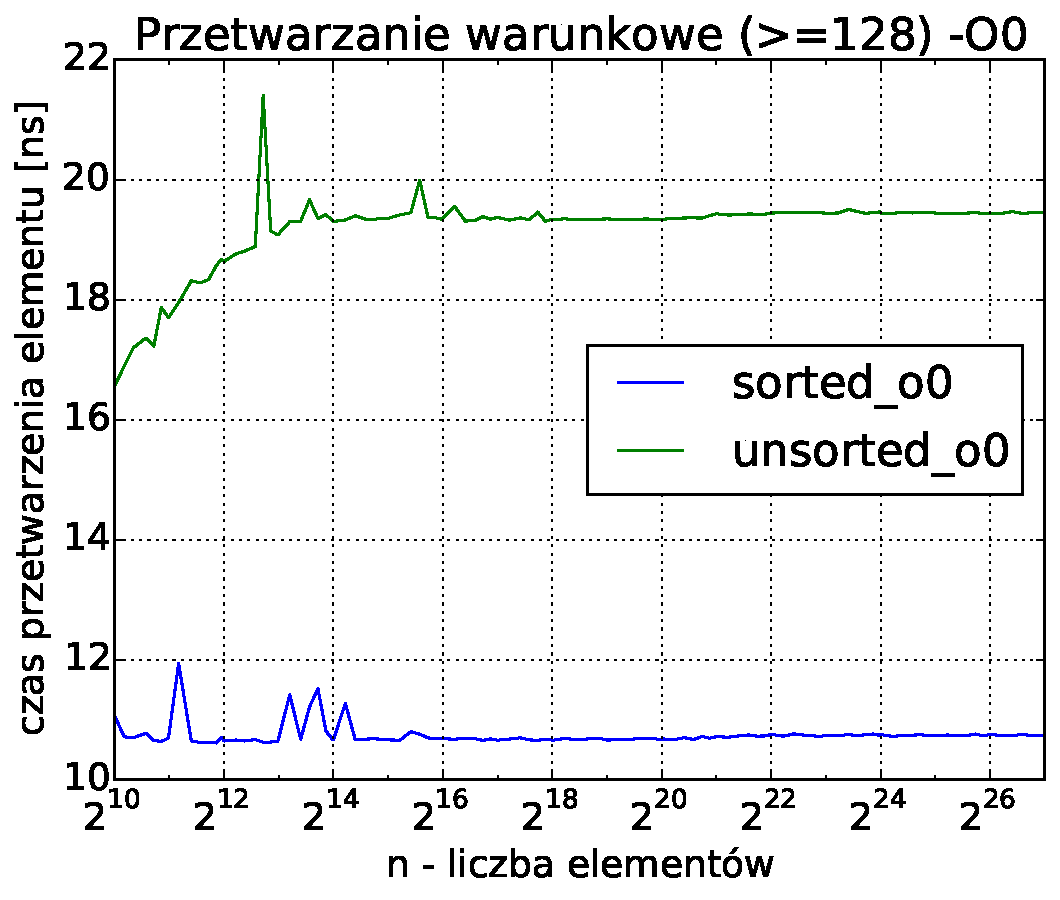
\includegraphics[width=\textwidth]{images/benchs/filtered_sum_O0}
        \caption{Kompilacja z flagą \texttt{-O0}}
    \end{subfigure}
    ~
    \begin{subfigure}[c]{0.45\textwidth}
        \centering
        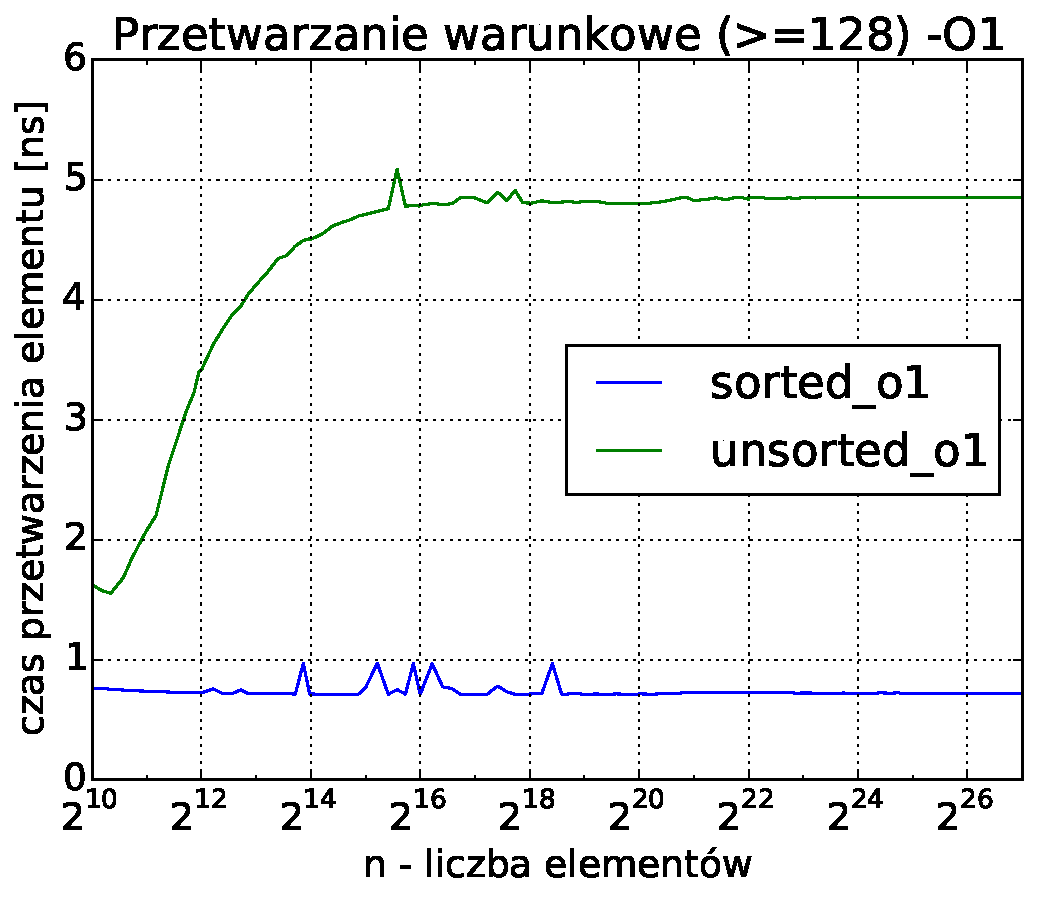
\includegraphics[width=\textwidth]{images/benchs/filtered_sum_O1}
        \caption{Kompilacja z flagą \texttt{-O1}}
    \end{subfigure}
    \\
    \vspace{0.55cm}
    \begin{subfigure}[c]{0.45\textwidth}
        \centering
        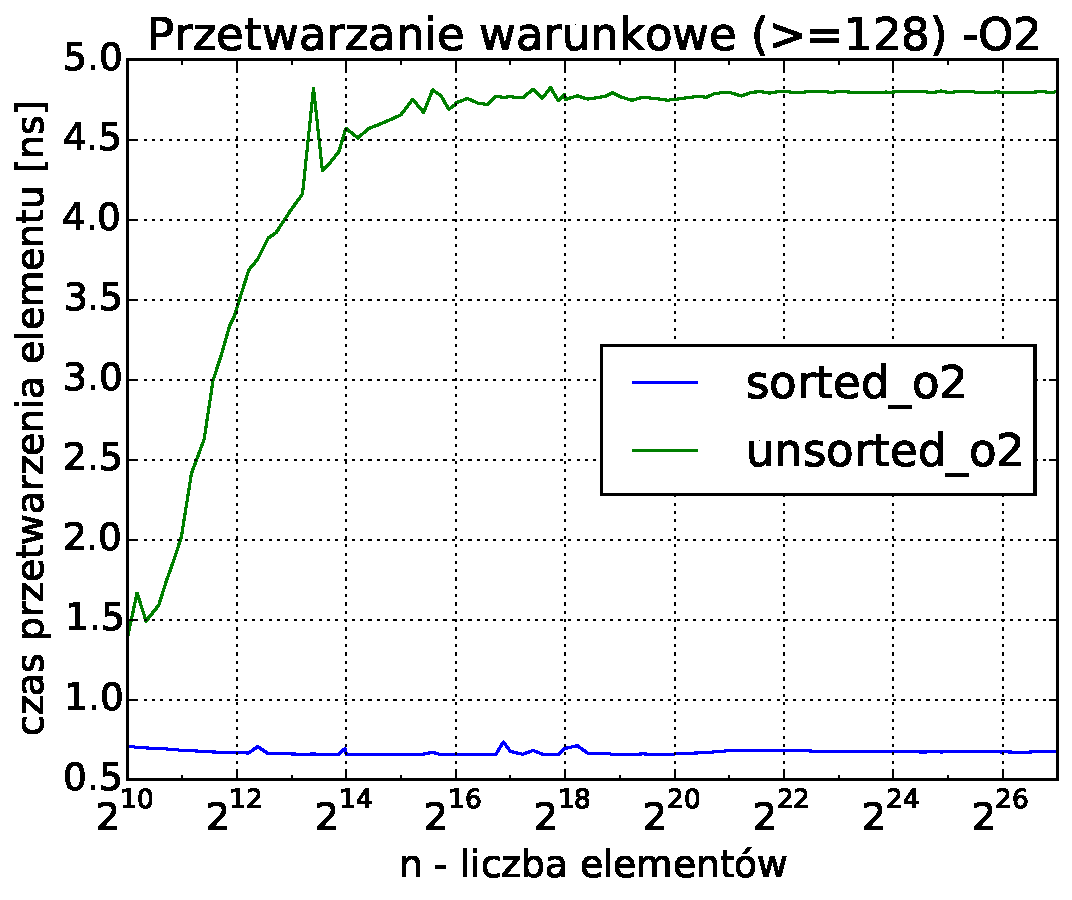
\includegraphics[width=\textwidth]{images/benchs/filtered_sum_O2}
        \caption{Kompilacja z flagą \texttt{-O2}}
    \end{subfigure}
    ~
    \begin{subfigure}[c]{0.45\textwidth}
        \centering
        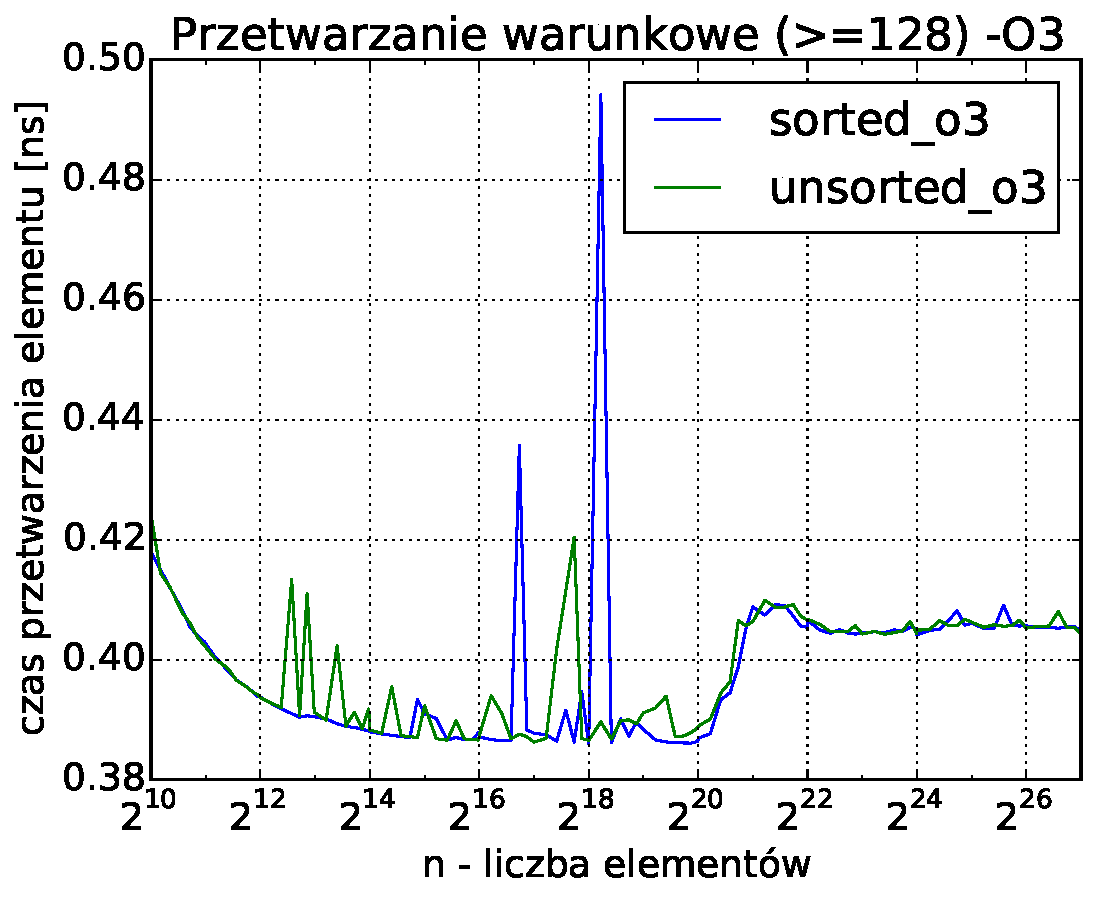
\includegraphics[width=\textwidth]{images/benchs/filtered_sum_O3}
        \caption{Kompilacja z flagą \texttt{-O3}}
    \end{subfigure}
    \\
    \vspace{0.55cm}
    \begin{subfigure}[c]{1.0\textwidth}
        \centering
        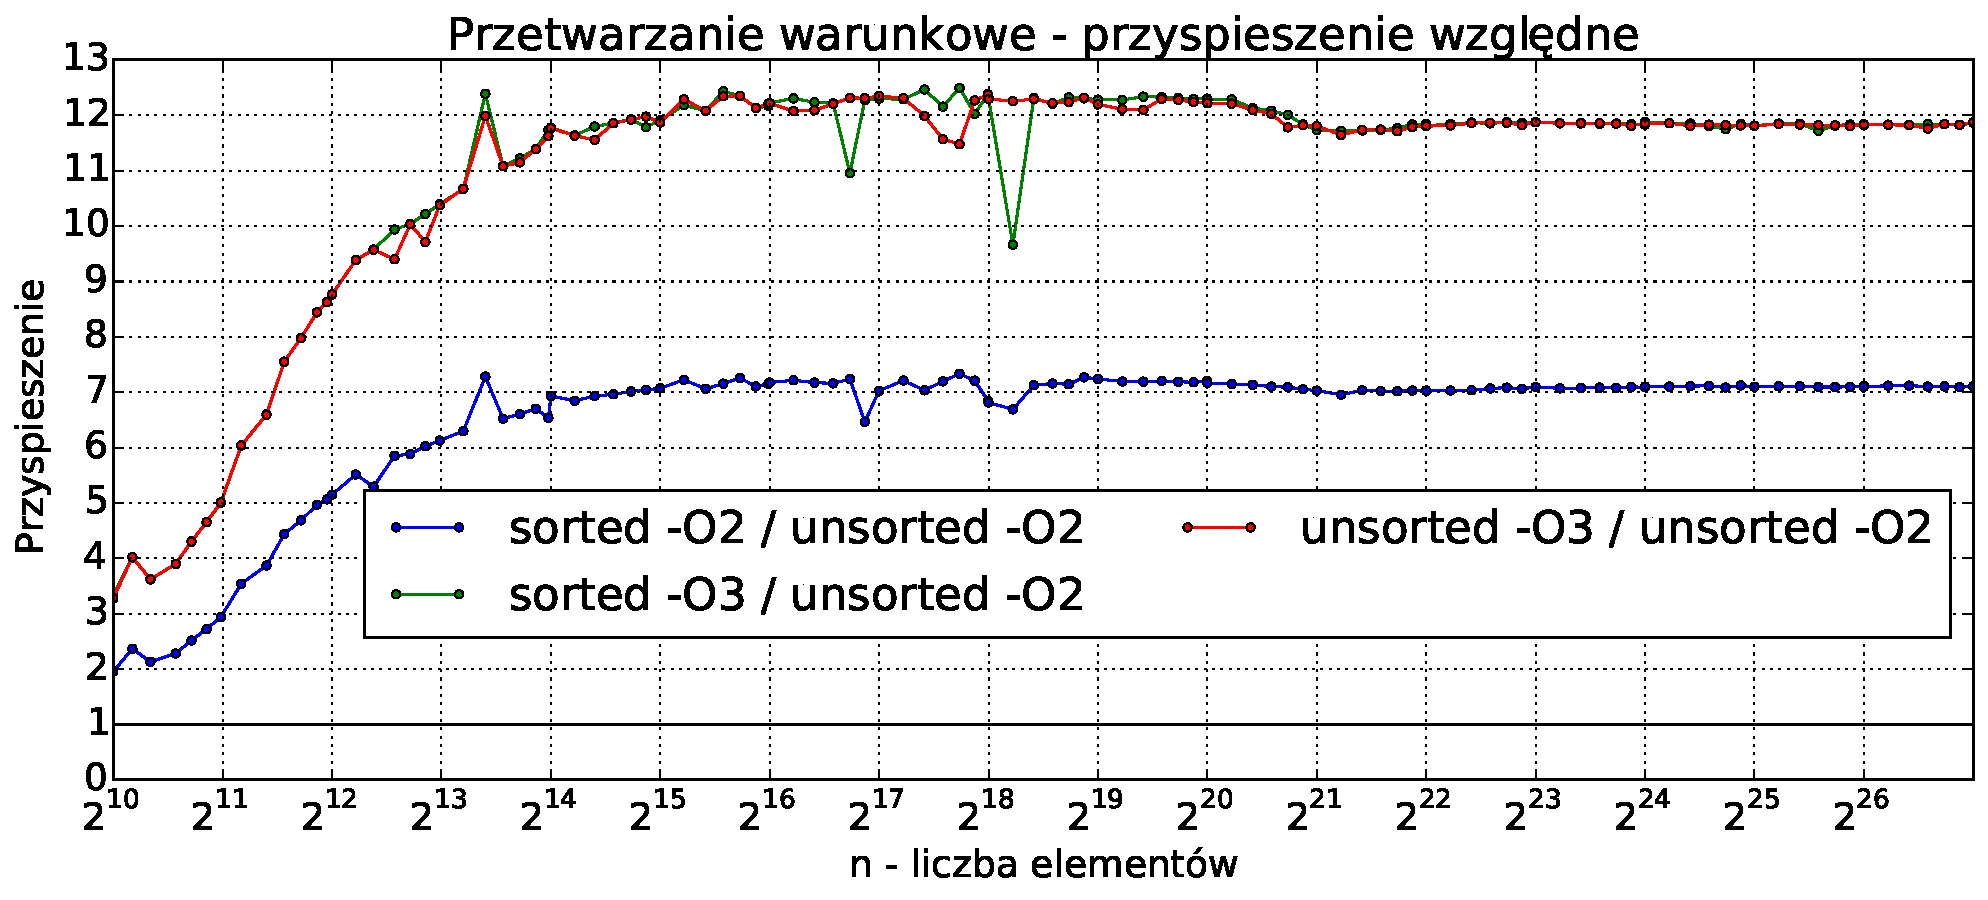
\includegraphics[width=0.80\textwidth]{images/benchs/filtered_sum_normalized}
        \caption{Przyspieszenie uzyskane względem przypadku nieposortowanych danych przy kompilacji z flagą \texttt{-O2}.}
        \label{fig:filteredSumRelative}
    \end{subfigure}
    \caption{Wyniki testów przetwarzania warunkowego (z sekcji \ref{sub:filteredSum}), dla~procesora Intel i7-4720HQ.}
    \label{fig:filteredSum}
\end{figure}

\clearpage

\begin{figure}[!h]
    \centering
    \begin{subfigure}[c]{0.45\textwidth}
        \centering
        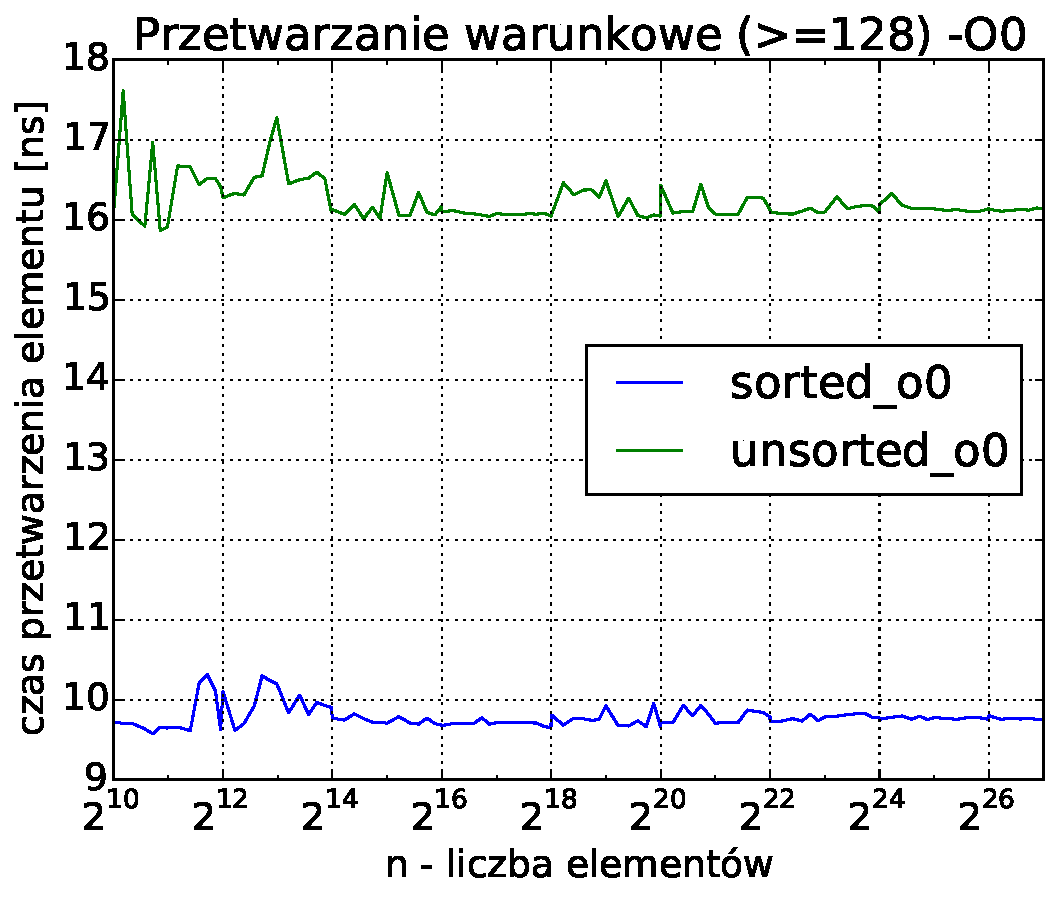
\includegraphics[width=\textwidth]{images/benchs_xeon/filtered_sum_O0}
        \caption{Kompilacja z flagą \texttt{-O0}}
    \end{subfigure}
    ~
    \begin{subfigure}[c]{0.45\textwidth}
        \centering
        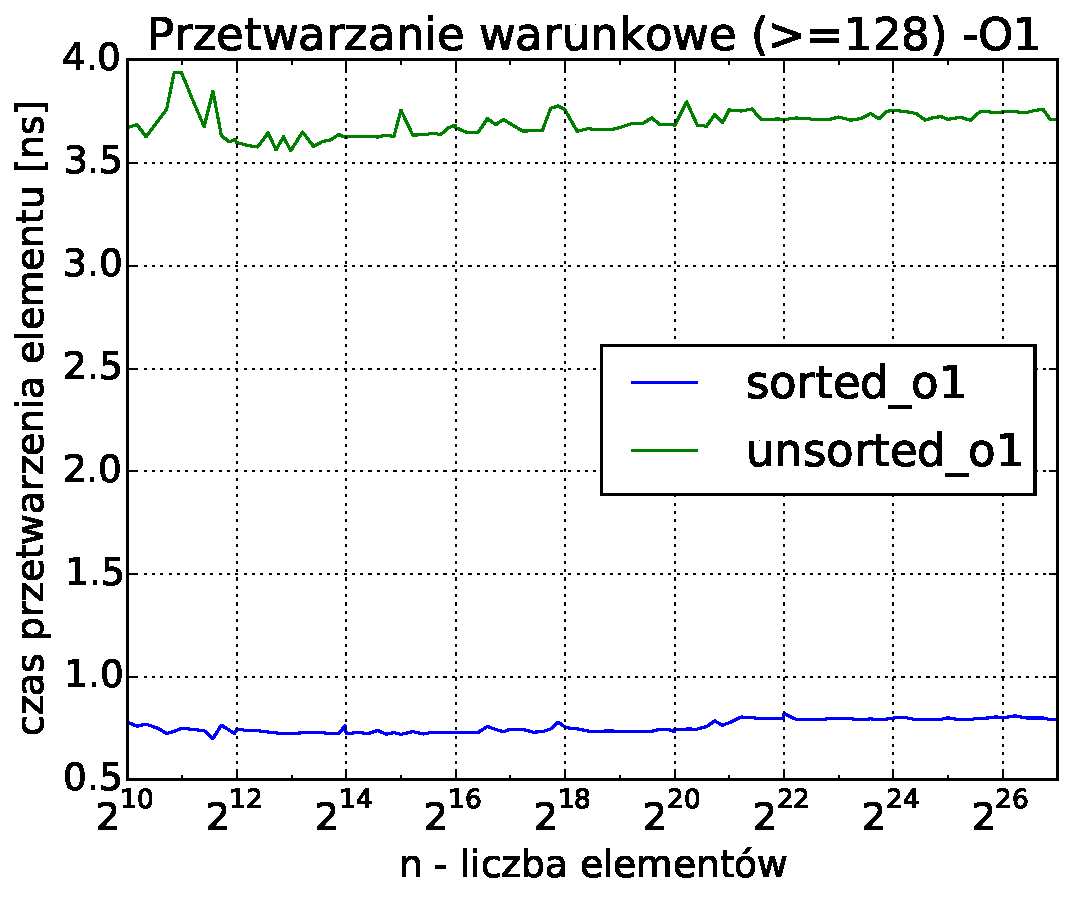
\includegraphics[width=\textwidth]{images/benchs_xeon/filtered_sum_O1}
        \caption{Kompilacja z flagą \texttt{-O1}}
    \end{subfigure}
    \\
    \vspace{0.55cm}
    \begin{subfigure}[c]{0.45\textwidth}
        \centering
        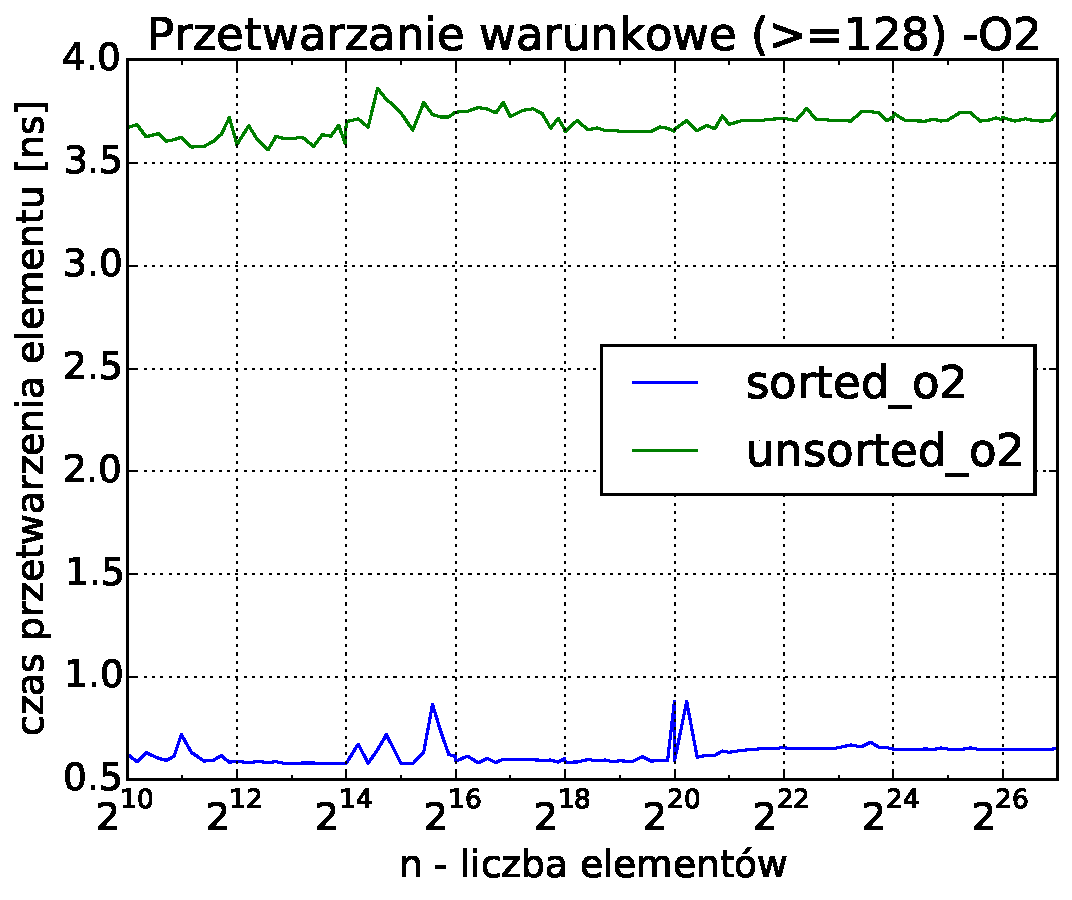
\includegraphics[width=\textwidth]{images/benchs_xeon/filtered_sum_O2}
        \caption{Kompilacja z flagą \texttt{-O2}}
    \end{subfigure}
    ~
    \begin{subfigure}[c]{0.45\textwidth}
        \centering
        \includegraphics[width=\textwidth]{images/benchs_xeon/filtered_sum_O3}
        \caption{Kompilacja z flagą \texttt{-O3}}
    \end{subfigure}
    \\
    \vspace{0.55cm}
    \begin{subfigure}[c]{1.0\textwidth}
        \centering
        \includegraphics[width=0.80\textwidth]{images/benchs_xeon/filtered_sum_normalized}
        \caption{Przyspieszenie uzyskane względem przypadku nieposortowanych danych przy kompilacji z flagą \texttt{-O2}.}
        \label{fig:filteredSumRelativeXeon}
    \end{subfigure}
    \caption{Wyniki testów przetwarzania warunkowego (z sekcji \ref{sub:filteredSum}), dla~procesora Intel \mbox{Xeon W3565}.}
    \label{fig:filteredSumXeon}
\end{figure}


\begin{table}
    \centering
    \caption{Statystyki programu perf dla problemu z sekcji \ref{sub:filteredSum} w wersji z optymalizacją \texttt{-O2}. W~kolejnych komórkach znajdują się uśrednione statystyki z~20 przebiegów programu dla wybranych rozmiarów wektora. Szare wiersze oznaczają posortowane dane.\\
    \textbf{1} -- liczba elementów wektora.\\
    \textbf{2} -- średni czas dostępu do jednego elementu [ns].\\
    \textbf{3} -- liczba wykonanych instrukcji.\\
    \textbf{4} -- liczba chybionych gałęzi (ang. \textit{branch misses}) [\%].\\
    \textbf{5} -- liczba chybień do cache L1d (danych) [\%].\\
    \textbf{6} -- liczba chybień do cache L3 [\%].\\}
    \label{tab:FilteredSumPerf}
    \begin{tabular}{
            |l|S[table-format=1.2]|S[table-format=11.0]|S[table-format=2.2]|S[table-format=1.2]|S[table-format=2.2]|
    }
        \hline
        \multicolumn{1}{|c}{\textbf{1}} & 
        \multicolumn{1}{|c}{\textbf{2}} & 
        \multicolumn{1}{|c}{\textbf{3}} & 
        \multicolumn{1}{|c}{\textbf{4}} & 
        \multicolumn{1}{|c}{\textbf{5}} & 
        \multicolumn{1}{|c|}{\textbf{6}}
        \\ \hline \hline
        \rowcolor{lgray} $2^{18}$ & 0.61 & 178052185 & 2.93 & 6.19 & 3.64
        \\ \hline
        $2^{18}$  & 3.63 & 124947938 & 20.44 & 6.21 & 16.23
        \\ \hline
        \rowcolor{lgray} $2^{19}$ & 0.51 & 244598497 & 1.67 & 1.7 & 1.98
        \\ \hline
        $2^{19}$  & 3.71 & 192833009 & 22.22 & 5.24 & 15.66
        \\ \hline
        \rowcolor{lgray} $2^{20}$ & 0.5 & 589022167 & 2.81 & 3.07 & 22.91
        \\ \hline
        $2^{20}$  & 3.65 & 434235010 & 22.48 & 4.78 & 62.49
        \\ \hline
        \rowcolor{lgray} $2^{21}$ & 0.53 & 1237576961 & 2.24 & 3.64 & 46.43
        \\ \hline
        $2^{21}$  & 3.65 & 870883135 & 21.98 & 5.43 & 74.07
        \\ \hline
        \rowcolor{lgray} $2^{22}$ & 0.52 & 2448258888 & 2.6 & 4.29 & 38.15
        \\ \hline
        $2^{22}$  & 3.62 & 1768991087 & 22.33 & 4.88 & 91.38
        \\ \hline
        \rowcolor{lgray} $2^{23}$ & 0.53 & 5036140404 & 2.46 & 4.02 & 37.7
        \\ \hline
        $2^{23}$  & 3.65 & 3531412473 & 22.3 & 4.73 & 94.77
        \\ \hline
    \end{tabular}
\end{table}

Jak można zaobserwować, dla optymalizacji różnej od \texttt{-O3} przetwarzanie posortowanych danych jest dużo szybsze. Jest tak, ponieważ procesor stara się przewidzieć wynik operacji warunkowej \mbox{\texttt{if (x >= 128)}} i~ładuje kolejne instrukcje do potoku przetwarzania. W przypadku, gdy dane są nieposortowane, procesor w~ponad 20\% przypadków zgaduje źle (co~widać w~tabeli \ref{tab:FilteredSumPerf} w~kolumnie 4), przez co~musi porzucić instrukcje z~potoku przetwarzania, co~powoduje narzut czasowy (zostało to~szerzej opisane w~sekcji~\ref{sub:branches}). Jak~widać na~rysunkach~\ref{fig:filteredSumRelative} oraz~\ref{fig:filteredSumRelativeXeon}, traci na wydajności około 6-7 razy (w zależności od procesora) w~stosunku do~przetwarzania posortowanych danych.

Optymalizacja z flagą \texttt{-O2} wykonuje instrukcję porównania wartości w rejestrze z wartością 127 --~\texttt{cmp \$0x7f,\%edx}, a następnie instrukcję skoku warunkowego -- \texttt{jle}, która przeskakuje instrukcje dodawania wartości z wektora do sumy, jeżeli wartość w rejestrze była mniejsza.

Najbardziej agresywna optymalizacja \texttt{-O3} pozbyła się instrukcji warunkowej wykorzystując odpowiednie instrukcje wektorowe (opisane w~sekcji \ref{sec:SIMD}). Dzięki temu wydajność dla posortowanych, jak~i~nieposortowanych danych jest niemalże taka sama. W~listingu \ref{lst:filteredSumO3} zaprezentowano przebieg mierzonej funkcji w~formie pseudokodu asemblera dla~optymalizacji \texttt{-O3} dla~nieposortowanego wektora o~rozmiarze~13. Elementami wektora po~inicjalizacji są~liczby: 208, 34, 231, 213, 32, 248, 233, 56, 161, 78, 24, 140, 71.

\begin{lstlisting}[
    numbers=none,
    caption={Pseudokod mierzonej funkcji z przykładu opisanego w sekcji \ref{sub:filteredSum} dla optymalizacji~\texttt{-O3}.},
    label=lst:filteredSumO3
    ]
(1) PXOR xmm2, xmm2		// zerowanie xmm2
(3) PXOR xmm4, xmm4		// zerowanie xmm4
(2) xmm5 = 127, 127, 127, 127	// przypisanie stałych do rejestru xmm5
(4) xmm1 = 208, 34, 231, 213	// załadowano cztery pierwsze elementy wektora
(5) xmm0 = xmm1			// kopiowanie wartości xmm1 do xmm0

(6) PCMPGTD xmm5, xmm0		// porównanie "większe niż" integerów 32 bitowych w xmm5 z xmm0, wynik zapisywany w xmm0 (255 jeśli element był większy, 0 jeśli nie był)
Wynik w xmm0 = 255, 0, 255, 255

(7) PAND xmm1, xmm0		// operacja bitowa and - w xmm0 otrzymano liczby >127
Wynik w xmm0 = 208, 0, 231, 213

(8) xmm1 = xmm4			// Skopiowanie xmm4, obecnie zeruje to xmm1
(9) xmm3 = xmm0			// Skopiowanie liczb większych niż 127 do xmm3

(10) PCMPGTD xmm0, xmm1		// obecnie nic to nie zmienia

(11)** PUNPCKLDQ xmm1, xmm3	// Zapisanie do xmm3 dwóch "niższych" int32 z xmm1 oraz xmm3
xmm1 = 0, 0, 0, 0
xmm3 = 208, 0, 231, 213
Wynik w xmm3 = 208, 0, 0, 0

(12) PUNPCKHDQ xmm1, xmm0	// Zapisanie do xmm0 dwóch "wyższych" int32 z xmm1 oraz xmm0
xmm1 = 0, 0, 0, 0
xmm0 = 208, 0, 231, 213
Wynik w xmm0 = 231, 0, 213, 0

(13) xmm2 += xmm3		// Sumowanie elementów w rejestrach.
Wynik w xmm2 = 208, 0, 0, 0
(14) xmm2 += xmm0
Wynik w xmm2 = 439, 0, 213, 0

(15) // Skok warunkowy przed instrukcję (1) - iteracja powtarzana jest, aż zsumowane zostanie 12 z 13 elementów wektora większych niż 127. Pozostałe elementy (które nie zmieściły się do jednostki wektorowej) są sumowane niewektorowo. Wynik powyższych operacji jest zapisany w rejestrze rsi - którego wartość to 1434.

(16) CMP 127, eax		// Sprawdzenie, czy element wektora jest większy niż 127.
(17) CMOVLE rdx, rax		// Warunkowe zapisanie wartości ostatniego elementu wektora do rejestru rax.
(18) ADD rax, rsi		// Dodanie 0 do rsi (gdyby element wektora byłby większy od 127, to dodalibyśmy go, zamiast 0).

// Następnie odbywa się skok na koniec mierzonej funkcji (aby zmierzyć czas wykonywania) lub kolejne instrukcje podobne do 16-18 (jeśli pozostałych elementów było więcej).
\end{lstlisting}

Ciekawym faktem jest, że na procesorze Intel i7 4720HQ wykorzystanie jednostek wektorowych przez optymalizację \texttt{-O3} jest najwydajniejsze, a dla Intel Xeon W3565 najwydajniejsza była optymalizacja \texttt{-O2} wraz z~obliczaniem warunku.
Przyczyn takich wyników może być wiele. Prawdopodobnie wynika to z~różnicy w~implementacji instrukcji wektorowych w~procesorach lub z~różnych wersji kompilatora.

%\clearpage %TODO FIXME
\section{Przetwarzanie równoległe}
\label{sub:parallelCount}

Kolejnym omówionym przykładem jest przetwarzanie równoległe \cite{MindTheCache_ParallelCount}. Zbadano w~nim wpływ adresów, pod jakie wątki zapisują wyniki, na~wydajność.

Testowany kod przedstawiono na~listingu \ref{lst:parallelCount}. Tworzy on~zadaną liczbę wątków, które iterują po~danej części wektora, wykonując algorytm z~lambdy zapisanej w~zmiennej \texttt{th} (linie 2-8). W~trakcie wykonywania algorytmu wątki zapisują wyniki pod osobnymi adresami, które w~zależności od~przypadku są~adresami leżącymi blisko lub daleko od~siebie, co zostało pokazane na~listingu \ref{lst:parallelCount2}. Teoretycznie, skoro adresy, do~których piszą wątki, są~różne, nie powinno to~wpływać na~wydajność.


\begin{lstlisting}[
    caption={Kod mierzonej funkcji dla problemu opisanego w~sekcji \ref{sub:parallelCount}.},
    label={lst:parallelCount}
]
auto f = [&](volatile int **result_pointers) {
    auto th = [](volatile int *result, int *first, int *last) {
        *result = 0;
        while (first != last) {
            int x = *first++;
            *result += x % 2;
        }
    };
    
    std::vector<std::thread> threads;
    const auto elements_per_thread = n / threads_count;
    const auto rest_elements = n % threads_count;
    decltype(n) data_index_start = 0;
    
    for (int thread_index = 0; thread_index < threads_count; ++thread_index) {
        auto do_elements = elements_per_thread;
        
        if (thread_index < rest_elements)
            do_elements += 1;
        
        const decltype(n) data_index_end = data_index_start + do_elements + 1;
        threads.push_back(
            std::thread{
                th,
                result_pointers[thread_index],
                v.data() + data_index_start,
                v.data() + data_index_end
            }
        );
        data_index_start = data_index_end;
    }
    
    for (auto &t: threads)
        t.join();
    
    auto sum = 0;
    for (auto i = 0; i < pointers_count; ++i)
        sum += *result_pointers[i];
    return sum;
};
\end{lstlisting}

\begin{lstlisting}[
    caption={Kod przedstawiający ulokowanie wskaźników, pod które wątki zapisują wyniki dla~problemu opisanego w~sekcji \ref{sub:parallelCount}.},
    label={lst:parallelCount2}
]
int res[500];
// pierwszy przypadek - wątki piszące do adresów ulokowanych blisko siebie
volatile int *near_pointers[] = {res, res + 1, res + 2, res + 3, res + 4, res + 5, res + 6, res + 7};

// drugi przypadek - wątki piszące do adresów odległych od siebie
volatile int *far_pointers[] = {res, res + 64, res + 128, res + 192, res + 256, res + 320, res + 384, res + 448};
\end{lstlisting}


Na wykresach z rysunków \ref{fig:parallelCount12}, \ref{fig:parallelCountInteresting}, \ref{fig:parallelCount12Xeon} oraz \ref{fig:parallelCountInterestingXeon} przedstawiono testy wydajności dla dwóch różnych procesorów dla różnej liczby wątków wykorzystujących odległe (\textit{far}) lub bliskie (\textit{near}) wskaźniki.

Jak można zauważyć na~wykresach z~rysunków \ref{fig:parallelCount12} oraz \ref{fig:parallelCount12Xeon}, dla~małej liczby elementów przetwarzanego zbioru (od~$2^{10}$ do~$2^{12}$) nie opłaca się uruchamiać więcej niż jednego wątku, ponieważ narzut związany z~utworzeniem wątków marginalizuje przyspieszenie wynikające z~zrównoleglenia.


Gdy wątki wykorzystują bliskie adresy, wydajność jest gorsza. Jest tak, ponieważ gdy adresy są~blisko siebie w programie, to znajdą się one również w~jednej linii cache, a~gdy różne rdzenie zapisują dane do~jednego bloku pamięci (linii cache), to muszą go~synchronizować między sobą\footnote{Taka synchronizacja w~przypadku procesorów firmy Intel odbywa się za~poprzez protokoł MESIF.}.
Problem ten nazywa się ,,fałszywym współdzieleniem'' (ang. \textit{false sharing}), gdyż z pozoru wątki nie~współdzielą danych, a~w~rzeczywistości, pod powłoką, tak się dzieje.

Pomimo tego, że~testy wydajności dla~obu procesorów zostały przeprowadzone z~włączoną technologią hyper-threading (czyli na~jednym rdzeniu procesora działają dwa wątki), wydajność programu dla~dwóch wątków nadal jest lepsza dla~odległych adresów. Prawdopodobnie wątki te~zostały rozdzielone na~dwa różne rdzenie procesora, aby~mogły wykorzystywać więcej pamięci cache.

Jak można zauważyć na wykresach \ref{fig:parallelCount12Relative} oraz \ref{fig:parallelCount12RelativeXeon} dla dużej liczby danych przyspieszenie związane z~zapisem do~odległych adresów dla~8~wątków jest~około dwukrotne, względem zapisu do~bliskich adresów.

Ciekawy może być fakt, że gdyby w listingu \ref{lst:parallelCount} wyrzucić słowa kluczowe \texttt{volatile}, różnicy wydajności nie byłoby dla kompilacji z odpowiednią optymalizacją. Wynik obliczeń zostałby zapisywany do tymczasowego rejestru, a zapis pod dany adres odbywałby się dopiero pod koniec całej iteracji. Niemniej jednak nie każdy przypadek fałszywego współdzielenia zostanie automatycznie wyeliminowany przez kompilator.

\begin{figure}
    \centering
    \begin{subfigure}[c]{0.45\textwidth}
        \centering
        \includegraphics[width=\textwidth]{images/benchs/parallel_count_1_2_O0}
        \caption{Kompilacja z flagą \texttt{-O0}}
    \end{subfigure}
    ~
    \begin{subfigure}[c]{0.45\textwidth}
        \centering
        \includegraphics[width=\textwidth]{images/benchs/parallel_count_1_2_O1}
        \caption{Kompilacja z flagą \texttt{-O1}}
    \end{subfigure}
    \\
    \vspace{0.2cm}
    \begin{subfigure}[c]{0.45\textwidth}
        \centering
        \includegraphics[width=\textwidth]{images/benchs/parallel_count_1_2_O2}
        \caption{Kompilacja z flagą \texttt{-O2}}
    \end{subfigure}
    ~
    \begin{subfigure}[c]{0.45\textwidth}
        \centering
        \includegraphics[width=\textwidth]{images/benchs/parallel_count_1_2_O3}
        \caption{Kompilacja z flagą \texttt{-O3}}
    \end{subfigure}
    \\
    \vspace{0.2cm}
    \begin{subfigure}[c]{1.0\textwidth}
        \centering
        \includegraphics[width=0.80\textwidth]{images/benchs/parallel_count_normalized}
        \caption{Przyspieszenie uzyskane względem bliskich wskaźników dla jednego wątku, dla kompilacji z flagą \texttt{-O3}.}
        \label{fig:parallelCount12Relative}
    \end{subfigure}
    \caption{Wyniki testów przetwarzania równoległego (z sekcji \ref{sub:parallelCount}) dla~różnej liczby wątków, dla~procesora Intel i7-4720HQ.}
    \label{fig:parallelCount12}
\end{figure}

\clearpage

\begin{figure}
    \centering
    \begin{subfigure}[c]{0.45\textwidth}
        \centering
        \includegraphics[width=\textwidth]{images/benchs/parallel_count_interesting1}
        \caption{Wydajność 2 i 3 wątków.}
    \end{subfigure}
    ~
    \begin{subfigure}[c]{0.45\textwidth}
        \centering
        \includegraphics[width=\textwidth]{images/benchs/parallel_count_interesting2}
        \caption{Wydajność 3 i 4 wątków.}
    \end{subfigure}
    \\
    \vspace{0.5cm}
    \begin{subfigure}[c]{0.45\textwidth}
        \centering
        \includegraphics[width=\textwidth]{images/benchs/parallel_count_interesting3}
        \caption{Wydajność 4 i 5 wątków.}
    \end{subfigure}
    ~
    \begin{subfigure}[c]{0.45\textwidth}
        \centering
        \includegraphics[width=\textwidth]{images/benchs/parallel_count_interesting4}
        \caption{Wydajność 5 i 6 wątków.}
    \end{subfigure}
    \\
    \vspace{0.5cm}
    \begin{subfigure}[c]{0.45\textwidth}
        \centering
        \includegraphics[width=\textwidth]{images/benchs/parallel_count_interesting5}
        \caption{Wydajność 6 i 7 wątków.}
    \end{subfigure}
    ~
    \begin{subfigure}[c]{0.45\textwidth}
        \centering
        \includegraphics[width=\textwidth]{images/benchs/parallel_count_interesting6}
        \caption{Wydajność 7 i 8 wątków.}
    \end{subfigure}
    \caption{Bardziej szczegółowe wyniki testów przetwarzania równoległego (z sekcji \ref{sub:parallelCount}) dla~różnej liczby wątków, dla~procesora Intel i7-4720HQ.}
    \label{fig:parallelCountInteresting}
\end{figure}

\clearpage

%% XEON


\begin{figure}
    \centering
    \begin{subfigure}[c]{0.45\textwidth}
        \centering
        \includegraphics[width=\textwidth]{images/benchs_xeon/parallel_count_1_2_O0}
        \caption{Kompilacja z flagą \texttt{-O0}}
    \end{subfigure}
    ~
    \begin{subfigure}[c]{0.45\textwidth}
        \centering
        \includegraphics[width=\textwidth]{images/benchs_xeon/parallel_count_1_2_O1}
        \caption{Kompilacja z flagą \texttt{-O1}}
    \end{subfigure}
    \\
    \vspace{0.2cm}
    \begin{subfigure}[c]{0.45\textwidth}
        \centering
        \includegraphics[width=\textwidth]{images/benchs_xeon/parallel_count_1_2_O2}
        \caption{Kompilacja z flagą \texttt{-O2}}
    \end{subfigure}
    ~
    \begin{subfigure}[c]{0.45\textwidth}
        \centering
        \includegraphics[width=\textwidth]{images/benchs_xeon/parallel_count_1_2_O3}
        \caption{Kompilacja z flagą \texttt{-O3}}
    \end{subfigure}
    \\
    \vspace{0.2cm}
    \begin{subfigure}[c]{1.0\textwidth}
        \centering
        \includegraphics[width=0.80\textwidth]{images/benchs_xeon/parallel_count_normalized}
        \caption{Przyspieszenie uzyskane względem bliskich wskaźników dla jednego wątku, dla kompilacji z flagą \texttt{-O3}.}
        \label{fig:parallelCount12RelativeXeon}
    \end{subfigure}
    \caption{Wyniki testów przetwarzania równoległego (z sekcji \ref{sub:parallelCount}) dla~różnej liczby wątków, dla~procesora Intel \mbox{Xeon W3565}.}
    \label{fig:parallelCount12Xeon}
\end{figure}

\clearpage

\begin{figure}[!h]
    \centering
    \begin{subfigure}[c]{0.45\textwidth}
        \centering
        \includegraphics[width=\textwidth]{images/benchs_xeon/parallel_count_interesting1}
        \caption{Wydajność 2 i 3 wątków.}
    \end{subfigure}
    ~
    \begin{subfigure}[c]{0.45\textwidth}
        \centering
        \includegraphics[width=\textwidth]{images/benchs_xeon/parallel_count_interesting2}
        \caption{Wydajność 3 i 4 wątków.}
    \end{subfigure}
    \\
    \vspace{0.5cm}
    \begin{subfigure}[c]{0.45\textwidth}
        \centering
        \includegraphics[width=\textwidth]{images/benchs_xeon/parallel_count_interesting3}
        \caption{Wydajność 4 i 5 wątków.}
    \end{subfigure}
    ~
    \begin{subfigure}[c]{0.45\textwidth}
        \centering
        \includegraphics[width=\textwidth]{images/benchs_xeon/parallel_count_interesting4}
        \caption{Wydajność 5 i 6 wątków.}
    \end{subfigure}
    \\
    \vspace{0.5cm}
    \begin{subfigure}[c]{0.45\textwidth}
        \centering
        \includegraphics[width=\textwidth]{images/benchs_xeon/parallel_count_interesting5}
        \caption{Wydajność 6 i 7 wątków.}
    \end{subfigure}
    ~
    \begin{subfigure}[c]{0.45\textwidth}
        \centering
        \includegraphics[width=\textwidth]{images/benchs_xeon/parallel_count_interesting6}
        \caption{Wydajność 7 i 8 wątków.}
    \end{subfigure}
    \caption{Bardziej szczegółowe wyniki testów przetwarzania równoległego (z sekcji \ref{sub:parallelCount}) dla~różnej liczby wątków, dla~procesora Intel \mbox{Xeon W3565}.}
    \label{fig:parallelCountInterestingXeon}
\end{figure}

%% END XEON
\clearpage

\section{Wyrównanie danych}
\label{sub:dataAlignmentBench}

Kolejnym testem jest porównanie wydajności dostępu do wyrównanych oraz niewyrównanych danych, czyli problemu opisanego w~sekcji \ref{cha:DataAlignment}.

Na~listingu \ref{lst:dataAlignmentStructCode} przedstawiono dwie struktury o~takim samym rozmiarze (72~bajty) \mbox{--~domyślnie} wyrównaną --~\texttt{PaddedList} oraz wyrównaną do~jednego bajtu --~\texttt{PackedList}. Struktury te~są~węzłami listy jednokierunkowej. W~drugim przypadku, wskaźnik na kolejny element listy jest ułożony w~pamięci tak, że~znajduje się pomiędzy dwoma liniami cache --~w~tym celu zastosowano omówioną w sekcji \ref{cha:DataAlignment} specjalną dyrektywę preprocesora --~\texttt{\#pragma pack}.

Na~listingu \ref{lst:dataAlignmentBenchCode} znajduje się kod mierzonej funkcji szablonowej. Polega ona na~przejściu po~elementach danego typu listy, który jest argumentem szablonu.

\begin{lstlisting}[
    caption={Kod wyrównanej i niewyrównanej struktura danych dla problemu wyrównania danych opisanego w~sekcji \ref{sub:dataAlignmentBench}. Obie struktury zajmują 72 bajty.},
    label={lst:dataAlignmentStructCode}
]
struct PaddedList {		// struktura danych wyrównana domyślnie
    char padding[59];
    struct PaddedList* next;
};

#pragma pack(1)			// ustawienie wyrównania do jednego bajtu
struct PackedList {		// struktura danych wyrównana do 1 bajtu
    char padding[59];
    struct PackedList* next;
    char fill[5];
};
#pragma pack()			// ustawienie wyrównania na domyślne
\end{lstlisting}

\begin{lstlisting}[
    caption={Kod mierzonej funkcji dla problemu wyrównania danych opisanego w~sekcji \ref{sub:dataAlignmentBench}.},
    label={lst:dataAlignmentBenchCode}
]
template <typename ListType>
long double benchmark(std::size_t n) {
    ListType* list = new ListType[n];
    
    for(int i=0; i<n-1; ++i)	// inicjalizacja listy
        list[i].next = &list[i+1];
    list[n-1].next = list;
    
    ListType* ptr = list;
    
    // pomiar czasu (kod mierzonej funkcji wewnątrz lambdy)
    auto timing = measure(n, [&]() {
        for (auto i = 0; i < n; ++i)
            ptr = ptr->next;
        return ptr-list;
    });
    // ...
}
\end{lstlisting}

Na rysunku \ref{fig:dataAlignmentBench} przedstawiono wyniki testu wydajności. Zgodnie z oczekiwaniami dostęp do~danych wyrównanych jest szybszy od~dostępu do~niewyrównanych, w~szczególności, gdy~dane mieszczą się~w~pamięci podręcznej.

Jak można zauważyć na~wykresach~\ref{fig:dataAlignmentRelative} oraz \ref{fig:dataAlignmentRelative}, uzyskane przyspieszenie jest niewielkie (przynajmniej w stosunku do~innych omawianych testów) --~rzędu 10-15\%. Dla~procesora Intel Xeon W3565 widać, że po przekroczeniu rozmiaru pamięci podręcznej L3 (8 MB), czyli liczby elementów między $2^{16}$ oraz $2^{17}$, przyspieszenie jest niezauważalne. Dla~procesora Intel i7 4720HQ przyspieszenie wciąż wynosi wtedy około 10\%.

\begin{figure}[!h]
    \centering
    \begin{subfigure}[c]{0.45\textwidth}
        \centering
        \includegraphics[width=\textwidth]{images/benchs/data_alignment_O0}
        \caption{Kompilacja z flagą \texttt{-O0}}
    \end{subfigure}
    ~
    \begin{subfigure}[c]{0.45\textwidth}
        \centering
        \includegraphics[width=\textwidth]{images/benchs/data_alignment_O1}
        \caption{Kompilacja z flagą \texttt{-O1}}
    \end{subfigure}
    \\
    \begin{subfigure}[c]{0.45\textwidth}
        \centering
        \includegraphics[width=\textwidth]{images/benchs/data_alignment_O2}
        \caption{Kompilacja z flagą \texttt{-O2}}
    \end{subfigure}
    ~
    \begin{subfigure}[c]{0.45\textwidth}
        \centering
        \includegraphics[width=\textwidth]{images/benchs/data_alignment_O3}
        \caption{Kompilacja z flagą \texttt{-O3}}
    \end{subfigure}
    \\
    \vspace{0.55cm}
    \begin{subfigure}[c]{1.0\textwidth}
        \centering
        \includegraphics[width=0.80\textwidth]{images/benchs/data_alignment_normalized}
        \caption{Przyspieszenie uzyskane względem przypadku upakowanych danych dla kompilacji z flagą \texttt{-O3}.}
        \label{fig:dataAlignmentRelative} 
    \end{subfigure}
    \caption{Wyniki testów wyrównania danych (z sekcji \ref{sub:dataAlignmentBench}) dla procesora Intel i7-4720HQ.}
    \label{fig:dataAlignmentBench}
\end{figure}


\begin{figure}[!h]
    \centering
    \begin{subfigure}[c]{0.45\textwidth}
        \centering
        \includegraphics[width=\textwidth]{images/benchs_xeon/data_alignment_O0}
        \caption{Kompilacja z flagą \texttt{-O0}}
    \end{subfigure}
    ~
    \begin{subfigure}[c]{0.45\textwidth}
        \centering
        \includegraphics[width=\textwidth]{images/benchs_xeon/data_alignment_O1}
        \caption{Kompilacja z flagą \texttt{-O1}}
    \end{subfigure}
    \\
    \begin{subfigure}[c]{0.45\textwidth}
        \centering
        \includegraphics[width=\textwidth]{images/benchs_xeon/data_alignment_O2}
        \caption{Kompilacja z flagą \texttt{-O2}}
    \end{subfigure}
    ~
    \begin{subfigure}[c]{0.45\textwidth}
        \centering
        \includegraphics[width=\textwidth]{images/benchs_xeon/data_alignment_O3}
        \caption{Kompilacja z flagą \texttt{-O3}}
    \end{subfigure}
    \\
    \vspace{0.55cm}
    \begin{subfigure}[c]{1.0\textwidth}
        \centering
        \includegraphics[width=0.80\textwidth]{images/benchs_xeon/data_alignment_normalized}
        \caption{Przyspieszenie uzyskane względem przypadku upakowanych danych dla kompilacji z flagą \texttt{-O3}.}
        \label{fig:dataAlignmentRelativeXeon} 
    \end{subfigure}
    \caption{Wyniki testów wyrównania danych (z sekcji \ref{sub:dataAlignmentBench}) dla procesora Intel \mbox{Xeon W3565}.}
    \label{fig:dataAlignmentBenchXeon}
\end{figure}

%\section{Kontenery a alokacja pamięci}
%\section{Instruowanie kompilatora}
%\section{Używanie dużej ilości pamięci, jej alokacja itd}
